\documentclass{article}
%
% Demo of the mcode package from 
% http://www.mathworks.co.uk/matlabcentral/fileexchange/8015-m-code-latex-package
% Updated 06 Mar 2014
%

% load package with ``framed'' and ``numbered'' option.
\usepackage[framed,numbered,autolinebreaks,useliterate]{mcode}
\usepackage{graphicx}
%
% Demo of the mcode package from 
% http://www.mathworks.co.uk/matlabcentral/fileexchange/8015-m-code-latex-package
% Updated 06 Mar 2014
%

% load package with ``framed'' and ``numbered'' option.
\usepackage[framed,numbered,autolinebreaks,useliterate]{mcode}
\usepackage{graphicx}
\usepackage{mathtools}
\usepackage{enumitem}
\usepackage{amsfonts}
\usepackage{amsmath, amsthm, amssymb, amsfonts}
\usepackage{ upgreek }
\usepackage{ tipa }
\usepackage{bbm}
\usepackage{hyperref}
\usepackage{fancyhdr}
\usepackage{mathrsfs}
\pagestyle{fancy}
\rhead{McOwen Chapters 1 - 5}
\lhead{}
\hypersetup{
    colorlinks=true,
    linkcolor=blue,
    filecolor=magenta,      
    urlcolor=cyan,
    pdftitle={McOwen PDE},
    bookmarks=true,
    %pdfpagemode=UseOutlines,
}

\usepackage{titlesec}
\titleformat{\subsection}[runin]{}{}{}{}[]

\setcounter{secnumdepth}{0}

\newtheorem{theorem}{Theorem}

% something NOT relevant to the usage of the package.
\usepackage{url}
\setlength{\parindent}{0pt}
\setlength{\parskip}{8pt}
\title{\texttt{Solutions to Partial Differential Equations by Robert McOwen}}
\author{Matthew Kehoe}
% //////////////////////////////////////////////////

\renewenvironment{abstract}
 {\par\noindent\textbf{\abstractname.}\ \ignorespaces}
 {\par\medskip}

\begin{document}
\maketitle
\begin{flushleft}
\begin{abstract}
These are my solutions to selected problems from chapters 1--5 of Partial Differential Equations by Robert McOwen. Any mistakes in these solutions are my own. I plan to write more solutions in the future. If you would like to speak with me about these solutions (or about anything related to PDEs) then I can be contacted at \href{mailto:mkehoe5@uic.edu}{mkehoe5@uic.edu}.
\end{abstract}
\tableofcontents
\maketitle

\phantomsection
\section{Chapter 1 Solutions}
\phantomsection
\subsection{\textbf{1.1.1}} Show that if $z=u(x,y)$ is an integral surface of $V=\langle a,b,c \rangle$ containing a point $P$, then the surface contains the characteristic curve $\chi$ passing through $P$. (Assume the vector field $V$ is $C^1$.)

Let $\chi=(x(t),y(t),z(t))$ be a characteristic curve through $P=(x_0,y_0,z_0)$. It must therefore satisfy $\dfrac{d}{dt}\begin{bmatrix}
    x(t) \\
    y(t) \\
    z(t)
  \end{bmatrix} 
  =\begin{bmatrix}
    a \\
    b \\
    c
  \end{bmatrix} $
  and $\begin{bmatrix}
    x(t_0) \\
    y(t_0) \\
    z(t_0)
  \end{bmatrix} 
  =\begin{bmatrix}
    x_0 \\
    y_0 \\
    z_0
  \end{bmatrix}$ and thus the characteristic curve $\chi$ is unique. 
  
  Define $\phi(t)=z(t)-u(x(t),y(t))$. Then, we know from the chain rule that
  
$$\frac{d}{dt}\phi(t)=\frac{dz}{dt}-u_x\frac{dx}{dt}-u_y\frac{dy}{dt}=c-au_x-bu_y=0.$$

Therefore, $\phi(t)=c\in\mathbb R$ for some constant $c$.  

At $t=t_0$, we have that $\phi(t_0)=z(t_0)-u(x(t_0),y(t_0))=z_0-u(x_0,y_0)=0$. So, as $\phi(t)$ is a constant function and $\phi(t_0)=0$, we see that $\phi(t)\equiv 0$. This means that the integral surface contains the characteristic curve $\chi$. Thus, for any arbitrary point on $\chi$, we have that $z(t)=u(x(t),y(t))$.

\phantomsection
\subsection{\textbf{1.1.2}} If $S_1$ and $S_2$ are two integral surface of $V=\langle a,b,c \rangle$ and intersect in a curve $\chi$, show that $\chi$ is a characteristic curve.

For a point $P \in S_1 \cap S_2$, we know from Exercise 1 that the surface $S_1$ contains the characteristic curve $\Gamma_1$ passing through $P$. Analogously, the surface $S_2$ contains the characteristic curve $\Gamma_2$ passing through $P$ where $\Gamma_1 \cap \Gamma_2=P$. As $a,b,c \in C^1$, we know that the characteristic equations have a unique solution. So, the characteristic curve passing through $P$ is unique. Therefore, $\Gamma_1=\Gamma_2 \in S_1 \cap S_2$ is the characteristic curve.

\phantomsection
\subsection{\textbf{1.1.4}} Solve the given initial value problem and determine the values of $x$ and $y$ for which it exists: \newline (a)~~$xu_x+u_y=y,~~~~ u(x,0)=x^2.$ 

The initial data curve is $\Gamma: \langle s,0,s^2 \rangle$. Therefore, the Jacobian evaluated with the boundary data is

$$J\Bigg|_\Gamma=\begin{vmatrix}
x_s & x_t \\
y_s & y_t
\end{vmatrix}\Bigg|_\Gamma=\begin{vmatrix}
1 & s \\
0 & 1
\end{vmatrix}=1 \neq 0.$$

Hence, there is a unique solution in the neighborhood of $\Gamma$. The characteristic equations are 

\[ \begin{cases} 
      \dfrac{dx}{dt}=x, &  x(s,0)=s, \\[1em]
      \dfrac{dy}{dt}=1, & y(s,0)=0, \\[1em] 
      \dfrac{dz}{dt}=y, & z(s,0)=s^2.
   \end{cases}
\]

For the first equation,

$$\frac{dx}{dt}=x ~\implies~ \frac{1}{x}dx = dt ~\implies~ \ln{|x|}=t+c_1(s).$$

Plugging in the initial condition of $ x(s,0)=s ~\implies~  c_1(s)=\ln{|s|}$. Hence,

$$\ln{|x|}=t+\ln{|s|} ~\implies~  x=se^t.$$

For the second equation,

$$\frac{dy}{dt}=1 ~\implies~ dy = dt ~\implies~ y=t+c_2(s).$$

Plugging in the initial condition of $ y(s,0)=0 ~\implies~  c_2(s)=0$. Hence,

$$y=t.$$

For the last equation,

$$\frac{dz}{dt}=y ~\implies~ dz = tdt ~\implies~ z=\frac{t^2}{2}+c_3(s).$$

Plugging in the initial condition of $ z(s,0)=s^2 ~\implies~  c_3(s)=s^2$. Hence,

$$z=\frac{t^2}{2}+s^2.$$

Combining all three equations together, we see that

$$x=se^t ~\implies~ s = xe^{-t},$$
$$y=t,$$
$$z=\frac{t^2}{2}+s^2.$$

So, the solution is

$$z=u(x,y)=\frac{t^2}{2}+s^2=\frac{y^2}{2}+x^2e^{-2y}.$$

To see if the solution exists for all $(x,y)\in\mathbb R^2$, we can evaluate the Jacobian for our parameterized equations. We find that the solution exists for all $(x,y)\in\mathbb R^2$.

$$J=\begin{vmatrix}
x_s & x_t \\
y_s & y_t
\end{vmatrix}=\begin{vmatrix}
e^t & se^t \\
0 & 1
\end{vmatrix}=e^t \neq 0.$$


(b)~~$u_x-2u_y=u,~~~~ u(0,y)=y.$ 

The initial data curve is $\Gamma: \langle 0,s,s \rangle$. Therefore, the Jacobian evaluated with the boundary data is

$$J\Bigg|_\Gamma=\begin{vmatrix}
x_s & x_t \\
y_s & y_t
\end{vmatrix}\Bigg|_\Gamma=\begin{vmatrix}
0 & 1 \\
1 & -2
\end{vmatrix}=-1 \neq 0.$$

Hence, there is a unique solution in the neighborhood of $\Gamma$. The characteristic equations are 

\[ \begin{cases} 
      \dfrac{dx}{dt}=1, &  x(s,0)=0, \\[1em]
      \dfrac{dy}{dt}=-2, & y(s,0)=s, \\[1em] 
      \dfrac{dz}{dt}=z, & z(s,0)=s.
   \end{cases}
\]

For the first equation,

$$\frac{dx}{dt}=1 ~\implies~ dx = dt ~\implies~ x=t+c_1(s).$$

Plugging in the initial condition of $ x(s,0)=0 ~\implies~  c_1(s)=0$. Hence,

$$x=t.$$

For the second equation,

$$\frac{dy}{dt}=-2 ~\implies~ dy = -2dt ~\implies~ y=-2t+c_2(s).$$

Plugging in the initial condition of $ y(s,0)=s ~\implies~  c_2(s)=s$. Hence,

$$y=-2t+s.$$

For the last equation,

$$\frac{dz}{dt}=z ~\implies~ \frac{1}{z}dz = dt ~\implies~ \ln{|z|}=t+c_3(s).$$

Plugging in the initial condition of $ z(s,0)=s ~\implies~  c_3(s)=\ln{|s|}$. Hence,

$$ \ln{|z|}=t+\ln{|s|} ~\implies~ z=se^t.$$

Combining all three equations together, we see that

$$x=t,$$
$$y=-2t+s ~\implies~ s = 2x+y,$$
$$z=se^t.$$

So, the solution is

$$z=u(x,y)=se^t=(2x+y)e^x.$$

To see if the solution exists for all $(x,y)\in\mathbb R^2$, we can evaluate the Jacobian for our parameterized equations. We find that the solution exists for all $(x,y)\in\mathbb R^2$.

$$J=\begin{vmatrix}
x_s & x_t \\
y_s & y_t
\end{vmatrix}=\begin{vmatrix}
0 & 1\\
1 & -2
\end{vmatrix}=-1 \neq 0.$$


\phantomsection
\subsection{\textbf{1.1.5}} Solve the given initial value problem and determine the values of $x,y,$ and $z$ for which it exists:
\newline (a)~~$xu_x+yu_y+u_z=u,~~~~ u(x,y,0)=h(x,y).$

The initial data curve is $\Gamma: \langle s_1,s_2,0,h(s_1,s_2) \rangle$. Therefore, the Jacobian evaluated with the boundary data is

$$J\Bigg|_\Gamma=\begin{vmatrix}
x_{s_1} & x_{s_2} & x_t \\
y_{s_1} & y_{s_2} & y_t \\
z_{s_1} & z_{s_2} & z_t
\end{vmatrix}\Bigg|_\Gamma=\begin{vmatrix}
1 & 0 & s_1 \\
0 & 1 & s_2 \\
0 & 0 & 1
\end{vmatrix} \neq 0.$$

Hence, there is a unique solution in the neighborhood of $\Gamma$. The characteristic equations are 

\[ \begin{cases} 
      \dfrac{dx}{dt}=x, &  x(s_1,s_2,0)=s_1, \\[1em]
      \dfrac{dy}{dt}=y, & y(s_1,s_2,0)=s_2, \\[1em] 
      \dfrac{dz}{dt}=1, & z(s_1,s_2,0)=0,
      \\[1em] 
      \dfrac{dw}{dt}=w, & w(s_1,s_2,0)=h(s_1,s_2).
   \end{cases}
\]

For the first equation,

$$\frac{dx}{dt}=x ~\implies~ \frac{1}{x}dx = dt ~\implies~ \ln{|x|}=t+c_1(s_1,s_2).$$

Plugging in the initial condition of $ x(s_1,s_2,0)=s_1 ~\implies~  c_1(s_1,s_2)=\ln{|s_1|}$. Hence,

$$\ln{|x|}=t+\ln{|s_1|} ~\implies~  x=s_1e^t.$$

For the second equation,

$$\frac{dy}{dt}=y ~\implies~ \frac{1}{y}dy = dt ~\implies~ \ln{|y|}=t+c_2(s_1,s_2).$$

Plugging in the initial condition of $ y(s_1,s_2,0)=s_2 ~\implies~  c_2(s_1,s_2)=\ln{|s_2|}$. Hence,

$$\ln{|y|}=t+\ln{|s_2|} ~\implies~  y=s_2e^t.$$

For the third equation,

$$\frac{dz}{dt}=1 ~\implies~ dz = dt ~\implies~ z=t+c_3(s_1,s_2).$$

Plugging in the initial condition of $ z(s_1,s_2,0)=0 ~\implies~  c_3(s_1,s_2)=0$. Hence,

$$z=t.$$

For the last equation,

$$\frac{dw}{dt}=w ~\implies~ \frac{1}{w}dw = dt ~\implies~ \ln{|w|}=t+c_4(s_1,s_2).$$

Plugging in the initial condition of $ w(s_1,s_2,0)=h(s_1,s_2) ~\implies~  c_4(s_1,s_2)$ $=\ln{|h(s_1,s_2)|}$. Hence,

$$\ln{|w|}=t+\ln{|h(s_1,s_2)|} ~\implies~  w=h(s_1,s_2)e^t.$$

Combining all four equations together, we see that

$$x=s_1e^t ~\implies~ s_1 = xe^{-t}=xe^{-z},$$
$$y=s_2e^t ~\implies~ s_2 = ye^{-t}=ye^{-z},$$
$$z=t,$$
$$w=h(s_1,s_2)e^t.$$

So, the solution is

$$w=u(x,y,z)=h(s_1,s_2)e^t=h(xe^{-z},ye^{-z})e^z.$$

To see if the solution exists for all $(x,y,z)\in\mathbb R^3$, we can evaluate the Jacobian for our parameterized equations. We find that the solution exists for all $(x,y,z)\in\mathbb R^3$.

$$J=\begin{vmatrix}
x_{s_1} & x_{s_2} & x_t \\
y_{s_1} & y_{s_2} & y_t \\
z_{s_1} & z_{s_2} & z_t
\end{vmatrix}=\begin{vmatrix}
e^t & 0 & s_1 \\
0 & e^t & s_2 \\
0 & 0 & 1
\end{vmatrix} \neq 0.$$


\phantomsection
\subsection{\textbf{1.1.6}} Solve the initial value problem and determine the values of $x$ and $y$ for which it exists:
\newline (b)~~$u_x+\sqrt{u}\hspace{1mm}u_y=0,~~~~ u(x,0)=x^2+1.$

The initial data curve is $\Gamma: \langle s,0,s^2+1 \rangle$. Therefore, the Jacobian evaluated with the boundary data is

$$J\Bigg|_\Gamma=\begin{vmatrix}
x_s & x_t \\
y_s & y_t
\end{vmatrix}\Bigg|_\Gamma=\begin{vmatrix}
1 & 1 \\
0 & \sqrt{s^2+1}
\end{vmatrix}=\sqrt{s^2+1} \neq 0.$$

Hence, there is a unique solution in the neighborhood of $\Gamma$. The characteristic equations are 

\[ \begin{cases} 
      \dfrac{dx}{dt}=1, &  x(s,0)=s, \\[1em]
      \dfrac{dy}{dt}=\sqrt{z}, & y(s,0)=0, \\[1em] 
      \dfrac{dz}{dt}=0, & z(s,0)=s^2+1.
   \end{cases}
\]

For the first equation,

$$\frac{dx}{dt}=1 ~\implies~ dx = dt ~\implies~ x=t+c_1(s).$$

Plugging in the initial condition of $ x(s,0)=s ~\implies~  c_1(s)=s$. Hence,

$$x=t+s.$$

For the third equation,

$$\frac{dz}{dt}=0 ~\implies~ z=c_2(s).$$

Plugging in the initial condition of $ z(s,0)=s^2+1 ~\implies~  c_2(s)=s^2+1$. Hence,

$$z=s^2+1.$$

For the last equation,

$$\frac{dy}{dt}=\sqrt{z} ~\implies~ dy = \sqrt{z}\hspace{1mm}dt ~\implies~ y=\sqrt{s^2+1}\hspace{1mm}t+c_3(s).$$

Plugging in the initial condition of $ y(s,0)=0 ~\implies~  c_3(s)=0$. Hence,

$$y=\sqrt{s^2+1}\hspace{1mm}t.$$

Combining all three equations together, we see that

$$x=t+s ~\implies~ s = x-t,$$
$$y=\sqrt{s^2+1}\hspace{1mm}t ~\implies~ t=\frac{y}{\sqrt{s^2+1}}=\frac{y}{\sqrt{z}} ,$$
$$z=s^2+1.$$

So, the solution is

$$z=u(x,y)=s^2+1=(x-t)^2+1=\bigg(x-\frac{y}{\sqrt{u}}\bigg)+ 1.$$

To see if the solution exists for all $(x,y)\in\mathbb R^2$, we can evaluate the Jacobian for our parameterized equations. 

$$J=\begin{vmatrix}
x_s & x_t \\
y_s & y_t
\end{vmatrix}=\begin{vmatrix}
1 & 1 \\
\frac{st}{\sqrt{s^2+1}} & \sqrt{s^2+1}
\end{vmatrix}=\sqrt{s^2+1} - \frac{st}{\sqrt{s^2+1}}.$$

So, the solution doesn't exist for all $(x,y)\in\mathbb R^2$ since the Jacobian can evaluate to zero. We need to enforce that $J\neq 0$. Thus,

$$\sqrt{s^2+1} - \frac{st}{\sqrt{s^2+1}}=0  ~\implies~ \sqrt{s^2+1} = \frac{st}{\sqrt{s^2+1}} ~\implies~ \frac{s^2+1}{s}=t .$$

Hence, $J=0 ~\iff~ t=(s^2+1)/s= s + 1/s$. The solution doesn't exist when this condition is satisfied. Looking back at our parametrized equations

$$x=t+s,$$
$$y=\sqrt{s^2+1}\hspace{1mm}t.$$

We have that the solution doesn't exist when

$$x=2s+\frac{1}{s},$$
$$y=\sqrt{s^2+1}\hspace{1mm}\bigg(s+\frac{1}{s}\bigg).$$


\phantomsection
\subsection{\textbf{1.1.7}} Find a general solution:
\newline (a)~~$(x+u)u_x+(y+u)u_y=0$.

Following what is done by the method of Lagrange, we need to find a function $\phi(x,y,z)$ such that $\phi(x,y,z)=$ const is an integral surface of $V=\langle a,b,c \rangle$. This means that $\phi$ is constant along the characteristics and satisfies

$$a\phi_x+b\phi_y+c\phi_z=0.$$

Let\textsc{\char13}s do this by analyzing the characteristic equations

$$\frac{dx}{x+z}, ~~\frac{dy}{y+z}, ~~ \frac{dz}{0}. $$

The last equation tells us that $z$ is constant along the characteristics. Therefore, let

$$\phi(x,y,z)=z=c_1,$$

where one can verify that this satisfies $a\phi_x+b\phi_y+c\phi_z=0$. We now need to find another function $\psi(x,y,z)$ such that $\psi$ is independent of $\phi$. So, we once again review our characteristic equations and rewrite them as

$$\frac{dx}{x+c_1}=\frac{dy}{y+c_1}=\frac{dz}{0}.$$

Then

\begin{align*}
\begin{split}
\frac{dx}{x+c_1}=\frac{dy}{y+c_1} &~\implies~ \ln{|x+c_1|}=\ln{|y+c_1|}+c_2 \\&~\implies~
\ln{|x+c_1|}=\ln{|y+c_1|}+\ln{|c_2|} \\&~\implies~
\ln{|x+c_1|}=\ln{|c_2(y+c_1)|} \\&~\implies~
x+c_1=c_2(y+c_1) \\&~\implies~
\frac{x+c_1}{y+c_1}=c_2.
\end{split}    
\end{align*}

So we see that $a\psi_x+b\psi_y+c\psi_z=0$. Therefore, we have found a second function $\psi$, independent of $\phi$, such that $\psi(x,y,z)=$ constant. This function is

$$\psi(x,y,z)=\frac{x+c_1}{y+c_1}=\frac{x+z}{y+z}.$$

We have now satisfied $F(\phi,\psi)=0$ for an arbitrary $F\in C^1(\mathbb R^2)$. So, using the implicit function theorem, we can set $\phi=f(\psi)$ for an arbitrary function $f$ where $f\in C^1(\mathbb R)$. Then, we can find the general solution as

$$z=\phi=f(\psi)=f\bigg(\frac{x+z}{y+z}\bigg)=f\bigg(\frac{x+u}{y+u}\bigg).$$

\phantomsection
\subsection{\textbf{1.1.8}} Consider the equation $u_x + u_y = \sqrt{u}$. Derive the general solution $u(x,y)=(x+f(x-y))^2/4$. Observe that the trivial solution $u(x,y)\equiv 0$ is not covered by the general solution.

We first write the characteristic equations as

$$\frac{dx}{1}=\frac{dy}{1}=\frac{dz}{\sqrt{z}}. $$

Then, solving the first equality,

$$dx = dy ~\implies~ x = y+c_1 ~\implies~ x-y = c_1.$$

So, we have found a function $\phi(x,y,z)$ such that  $\phi(x,y,z)=x-y=$ const. and can verify that this satisfies $a\phi_x+b\phi_y+c\phi_z=0$.  We now need to find some $\psi(x,y,z)=$ const which is independent of $\phi$. By the first and last equations,

$$dx = \frac{dz}{\sqrt{z}} ~\implies~ dx= z^{-\frac{1}{2}}dz ~\implies~ x+c_2=2\sqrt{z} ~\implies~ c_2=2\sqrt{z}-x.$$

Therefore our second function is $\psi(x,y,z)=2\sqrt{z}-x=$ const. We have that $a\psi_x+b\psi_y+c\psi_z=0$. Hence, we have satisfied $F(\phi,\psi)=0$ for an arbitrary $F\in C^1(\mathbb R^2)$. So, we can let $\psi=f(\phi)$ where $f\in C^1(\mathbb R)$ is an arbitrary function. Then,

\begin{align*}
\begin{split}
2\sqrt{z}-x=f(x-y) &~\implies~ 2\sqrt{z}=x+f(x-y) \\&~\implies~
\sqrt{z}=\frac{x+f(x-y)}{2} \\&~\implies~
z=u(x,y)=\frac{(x+f(x-y))^2}{4}.
\end{split}    
\end{align*}

To see that $u(x,y)\equiv 0$ isn\textsc{\char13}t covered by the general solution, we can observe that for some arbitrary $f$, where $u(x,y)$ is defined as

$$u(x,y)=\frac{(x+f(x-y))^2}{4},$$

isn\textsc{\char13}t equal to 0 as $f$ is arbitrary. We are not free to choose $f$ so that $u(x,y)\equiv 0$. Therefore, the trivial solution $u(x,y)\equiv 0$ isn\textsc{\char13}t covered by the general solution.


\phantomsection
\section{Chapter 2 Solutions}
\phantomsection
\subsection{\textbf{2.1.1}} Consider the initial value problem $u_{zz} = u^2u_x +(u_{xy})^2,$ $u(x,y,0) = x - y$ , $u_z ( x,y,0) = \sin x $. Find the values of $u_{xz}$, $u_{yz}$, $u_{zz}$, when $z = 0$.

We have that $u(x,y,0) = x - y$, therefore $u_x(x,y,0) = 1$ and $u_y(x,y,0) = -1$. If we take another derivative with respect to x, we see that $u_{xy}(x,y,0) = 0$.

We also have that $u_z ( x,y,0) = \sin x $. So, $u_{zx} ( x,y,0) = u_{xz} ( x,y,0) = \cos x $ and
$u_{zy} ( x,y,0) = u_{yz} ( x,y,0) = 0 $. 

Therefore, by the definition of $u_{zz}$,
\begin{center}
$u_{zz}(x,y,0)={u(x,y,0)}^2u_x(x,y,0) +(u_{xy}(x,y,0))^2=(x-y)^2\times 1 + 0 = (x-y)^2.$
\end{center}
\phantomsection
\subsection{\textbf{2.1.2}} Is the heat equation $u_t = ku_{xx}$ in normal form for Cauchy data on the x-axis? On the t-axis? What form would be Cauchy data (3) take?

The heat equation $u_t=ku_{xx}$ can be written as $u_{xx}=\frac{1}{k}u_t$. It is second order and we can define the initial surface S as

$$S= \{(t,x)\in \mathbb R^2 : x=0\},$$

which is in normal form for Cauchy data on the t-axis (where $x=0$). It is not in normal form for Cauchy data on the x-axis. The Cauchy data (3) form (when $x=0$)

\[ \begin{cases} 
      u(t,0)=g_1, \\
      u_x(t,0)=g_2.
   \end{cases}
\]

\phantomsection
\subsection{\textbf{2.1.3}} Find a solution to the initial value problem $u_{yy}=u_{xx}+u$, $u(x,0)=e^x$, $u_y(x,0)=0$ in the form of a power series expansion with respect to y [i.e., $\sum_0^\infty a_n(x)y^n$]. (Note: This is not a Taylor series.)

Let $u(x,y)= \sum_{n=0}^{\infty}a_n(x)y^n$. Then, $u_{xx}(x,y)= \sum_{n=0}^{\infty}a_n''(x)y^n$ and $u_{yy}(x,y)= \sum_{n=0}^{\infty}(n)(n-1)a_n(x)y^{(n-2)}$. As $u_{yy}=u_{xx}+u$, we have that

$$\sum_{n=0}^{\infty}(n)(n-1)a_n(x)y^{(n-2)} =  \sum_{n=0}^{\infty}a_n''(x)y^n +  \sum_{n=0}^{\infty}a_n(x)y^n.$$

Therefore, we can rewrite the left side of the equation as

$$\sum_{n=0}^{\infty}(n+2)(n+1)a_{n+2}(x)y^{(n)} =  \sum_{n=0}^{\infty}a_n''(x)y^n +  \sum_{n=0}^{\infty}a_n(x)y^n,$$

and move all terms on the left hand side to form

$$\sum_{n=0}^{\infty}\Big((n+2)(n+1)a_{n+2}(x)-a_n''(x)+a_n(x)\Big)y^n=0.$$

Where 

$$\Big((n+2)(n+1)a_{n+2}-a_n''(x)+a_n(x)\Big)=0,$$

therefore

$$a_{n+2}(x)=\frac{a_n''(x)+a_n(x)}{(n+2)(n+1)}.$$

If we apply our initial conditions, $u(x,0)=e^x$ and $u_y(x,0)=0$, we see that

$$u(x,0)=\sum_{n=0}^{\infty}a_n(x)y^n=a_0(x) + a_1(x)y + a_2(x)y^2 + a_3(x)y^3 + a_4(x)y^4 + \dots = e^x.$$

Therefore, $a_0(x) = e^x$. Similarly,

$$a_1(x) + 2a_2(x)y + 3a_3(x)y^2 + 4a_4(x)y^3 + \dots =0. $$

Hence, $a_1(x)=0$. To find higher coefficients, we review $a_{n+2}(x)=\dfrac{a_n''(x)+a_n(x)}{(n+2)(n+1)}$ where $n=0$. Then,

$$a_2(x) = \frac{a_0''(x)+a_0(x)}{(2)(1)}=\frac{2e^x}{2!}.$$

So, for $n=1,2,3,4,5,\dots$ we have 

$$a_3(x) = \frac{a_1''(x)+a_1(x)}{(3)(2)}=\frac{0}{(3)(2)}=0,$$
$$a_4(x) = \frac{a_2''(x)+a_2(x)}{(4)(3)}=\frac{2e^x}{(4)(3)}=\frac{2^2e^x}{4!},$$
$$a_5(x) = \frac{a_3''(x)+a_3(x)}{(5)(4)}=\frac{0}{(5)(4)}=0,$$
$$a_6(x) = \frac{a_4''(x)+a_4(x)}{(6)(5)}=\frac{e^x/3}{(6)(5)}=\frac{2^3e^x}{6!},$$
$$a_7(x) = \frac{a_5''(x)+a_5(x)}{(7)(6)}=\frac{0}{(7)(6)}=0,$$
$$\vdots$$
\[ \begin{cases} 
      a_n(x)=\dfrac{1}{(n)!}2^{\frac{n}{2}}e^x ,& \text{n is even},\\
      a_n(x)=0,& \text{n is odd}.
   \end{cases}
\]

Thus,
\begin{equation*}
\begin{split}
u(x,y) & = \sum_{n=0}^{\infty}a_n(x)y^n \\
 & = a_0 + a_1y + a_2y^2 + a_3y^3 + a_4y^4 + a_5y^5 +a_6y^6 + a_7y^7 + \dots \\
 & = e^x + \frac{2e^x}{2!}y^2 + \frac{2^2e^x}{4!}y^4 + \frac{2^3e^x}{6!}y^6 + \dots \\
 & = \sum_{k=0}^{\infty} \frac{1}{(2k)!}2^ke^xy^{2k}.
 \end{split}
\end{equation*}



\phantomsection
\subsection{\textbf{2.1.4}} Find the Taylor series solution about $x,y= 0$ of the initial value problem $u_y = \sin u_x$, $u(x,0) = \frac{\pi{x}}{4}$.

From (4), we have that

$$u(x,y) \sim \sum_{j,k=0}^\infty \frac{\partial_y^j \partial_x^k u(0,0)}{j!k!}y^jx^k.$$

We are given that $u(x,0) = \frac{\pi{x}}{4}$. Therefore, 

$$u(0,0) = 0, $$
$$u_x(x,0) = \frac{\pi}{4}, $$
$$u_{xx}(x,0)=0, $$
$$\frac{\partial u^{(k)}(x,0)}{\partial x^{k}}=0, & \text{\hspace{5mm}$$\forall\hspace{1mm} k\geq 2$}.$$

We also have that $u_y = \sin u_x$. Thus, by the chain rule,

$$u_y(x,0) = \sin u_x(x,0) = \sin(\frac{\pi}{4})=\frac{\sqrt{2}}{2},$$
$$u_{yx}(x,0)=(\sin u_x(x,0))_x= \cos u_x(x,0)u_{xx}(x,0)=0,$$
$$u_{xy}(x,0)=(\sin u_x(x,0))_x= \cos u_x(x,0)u_{xx}(x,0)=0,$$
$$\frac{\partial u^{(k+j)}(x,0)}{\partial x^{j} \partial y^{k}}=0, & \text{\hspace{5mm}$$\forall\hspace{1mm} (j+k)\geq 2$}.$$


Therefore, letting $x\to 0$ we see from (4) that

$$u(x,y)=\frac{\pi}{4}x + \frac{\sqrt{2}}{2}y = \frac{\pi}{4}x + \frac{1}{\sqrt{2}}y.$$

\phantomsection
\subsection{\textbf{2.1.5}} Consider the initial value problem $u_t=u_{xx}, u(x,0)=g(x)$, where $g(x)=a^nx^n + \dots + a_0$ is a polynomial. Find a Talor series solution about $(0,0)$. Where does it converge?

As $u_t=u_{xx}$, we have that

$$u_{tt} = (u_{xx})_t=(u_{xx})_{xx}=u_{xxxx},$$
$$u_{ttt} = (u_{xxxx})_t=(u_{xxxx})_{xx}=u_{xxxxxx},$$
$$u_{tttt} = (u_{xxxxxx})_t=(u_{xxxxxx})_{xx}=u_{xxxxxxxx},$$
$$\vdots$$
Therefore,

$$\partial_t^j \partial_x^k u(x,0)=\partial_{xx}^j \partial_x^k u(x,0)=g^{2j+k}(x) .$$

By $(4)$ we define the power series of u by


\begin{equation*}
\begin{split}
u(x,t) & = \sum_{j,k=0}^\infty \frac{\partial_t^j \partial_x^k u(0,0)}{j!k!}t^jx^k \\
 & = \sum_{j,k=0}^\infty \frac{g^{2j+k}(x)}{j!k!}t^jx^k \\
 & = \sum_{j,k=0}^{2j+k=n} \frac{(2j+k)!}{j!k!}a_{2j+k}t^jx^k,
 \end{split}
\end{equation*}

where the last equality follows from $a_{2j+k}=\dfrac{g^{2j+k}(x)}{(2j+k)!}$. So, the Taylor series solution about $(0,0)$ is

$$u(x,t)=\sum_{j,k=0}^{2j+k=n} \frac{(2j+k)!}{j!k!}a_{2j+k}t^jx^k.$$

As the above representation is a polynomial, it is clear that the solution converges everywhere.

\phantomsection
\subsection{\textbf{2.1.6}} Consider the same initial problem as in the preceeding exercise, but with $g(x)=(1-ix)^{-1}$, which is real analytic for $-\infty < x < \infty$. Derive the formal Taylor series solution $u(x,t)$, but show that it fails to converge for any x,t with $t\neq 0$. Why does this not violate the Cauchy-Kovalevski theorem?

As before, $u_t=u_{xx}$, and we have that

$$u_{tt} = (u_{xx})_t=(u_{xx})_{xx}=u_{xxxx},$$
$$u_{ttt} = (u_{xxxx})_t=(u_{xxxx})_{xx}=u_{xxxxxx},$$
$$\vdots$$
Therefore,

$$\partial_t^j \partial_x^k u(x,0)=\partial_{xx}^j \partial_x^k u(x,0)=g^{2j+k}(x) .$$

By $(4)$ we define the power series of u by

\textbf{\begin{equation*}
\begin{split}
u(x,t) & = \sum_{j,k=0}^\infty \frac{\partial_t^j \partial_x^k u(0,0)}{j!k!}t^jx^k \\
 & = \sum_{j,k=0}^\infty \frac{g^{2j+k}(x)}{j!k!}t^jx^k \\
 & \sim \sum_{j,k=0}^\infty \frac{(j+2k)!}{j!k!}(ix)^j(-t)^k.
 \end{split}
\end{equation*}}

So, the Taylor series solution is

$$u(x,t)\sim \sum_{j,k=0}^\infty \frac{(j+2k)!}{j!k!}(ix)^j(-t)^k.$$

If $t\neq0$, then we notice that the coefficients of $u(x,t)$ depend on $(ix)^j$ which depends on i. Therefore, there isn't a unique real analytic solution of $u(x,t)$ defined in the proper neighborhood. So, we cannot apply the Cauchy-Kovalevski theorem as there isn't a unique real analytic solution of u. Hence, the Cauchy-Kovalevski theorem isn't violated.

\phantomsection
\subsection{\textbf{2.1.7}} Consider the Cauchy problem for Laplace$\textsc{\char13}$s equation $u_{xx}+u_{yy}=0$, $u(x,0)=0$, $u_y(x,0)=k^{-1}\sin{kx}$, where $k>0$. Use seperation of variables to find the solution explicitly. If we let $k\to\infty$, notice that the Cauchy data tends uniformly to zero, but the solution does not converge to zero for any $y \neq 0$. Therefore, a small change from zero Cauchy data [which has the solution $u(x,y)\equiv 0$] induces more than a small change in the solution; this means that the Cauchy problem for the Laplace equation is not well posed.

Assume $u(x,y)=X(x)Y(y)$, then $u_{xx}=X''(x)Y(y)$ and $u_{yy}=X(x)Y''(y)$, so substitution in the PDE produces $u_{xx}+u_{yy} = X''(x)Y(y) + X(x)Y''(y) = 0$. We can therefore algebraically separate the variables x and y and set them equal to a constant $-\lambda^2$,

$$\frac{X''(x)}{X(x)}=-\frac{Y''(y)}{Y(y)}=-\lambda^2.$$

This gives us two equations to solve

$$\frac{X''(x)}{X(x)}=-\lambda^2,$$
$$\frac{Y''(y)}{Y(y)}=\lambda^2.$$

For the first equation,

$$\frac{X''(x)}{X(x)}=-\lambda^2 ~~\implies~~ X''(x) + \lambda^2{X(x)} = 0.$$

Using the characteristic equation of the form $X(x)=e^{rx}$, one finds that

$$r^2 + \lambda^2 = 0,$$

with the roots of $r=\pm \lambda i$. Therefore,

$$X(x)=c_1\cos{(\lambda x)} + c_2\sin{(\lambda x)}.$$

Next, for the second equation,

$$\frac{Y''(y)}{Y(y)}=\lambda^2  ~~\implies~~  Y''(y) - \lambda^2{Y(y)} = 0.$$

Using the characteristic equation of the form $Y(y)=e^{ry}$, one finds that

$$r^2 - \lambda^2 = 0,$$

with the roots of $r=\pm \lambda$. Therefore,

$$Y(y)=c_3e^{\lambda y} + c_4e^{-\lambda y}.$$

Our initial data states that $u(x,0)=0$. This means that

$$u(x,0)=X(x)Y(0)=(c_1\cos{(\lambda x)} + c_2\sin{(\lambda x)})(c_3+c_4)=0,$$

and if we expand and reduce terms we find that $c_3=-c_4$. Our next initial condition is $u_y(x,0)=k^{-1}\sin{kx}$. Therefore,

$$u_y(x,0)=X(x)Y'(0)= (c_1\cos{(\lambda x)} + c_2\sin{(\lambda x)})(c_3\lambda -c_4 \lambda)=k^{-1}\sin{kx},$$ 

and as $c_3=-c_4$ we have that

$$u_y(x,0)= (c_1\cos{(\lambda x)} + c_2\sin{(\lambda x)})(-2c_4 \lambda)=k^{-1}\sin{kx}.$$

If we expand and equate terms, we find that

$$c_1 = 0,$$
$$k=\lambda,$$
$$c_2c_3\lambda = \frac{1}{k} ~~\implies~~ c_2c_3 = \frac{1}{2}{k^{-2}}.$$

Hence,

\begin{equation*}
\begin{split}
$u(x,y)&=X(x)Y(y)\\&=(c_1\cos{(\lambda x)} + c_2\sin{(\lambda x)})(c_3e^{\lambda y} + c_4e^{-\lambda y})\\&=(c_2\sin{(k x)})(c_3e^{k y} - c_3e^{-k y})\\&=c_2c_3\sin{(k x)}(e^{k y} - e^{-k y})\\&=\frac{1}{2}k^{-2}\sin{(k x)}(e^{k y} - e^{-k y})\\&=k^{-2}\sin(kx)\sinh(ky)$,
\end{split}
\end{equation*}

where the last equality follows from \sinh(ky)=\dfrac{e^{ky}-e^{-ky}}{2}.

Next, let $k\to\infty$. Then it is clear that the Cauchy data tends uniformly to zero as

$$u(x,0)=0,$$
$$\lim_{k\to\infty}u_y(x,0)=\lim_{k\to\infty}k^{-1}\sin{kx}=0.$$

But, as $k\to\infty$, the solution does not converge to zero for any $y \neq 0$. We found that

$$u(x,y)=k^{-2}\sin(kx)\sinh(ky).$$

It is clear that as $k\to\infty$, $\sin{(k x)}$ is bounded. However, we have that as $k\to\infty$

$$\sinh(ky) \to \frac{1}{2}e^{ky} \text{  when $y>0$}, $$
$$\sinh(ky) \to -\frac{1}{2}e^{-ky} \text{  when $y<0$}, $$

as $e^{ky}$ dominates when $y>0$ and $e^{-ky}$ dominates when $y<0$. Then, as the exponential grows faster than a power,

$$\lim_{k\to\infty}\frac{e^{ky}}{k^2}=\infty \text{  when $y>0$},$$

$$\lim_{k\to\infty}-\frac{e^{-ky}}{k^2}=-\infty \text{  when $y<0$}.$$

So, the Cauchy data tends uniformly to zero while the solution does not converge to zero for any $y\neq 0$. Hence, a small change from zero Cauchy data [which has the solution $u(x,y)\equiv 0$] induces more than a small change in the solution; this means that the Cauchy problem for the Laplace equation is not well posed.

\phantomsection
\subsection{\textbf{2.2.1.b}} Reduce to canonical form: $$x^2u_{xx}-y^2u_{yy}=0.$$

Here, $b^2-4ac = 0-4(x^2)(-y^2)=4x^2y^2 > 0$, so we have the hyperbolic case. Then,

$$\frac{dy}{dx}=\frac{0 \pm \sqrt{4x^2y^2}}{2x^2}=\pm \frac{y}{x}.$$

So, the characteristic curves are

$$\frac{dy}{dx} = \frac{y}{x} ~~\implies~~ \ln|y| + \ln|c_1| = \ln|x| ~~\implies~~ c_1 = \frac{x}{y},$$
$$\frac{dy}{dx} = -\frac{y}{x} ~~\implies~~ \ln|y| = -\ln|x| + \ln|c_2| ~~\implies~~ c_2 = xy.$$

Let $\mu=xy^{-1}$ and $\eta=xy$. Then, $\mu_x = y^{-1}$, $\mu_y=-xy^{-2}$, $\eta_x = y$, and $\eta_y = x$. Thus,

$$u_x = u_\mu \mu_x + u_\eta \eta_x= y^{-1}u_\mu + y u_\eta,$$
$$u_y = u_\mu \mu_y + u_\eta \eta_y= -xy^{-2}u_\mu + x u_\eta,$$
$$u_{xx} = y^{-1}(u_{\mu\mu}\mu_x + u_{\mu\eta}\eta_x) + y(u_{\mu\eta}\mu_x + u_{\eta\eta}\eta_x)=y^{-2}u_{\mu\mu} + 2u_{\mu\eta} + y^2u_{\eta\eta},$$
$$u_{yy} = 2xy^{-3}u_{\mu}-xy^{-2}(u_{\mu\mu}\mu_y + u_{\mu\eta}\eta_y) + x(u_{\mu\eta}\mu_y + u_{\eta\eta}\eta_y)=x^2y^{-4}u_{\mu\mu} - 2x^2y^{-2}u_{\mu\eta} + 2xy^{-3}u_{\mu}+ x^2u_{\eta\eta}.$$

If we substitute these values back into the PDE, $x^2u_{xx}-y^2u_{yy}=0$, we form

\begin{equation*}
\begin{split}
x^2u_{xx}-y^2u_{yy} &= (x^2y^{-2}u_{\mu\mu}+2x^2u_{\mu\eta} + x^2y^2u_{\eta\eta}) + (-x^2y^2u_{\mu\mu}+2x^2u_{\mu\eta}-2xy^{-1}u_{\mu}-x^2y^2u_{\eta\eta}) \\&= 4x^2u_{\mu\eta}-2xy^{-1}u_{\mu}\\&=0.
\end{split}
\end{equation*}
Therefore,

$$4x^2u_{\mu\eta}= 2xy^{-1}u_{\mu} ~~\implies~~ u_{\mu\eta}=\frac{1}{2xy}u_{\mu} = \frac{1}{2\eta}u_{\mu}.$$

So, $u_{\mu\eta}=\dfrac{1}{2\eta}u_{\mu}$ is the canonical form where $\mu=xy^{-1}$ and $\eta=xy$.

\phantomsection
\subsection{\textbf{2.2.2.a}} Find the general solution: $$u_{xx}-2u_{xy}\sin{x}-u_{yy}\cos^2{x}-u_y\cos{x}=0.$$

We have that $a=1$, $b=-2\sin(x)$, and $c=-\cos^2(x)$. Thus, $b^2-4ac = 4\sin^2(x)+4\cos^2(x)=4 > 0$ and the equation is hyperbolic. Then,

$$\frac{dy}{dx}=\frac{-2\sin(x) \pm \sqrt{4}}{2}=-\sin(x)\pm 1.$$

So, the characteristic curves are

$$\frac{dy}{dx} = -\sin(x) +1 ~~\implies~~ y=\cos(x)+x+c_1 ~~\implies~~ c_1 = y-x-\cos(x),$$
$$\frac{dy}{dx} = -\sin(x) -1 ~~\implies~~ y=\cos(x)-x+c_2 ~~\implies~~ c_2 = y+x-\cos(x).$$
Let $\mu=y-x-\cos(x)$ and $\eta=y+x-\cos(x)$. Then, $\mu_x = \sin(x)-1$, $\mu_y=1$, $\eta_x = \sin(x)+1$, and $\eta_y = 1$. Thus,

$$u_x = u_\mu \mu_x + u_\eta \eta_x= (\sin(x)-1)u_\mu + (\sin(x)+1)u_\eta,$$
$$u_y = u_\mu \mu_y + u_\eta \eta_y= u_\mu + u_\eta,$$
\begin{equation*}
\begin{align}
u_{xx} &= (\sin(x)-1)(u_{\mu\mu}\mu_x + u_{\mu\eta}\eta_x) + (\sin(x)+1)(u_{\mu\eta}\mu_x + u_{\eta\eta}\eta_x)\\ &=(\sin(x)-1)^2u_{\mu\mu} + 2\cos^2(x)u_{\mu\eta} + (\sin(x)+1)^2u_{\eta\eta}+\cos(x)u_{\mu}+\cos(x)u_{\eta},
\end{align}
\end{equation*}
$$u_{yy} = (u_{\mu\mu}\mu_y + u_{\mu\eta}\eta_y) + (u_{\mu\eta}\mu_y + u_{\eta\eta}\eta_y)=}u_{\mu\mu} +2u_{\mu\eta} + u_{\eta\eta},$$
\begin{equation*}
\begin{align}
u_{xy} &= (\sin(x)-1)(u_{\mu\mu}\mu_y + u_{\mu\eta}\eta_y) + (\sin(x)+1)(u_{\mu\eta}\mu_y + u_{\eta\eta}\eta_y)\\ &=(\sin(x)-1)u_{\mu\mu} + 2\sin(x)u_{\mu\eta} + (\sin(x)+1)u_{\eta\eta}.
\end{align}
\end{equation*}

If we insert these terms back into 

$$u_{xx}-2u_{xy}\sin{x}-u_{yy}\cos^2{x}-u_y\cos{x}=0,$$ 

then a large amount of terms cancel and we end up with

$$u_{\mu\eta}=0.$$

Integrating twice we find that

$$u=f(\mu) + g(\eta).$$

Substituting $\mu=y-x-\cos(x)$ and $\eta=y+x-\cos(x)$ we have that the general solution is

$$u(x,y)=f(y-x-\cos(x)) + g(y+x-\cos(x)).$$

\phantomsection
\subsection{\textbf{2.2.3}} Show that the function

\[
  u(x,y) =
  \begin{cases}
  0, & \text{if $x\leq y$}, \\
  (x-y)^2, & \text{if $x > y$,}
  \end{cases}
\]

satisfies $u_{xx}-u_{yy}=0$ for all $x,y$. Is $u\in C^1(\mathbb R^2)$? Where does u fail to be $C^2$?

If $x\leq y$, then u(x,y) = 0 and it is clear that $u_{xx}-u_{yy}=0$ for all $x\leq y$.

On the other hand, if $x > y$ then $u(x,y)=(x-y)^2$. Thus,

$$u_x(x,y)=2(x-y)=2x-2y,$$
$$u_y(x,y)=-2(x-y)=-2x+2y,$$
$$u_{xx}(x,y)=2,$$
$$u_{yy}(x,y)=2.$$

Therefore, $u_{xx}-u_{yy}=2-2=0$ for all $x > y$. Hence, $u_{xx}-u_{yy}=0$ for all $x,y$.

We have that $u\in C^1(\mathbb R^2)$ as the first derivatives are continuous for $x$ and $y$. We can also make $u_x(x,y)=0$ and $u_y(x,y)=0$ when $x > y$ so that we don't have a jump discontinuity between $x\leq y$ and $x > y$.

This same strategy doesn't work for the second derivatives of $u$. When $x\leq y$, we have that $u_{xx}(x,y)=0$ and $u_{yy}(x,y)=0$. But, if $x > y$, then $u_{xx}(x,y)=2$ and $u_{yy}(x,y)=2$. So, we must have some point of discontinuity when the derivative changes from $0$ to $2$.

\phantomsection
\subsection{\textbf{2.2.4}} Show that the minimal surface equation $(1+u_y^2)u_{xx}-2u_xu_yu_{xy}+(1+u_x^2)u_{yy}=0$ is everywhere elliptic.

Here, $a=(1+u_y^2)$, $b=-2u_xu_y$, and $c=(1+u_x^2)$. Thus,

\begin{equation*}
\begin{split}
b^2-4ac&=4u_x^2u_y^2-4(1+u_y^2)(1+u_x^2)\\&=4u_x^2u_y^2-4 - 4u_x^2-4u_y^2-4u_x^2u_y^2\\&=-4u_x^2-4u_y^2-4\\&=-4(u_x^2+u_y^2+1).
\end{split}
\end{equation*}

Therefore, $b^2-4ac = -4(u_x^2+u_y^2+1) < 0$ for every $u_x$ and $u_y$. Hence, the minimal surface equation is elliptic everywhere.

\phantomsection
\subsection{\textbf{2.2.5}} Show that the Monge-Amp\`ere equation $u_{xx}u_{yy}-u_{xy}^2=f(x)$ is elliptic for a solution u exactly when $f(x)>0$. [In this case the graph of $u(x,y)$ is convex.]

As we have a quasilinear or fully nonlinear second order equation, we write $F(x,y,u,u_x,u_y,u_{xx},u_{xy},u_{yy}) = 0$. Thus,

$$a=\frac{\partial F}{\partial u_{xx}}=u_{yy},$$
$$b=\frac{\partial F}{\partial u_{xy}}=-2u_{xy},$$
$$c=\frac{\partial F}{\partial u_{yy}}=u_{xx}.$$

Hence,

\begin{equation*}
\begin{split}
b^2-4ac&=4u_{xy}^2-4u_{yy}u_{xx}\\&=4(u_{xy}^2-u_{xx}u_{yy})\\&=4(-f(x)),
\end{split}
\end{equation*}
\end{flushleft}

and if $f(x)>0$, then it is clear that $b^2-4ac = -4f(x)<0$ is elliptic.

\phantomsection
\subsection{\textbf{2.3.3}} Consider the first-order equation $u_t+cu_x=0$.

\begin{enumerate}[label=(\alph*)]
    \item If $f\in C(\mathbb {R})$, show that $u(x,t)=f(x-ct)$ is a weak solution.
\end{enumerate}

A weak solution must satisfy $\int u(v_t+cv_x)dx=0$ for all $v\in C_0^1(\Omega)$. By changing variables $(x,t)$ to $(\xi,\eta)$ where $\xi=x-ct$ and $\eta=x+ct$, we have that $u(x,t)=f(x-ct)=f(\xi)$. Also, $v_t=-cv_{\xi}+cv_{\eta}$ and $v_x=v_{\xi}+v_{\eta}$, so we have $v_t+cv_x=2cv_{\eta}$. Hence,

$$\int u(v_t+cv_x)dx=2c\int_{\Omega} f(\xi)v_{\eta}(\xi,\eta)d\xi d\eta = 0 ~~~~\text{for all $v\in C_0^1(\mathbb R^2)$}.$$

Therefore, $u(x,t)=f(x-ct)$ is a weak solution.

\begin{enumerate}[label=(\alph*),start=2]
    \item Can you find any discontinuous weak solutions?
\end{enumerate}

Take $f(\mu)=f(x-ct)$ with discontinuous $f(s)$ as

\[ 
    f(s)=
    \begin{cases} 
      1, & s < 0, \\
      0, & s \geq 0.
   \end{cases}
\]

Then, this discontinuous function is a weak solution.

\begin{enumerate}[label=(\alph*),start=3]
    \item Is there a transmission condition for a weak solution with jump discontinuity along the characteristic $x=ct$?
\end{enumerate}

No. The transmission condition is given by

$$\int [u^+(0,\eta)-u^-(0,\eta)]v_{\eta}(0,\eta)d\eta=0.

So, there is not a weak solution with jump discontinuity along $\xi=0$.

\phantomsection
\subsection{\textbf{2.3.4}} If $f\in L_{loc}^1(\Omega)$, define $\langle F_f,v\rangle\equiv \int_{\Omega}f(x)v(x)~dx$. Show that $F_f$ is a distribution in $\Omega$.

We know that $F_f$ is linear. We need to show that $F_f\in D'(\Omega)$, the space of distributions. In order to prove this, we need to show that if

$$\nu_{j} \to \nu, \text{~~~~~~~in $$C_0^\infty(\Omega)$ as j~\to\infty$}, $$

then

$$\langle F_f,v_j\rangle \to \langle F_f,v\rangle, \text{~~~~~~~as j~\to\infty$}. $$

Let $\epsilon > 0$. As $\nu_{j} \to \nu$, there exists a compact set $K\subset\Omega$ such that the $v_j$'s and $v$ are all supported in K. Therefore, we can choose a $\epsilon' > 0$ small enough so that 

$$\epsilon' \int_k |f(x)|~dx\leq \epsilon.$$

Then, as $\nu_{j} \to \nu$, we also know that $\exists N\in\mathbb N$ such that

$$|\nu_j(x)-\nu(x)|\leq \epsilon',\text{~~~~~~~for all $j\geq N$ and all $x\in\Omega$}. $$

Therefore, we have that

$$\bigg|\langle F_f,v_j\rangle-\langle F_f,v\rangle\bigg|\leq\int_k |f(x)||\nu_j(x)-\nu(x)|~dx\leq \epsilon'\int_k |f(x)|~dx\leq \epsilon,$$

for all $j\geq \mathbb N$. Hence, $\langle F_f,v_j\rangle \to \langle F_f,v\rangle$.

\phantomsection
\subsection{\textbf{2.3.8}} For all $n\in\mathbb N$, define a function $f_n:\mathbb R \to \mathbb R$ by


\[
  f_n(x) =
  \begin{cases}
  \dfrac{n}{2}, & \text{for $-\dfrac{1}{n}<x<\dfrac{1}{n}$}, \\
  0, & \text{for $|x|\geq\dfrac{1}{n}$}.
  \end{cases}
\]

Show that $f_n(x)\to\delta(x)$ as distributions on $\mathbb R$. That is, we need to show that $f_n \to \delta$ in $D'(\mathbb R)$, the space of distributions, as $n\to\infty$. 

Therefore, we need to show that for all $\nu\in C_0^\infty(\mathbb R)$,

$$\langle \delta,v\rangle=\lim_{n\to\infty}\int_{\mathbb R}f_n(x)\nu(x)~dx=\nu(0).$$

But, from the definition of $f_n$, we see that

$$\int_{\mathbb R}f_n(x)\nu(x)~dx=\dfrac{n}{2}\int_{-\frac{1}{n}}^{\frac{1}{n}}\nu(x)~dx.$$

The mean value theorem for integrals states that if $g(x)$ is a continuous function on $[a,b]$, then there exists a point $c\in[a,b]$ such that 

$$\int_a^b g(x)dx=g(c)(b-a).$$

Therefore, we see that there exists a $x_n\in[-\frac{1}{n},\frac{1}{n}]$ such that

$$\int_{-\frac{1}{n}}^{\frac{1}{n}}\nu(x)~dx = \nu(x_n)\dfrac{2}{n}.$$

Hence, we have that

$$\int_{\mathbb R}f_n(x)\nu(x)~dx=\dfrac{n}{2}\int_{-\frac{1}{n}}^{\frac{1}{n}}\nu(x)~dx=\nu(x_n),$$

where $\nu(x_n) \to \nu(0)$ as $n\to\infty$. Hence, $\langle \delta,v\rangle=\nu(0)$.


\phantomsection
\subsection{\textbf{2.3.9}} If $f_n(x)$ and $f(x)$ are integrable functions such that for any compact set $K\subset \Omega$ we have $\int_K |f_n(x)-f(x)|dx \to 0$ as $n\to\infty$, then $f_n\to f$ as distributions.

We need to show that $\langle f_n,v\rangle \to \langle f,v\rangle$ for all $v\in C_0^\infty(\Omega)$. So, we need to prove that

$$\lim_{n\to\infty}\big|\langle f_n,v\rangle-\langle f,v\rangle\big|=\lim_{n\to\infty}\big|\langle f_n-f,v\rangle\big|=\lim_{n\to\infty}\bigg|\int_K (f_n-f)v\hspace{1mm}dx\bigg|=0.

As $v\in C_0^\infty(\Omega)$, we know that v must be bounded. Set $\sup_{x\in K}|v(x)|=M$. Then,

$$\lim_{n\to\infty}\bigg|\int_K (f_n-f)v\hspace{1mm}dx\bigg|\leq \lim_{n\to\infty} \int_K \big|f_n-f\big| ~\big|v\big|~ dx \leq \lim_{n\to\infty} M\int_K \big|f_n-f\big| ~ dx,

and as $\int_K |f_n(x)-f(x)|dx \to 0$ as $n\to\infty$, it follows that 

$$\lim_{n\to\infty}\bigg|\int_K (f_n-f)v\hspace{1mm}dx\bigg|\ \to 0.$$

Hence, $\langle f_n,v\rangle \to \langle f,v\rangle$ for all $v\in C_0^\infty(\Omega)$.

\phantomsection
\subsection{\textbf{2.3.10}} Let $a\in\mathbb R$, $a\neq 0$.

\begin{enumerate}[label=(\alph*)]
    \item Find a fundamental solution for $L=d/dx - a$ on $\mathbb R$ (i.e., solve $dF/dx - aF = \delta$).
\end{enumerate}

We are given that

$$\frac{dF}{dx}-aF=\delta.$$

This is a linear first-order ODE. The integration factor is $e^{-\int a dx}=e^{-ax}$, so we can multiply both sides of the ODE to form

$$\frac{d}{dx}(e^{-ax}F)=e^{-ax}\delta.$$

But, $e^{-ax}\delta=\delta$, so we only need to solve

$$\frac{d}{dx}(e^{-ax}F)=\delta.$$

As $H'=\delta$, where H is the Heaviside function, we have

$$\frac{d}{dx}(e^{-ax}F)=H',$$

thus we can integrate both sides to form

$$F(x)=H(x)e^{ax}.$$

This is one solution to the ODE in the form $F=He^{ax}$. We can verify that this is a fundamental solution. A method of checking our answer is by using the definition

$$LF=\delta ~~\iff~~\langle F,L'\nu\rangle=\nu(0)~~\text{for all $v\in C_0^\infty(\mathbb R)$}.$$

Here, $L=d/dx - a$ and so its adjoint $L'$ is defined by $L'=-d/dx - a$. So, by our definition of F above,

\begin{equation*}
\begin{split}
\langle F,L'\nu\rangle &= \int_{\mathbb R}e^{ax}H(x)(-\nu'(x)-av(x))dx \\&= \int_{0}^{\infty}e^{ax}(-\nu'(x)-av(x))dx \\&= 
-\int_{0}^{\infty}\frac{d}{dx}(e^{ax}\nu(x))dx \\&=
 -e^{ax}\nu(x)\Big
 |_{x=0}^{x=\infty}\\&=
 \nu(0),
\end{split}
\end{equation*}

where the last equality follows since $\nu$ has compact support.

\begin{enumerate}[label=(\alph*),start=2]
    \item Show that a fundamental solution for $L=d^2/dx^2-a^2=(d/dx+a)(d/dx-a)$ on $\mathbb R$ is given by
\end{enumerate}

\[
  F(x) =
  \begin{cases}
   a^{-1}\sinh ax, & \text{if $x>0$}, \\
   0, & \text{if $x<0$}.
  \end{cases}
\]

We have that $LF=\delta$ is equivalent to (by (55))

$$\langle F,L'\nu\rangle=\int_{\mathbb {R}}F(x)L'\nu(x)dx=\nu(0)~~~~~\text{for all $v\in C_0^\infty(\Omega)$}.$$

Here, $L'=L$, so we have that

\begin{equation*}
\begin{split}
\langle F,L'\nu\rangle &= \int_{\mathbb R}F(x)(\nu''(x)-a^2v(x))dx \\&= \int_{0}^{\infty}a^{-1}\sinh ax(\nu''(x)-a^2v(x))dx \\&= 
\int_{0}^{\infty}a^{-1}\sinh ax(\nu''(x))dx - \int_{0}^{\infty}a\sinh ax(\nu(x))dx \\&=
L + R.
\end{split}
\end{equation*}

Where

$$L=\int_{0}^{\infty}a^{-1}\sinh ax(\nu''(x))dx,$$
$$R=- \int_{0}^{\infty}a\sinh ax(\nu(x))dx, $$

we need to show that $L+R=\nu(0)$. So, we can use integration by parts on L to produce

$$L=\Big[a^{-1}\sinh ax (\nu'(x))\Big]_{x=0}^{x=\infty} - \int_0^{\infty}\cosh ax (\nu'(x))dx.$$

The boundary terms vanish as $\sinh(0)=0$ and $\nu'(x)=0$ when $x\to\infty$. Therefore,

$$L=- \int_0^{\infty}\cosh ax (\nu'(x))dx.$$

If we integrate by parts again, we form

$$L=\nu(0) + \int_0^{\infty}a\sinh ax (\nu(x))dx.$$

Hence, $L+R=\nu(0)$ and we have shown that $\langle F,L'\nu\rangle=\nu(0)$. Thus, $F(x)$ is a fundamental solution.

\phantomsection
\subsection{\textbf{2.3.13.a}} Using $\delta(\mu,\eta)=\delta(\mu)\delta(\eta)$, show that each of the following functions is a fundamental solution of $L={\partial^2}/\partial\mu\partial\eta}$:

$$F_1(\mu,\eta)=H(\mu)H(\eta), ~~~~~~F_2(\mu,\eta)=-H(\mu)H(-\eta),$$
$$F_3(\mu,\eta)=-H(-\mu)H(\eta), ~~~~~~F_4(\mu,\eta)=H(-\mu)H(-\eta).$$

We have that $LF=\delta$ is equivalent to (by (55))

$$\langle F,L'\nu\rangle=\int_{\mathbb R^n}F(x)L'\nu(x)dx=\nu(0),~~~~~\text{for all $v\in C_0^\infty(\Omega)$}.$$

So, we need to analyze the four different cases.

Case 1: $F_1(\mu,\eta)=H(\mu)H(\eta)$. We know that $H'(x)=\delta(x)$. So, we have that

\begin{equation*}
\begin{split}
LF_1 &= \frac{\partial^2}{\partial\mu\partial\eta}\Big(H(\mu)H(\eta)\Big)\\&= 
\frac{\partial}{\partial\eta}\Big(H'(\mu)H(\eta)\Big) \\&= 
H'(\mu)H'(\eta) \\&=
\delta(\mu)\delta(\eta) \\&=
\delta(\mu,\eta).
\end{split}
\end{equation*}

Therefore, $F_1(\mu,\eta)$ is a fundamental solution.

Case 2: $F_2(\mu,\eta)=-H(\mu)H(-\eta)$. As $H'(-x)=H'(x)$ and $\delta(x)=\delta(-x)$ we have by the chain rule that

\begin{equation*}
\begin{split}
LF_2 &= \frac{\partial^2}{\partial\mu\partial\eta}\Big(-H(\mu)H(-\eta)\Big)\\&= 
\frac{\partial}{\partial\mu}\Big(H(\mu)H'(-\eta)\Big) \\&= 
\frac{\partial}{\partial\mu}\Big(H(\mu)H'(\eta)\Big) \\&= 
H'(\mu)H'(\eta) \\&=
\delta(\mu)\delta(\eta) \\&=
\delta(\mu,\eta).
\end{split}
\end{equation*}

Therefore, $F_2(\mu,\eta)$ is a fundamental solution.

Case 3: $F_3(\mu,\eta)=-H(-\mu)H(\eta)$. We have that

\begin{equation*}
\begin{split}
LF_3 &= \frac{\partial^2}{\partial\mu\partial\eta}\Big(-H(-\mu)H(\eta)\Big)\\&= 
\frac{\partial}{\partial\eta}\Big(H'(-\mu)H(\eta)\Big) \\&= 
H'(\mu)H'(\eta) \\&=
\delta(\mu)\delta(\eta) \\&=
\delta(\mu,\eta).
\end{split}
\end{equation*}

Therefore, $F_3(\mu,\eta)$ is a fundamental solution.

Case 4: $F_4(\mu,\eta)=H(-\mu)H(-\eta)$. As $\delta(x)=\delta(-x)$, we have that

\begin{equation*}
\begin{split}
LF_4 &= \frac{\partial^2}{\partial\mu\partial\eta}\Big(H(-\mu)H(-\eta)\Big)\\&= 
\frac{\partial}{\partial\eta}\Big(-H'(-\mu)H(-\eta)\Big) \\&= 
H'(-\mu)H'(-\eta) \\&=
\delta(-\mu)\delta(-\eta) \\&=
\delta(\mu)\delta(\eta) \\&=
\delta(\mu,\eta).
\end{split}
\end{equation*}

Therefore, $F_4(\mu,\eta)$ is a fundamental solution.

\phantomsection
\section{Chapter 3 Solutions}
\phantomsection
\subsection{\textbf{3.1.1}} Solve the initial value problems:

\begin{enumerate}[label=(\alph*)]
    \item $u_{tt}-c^2 u_{xx}=0$, with $u(x,0)=x^3$ and $u_t(x,0)=sin(x)$.
\end{enumerate}

We know that d\textsc{\char13}Alembert\textsc{\char13}s formula is

$$u(x,t)=\frac{1}{2}(g(x+ct)+g(x-ct)) + \frac{1}{2c}\int_{x-ct}^{x+ct}h(\xi)d\xi.$$

We are given that $g(x)=x^3$ and $h(x)=\sin(x)$. Therefore,

\begin{align*}
u(x,t) &= \frac{1}{2}((x+ct)^3+(x-ct)^3)+\frac{1}{2c}\int_{x-ct}^{x+ct}\sin(\xi)d\xi \\
       &= \frac{1}{2}(x+ct)^3+\frac{1}{2}(x-ct)^3-\frac{1}{2c}(\cos(x+ct)-\cos(x-ct)) \\
       &= x^3+3c^2t^2x - \frac{1}{2c}(-2\sin(x)\sin(ct)) \\
       &= x^3 + 3c^2t^2x + c^{-1}\sin(x)\sin(ct).
\end{align*}

\begin{enumerate}[label=(\alph*),start=2]
    \item $u_{tt}-c^2 u_{xx}=2t$, with $u(x,0)=x^2$ and $u_t(x,0)=1$.
\end{enumerate}

By d\textsc{\char13}Alembert\textsc{\char13}s formula and (19) for the nonhomogeneous wave equation,

$$u(x,t)=\frac{1}{2}(g(x+ct)+g(x-ct)) + \frac{1}{2c}\int_{x-ct}^{x+ct}h(\xi)d\xi+\frac{1}{2c}\int_0^t\Big(\int_{x-c(t-s)}^{x+c(t-s)}f(\xi,s)d\xi\Big)ds.$$

We are given that $g(x)=x^2$ and $h(x)=1$. Therefore,

\begin{align*}
u(x,t) &= \frac{1}{2}((x+ct)^2+(x-ct)^2)+\frac{1}{2c}\int_{x-ct}^{x+ct}d\xi+\frac{1}{2c}\int_0^t\Big(\int_{x-c(t-s)}^{x+c(t-s)}2sd\xi\Big)ds \\
       &= \frac{1}{2}(x+ct)^2+\frac{1}{2}(x-ct)^2+\frac{1}{2c}((x+ct)-(x-ct)) +\frac{1}{2c}\int_0^t2s\Big(\int_{x-c(t-s)}^{x+c(t-s)}d\xi\Big)ds\\
       &= x^2+c^2t^2+t+\int_0^t2s(t-s)ds\\
       &= x^2+c^2t^2+t+\frac{t^3}{3}.
\end{align*}

\phantomsection
\subsection{\textbf{3.1.2}} Solve the initial/boundary value problem:

\[
  \begin{cases}
  u_{tt}-u_{xx}=0,  &\text{for $0<x<\pi$ and $t>0$}, \\
  u(x,0)=0, u_t(x,0)=1, & \text{for $0<x<\pi$}, \\
  u(0,t)=0, u(\pi,t)=0, & \text{for $t\geq0$},
  \end{cases}
\]

using a Fourier series. Using the parallelogram rule, find the values of the solution in various regions. Is the resulting solution continuous? Is it in $C^1$?

We first want to find a Fourier series solution. We need to find $u(x,t)$ in the form

$$u(x,t)=\sum_{n=1}^{\infty}a_n(t)\sin(nx)+\sum_{n=1}^{\infty}b_n(t)\cos(nx).$$

As the boundary conditions are given as

$$u(0,t)=u(\pi,t)=0, &~~~~~~\text{for all $t\geq 0$},$$

we know that $b_n(t)=0$ for every $n$. Therefore, we can rewrite $u(x,t)$ as

$$u(x,t)=\sum_{n=1}^{\infty}a_n(t)\sin(nx).$$

The partial differential equation is given as $u_{tt}-u_{xx}=0$. If we substitute $u(x,t)$ and solve through separation of variables we find that the functions $a_n(t)$ must satisfy the ordinary differential equations $a_n''(t)+n^2a_n(t)=0$. The general solution to this equation is

$$a_n(t)=c_n\sin(nt)+d_n\cos(nt),$$

where the constants $c_n$ and $d_n$ are determined by the initial conditions. We have that

$$u(x,0)=\sum_{n=1}^{\infty}d_n\sin(nx)=0,$$
$$u_t(x,0)=\sum_{n=1}^{\infty}nc_n\sin(nx)=1.$$

We can integrate both of these equations to find

$$d_n=\frac{2}{\pi}}\int_0^{\pi}0\sin(nx)dx=0,&~~~~~~\text{for every n},$$
$$c_n=\frac{2}{n\pi}}\int_0^{\pi}1\sin(nx)dx=\frac{2}{\pi n^2}(1-(-1)^n),&~~~~~~\text{for every n}.$$

Thus, we can rewrite $c_n$ as 

\[
  c(n) =
  \begin{cases}
    \dfrac{4}{\pi n^2}, & \text{if $n$ is odd}, \\
    0, & \text{if $n$ is even}, \\
  \end{cases}
\]


which is equivalent to

$$c_n=\frac{2(1-\cos(n \pi))}{n^2\pi}}.$$

Hence, the Fourier series solution is

$$u(x,t)=\sum_{n=0}^{\infty}\frac{4}{\pi(2n+1)^2}\sin((2n+1)t)\sin((2n+1)x),$$

or

$$u(x,t)=\frac{2}{\pi}\sum_{n=1}^{\infty}\frac{1-\cos(n\pi)}{n^2}\sin(nx)\sin(nt).$$

To find the values of solutions in various regions, we use d\textsc{\char13}Alembert\textsc{\char13}s formula and the parallelogram rule to piece together the solution and the domain decomposition. We apply the same strategy shown in Figure 4.

\begin{figure}[h]
 \centering
  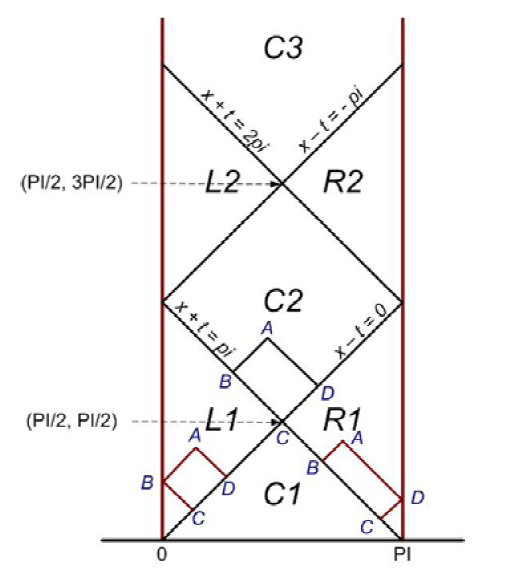
\includegraphics[width=0.7\textwidth]{Region.png}
 \end{figure}

\newpage
In region $C1$, the solution $u$ is defined by d\textsc{\char13}Alembert\textsc{\char13}s formula and the solution is

$$u(x,t)=\frac{1}{2}(0+0)+\frac{1}{2}\int_{x-t}^{x+t}1\cdot d\xi= t.$$

In region $L1$, let $A=(x,t)$ in $L1$ and thus $B=(0,t-x)$, $C=(\dfrac{t-x}{2}, \dfrac{t-x}{2})$, and $D=(\dfrac{x+t}{2}, \dfrac{x+t}{2})$. Using the parallelogram rule, we find that $u(x,t)=u(D_{C1})-u(C_{C1})=\dfrac{x+t}{2} - \dfrac{t-x}{2}=x$.

In region $R1$, let $A=(x,t)$ in $R1$ and thus $B=(\dfrac{\pi + x -t}{2},\dfrac{\pi - x +t}{2})$, $C=(\dfrac{3\pi -x -t}{2}, \dfrac{x+t - \pi}{2})$, and $D=(\pi, \dfrac{x+t-\pi}{2})$. Using the parallelogram rule, we find that $u(x,t)=u(B_{C1})-u(C_{C1}) =$ $\dfrac{\pi-x+t}{2} - \dfrac{x+t-\pi}{2}=\pi - x$.

In region $C2$, let $A=(x,t)$ in $C2$ and thus $B=(\dfrac{\pi + x -t}{2},\dfrac{\pi - x +t}{2})$, $C=(\dfrac{\pi}{2}, \dfrac{\pi}{2})$, and $D=(\dfrac{x+t}{2}, \dfrac{x+t}{2})$. Using the parallelogram rule, we find that $u(x,t)=u(B_{L1})+u(D_{R1})-u(C_{C1})=\dfrac{\pi + x -t}{2} + \pi - \dfrac{x+t}{2} -\dfrac{\pi}{2}=\pi - t$.

\phantomsection
\subsection{\textbf{3.1.3}} Consider the initial/boundary value problem:

\[
  \begin{cases}
  u_{tt}-u_{xx}=0,  &\text{for $0<x<\pi$ and $t>0$}, \\
  u(x,0)=x, u_t(x,0)=0, & \text{for $0<x<\pi$}, \\
  u_x(0,t)=0, u_x(\pi,t)=0, & \text{for $t\geq0$}.
  \end{cases}
\]

\begin{enumerate}[label=(\alph*)]
    \item Find a Fourier series solution, and sum the series in regions bounded by characteristics. Do you think that the solution is unique?
\end{enumerate}

We first want to find a Fourier series solution. We need to find $u(x,t)$ in the form

$$u(x,t)=\frac{a_0(t)}{2}+\sum_{n=1}^{\infty}a_n(t)\cos(nx)+\sum_{n=1}^{\infty}b_n(t)\sin(nx),$$

where $a_n(t)$ and $b_n(t)$ are determined by the boundary conditions. Hence,

$$u_x(x,t)=\sum_{n=1}^{\infty}-na_n(t)\sin(nx)+n b_n(t)\cos(nx),$$
$$u_x(x,0)=\sum_{n=1}^{\infty}n b_n(t)=0.$$

Therefore, $b_n(t)=0$ for every $n$. So, we can rewrite $u(x,t)$ as

$$u(x,t)=\frac{a_0(t)}{2}+\sum_{n=1}^{\infty}a_n(t)\cos(nx).$$

The partial differential equation is given as $u_{tt}-u_{xx}=0$. If we substitute $u(x,t)$ and solve through separation of variables we find that the functions $a_0(t)$ and $a_n(t)$ must satisfy the ordinary differential equations $a_0''(t)=0$ and $a_n''(t)+n^2a_n(t)=0$. The general solution to these equations are

$$a_0(t)=c_0(t)+d_0,$$
$$a_n(t)=c_n\sin(nt)+d_n\cos(nt).$$

If we differentiate both of these equations we will find that

$${a'_0}(t)=c_0,$$
$${a'_n}(t)=nc_n\cos(nt)-n d_n\sin(nt).$$

We can now use our remaining initial conditions to solve for $c_n$ and $d_n$. As $u(x,0)=x$ we have that

$$u(x,0)=\frac{a_0(0)}{2}+\sum_{n=1}^{\infty}a_n(0)\cos(nx)=\frac{d_0}{2}+\sum_{n=1}^{\infty}d_n\cos(nx)=x,$$

and as $u_t(x,0)=0$ we have that

$$u_t(x,t)=\frac{{a'_0}(t)}{2} + \sum_{n=1}^{\infty}{a'_n}(t)\cos(nx),$$
$$u_t(x,0)=\frac{{a'_0}(0)}{2} + \sum_{n=1}^{\infty}a'_n(0)\cos(nx)=\frac{c_0}{2}+\sum_{n=1}^{\infty}nc_n\cos(nx)=0.$$

Integrating and multiplying by $\cos(mx)$ produces

$$d_0=\pi,~~~ d_n=\frac{2}{\pi n^2}(\cos(n\pi) -1),~~~c_n=0. $$

Therefore, $a_0(t)=d_0=\pi$ and $a_n(t)=d_n\cos(nt)=\dfrac{2}{\pi n^2}(\cos(n\pi) -1)\cos(nt)$. Hence,

$$u(x,t)=\frac{a_0(t)}{2}+\sum_{n=1}^{\infty}a_n(t)\cos(nx)=\frac{\pi}{2}+\frac{2}{\pi}\sum_{k=1}^{\infty}\frac{(\cos(k\pi)-1)}{k^2}\cos(kt)\cos(kx).$$

\phantomsection
\subsection{\textbf{3.1.4}} Consider the initial boundary value problem:

\[
  \begin{cases}
  u_{tt}-c^2 u_{xx}=0,  &\text{for $x,t>0$}, \\
  u(x,0)=g(x), u_t(x,0)=h(x), & \text{for $x>0$}, \\
  u(0,t)=0,  & \text{for $t\geq0$},
  \end{cases}
\]

where $g(0)=0=h(0)$. If we extend $g$ and $h$ as odd functions on $-\infty<x<\infty$, show that d\textsc{\char13}Alembert\textsc{\char13}s formula (6) gives the solution.

We know that d\textsc{\char13}Alembert\textsc{\char13}s formula is

$$u(x,t)=\frac{1}{2}(g(x+ct)+g(x-ct)) + \frac{1}{2c}\int_{x-ct}^{x+ct}h(\xi)d\xi.$$

We are given that

$$u(x,0)=\frac{1}{2}(g(x)+g(x)) + \frac{1}{2c}\int_{x}^{x}h(\xi)d\xi=g(x).$$

We can calculate $u_t(x,t)$ by the FTC to form

$$u_t(x,t)=\frac{1}{2}(cg'(x+ct)-cg'(x-ct)) + \frac{1}{2c}(ch(x+ct)+ch(x-ct)),$$
$$u_t(x,0)=\frac{1}{2}(cg'(x)-cg'(x)) + \frac{1}{2c}(ch(x)+ch(x))=h(x),$$

where

$$u(0,t)=\frac{1}{2}(g(ct)+g(-ct))+\frac{1}{2c}\int_{-ct}^{ct}h(\xi)d\xi.$$

As $g(x)$ and $h(x)$ are odd functions we have that $g(-ct)=-g(ct)$. Hence,

$$u(0,t)=\frac{1}{2}(g(ct)+g(-ct))+\frac{1}{2c}\int_{-ct}^{ct}h(\xi)d\xi=0.$$

Where we can calculate further derivatives by

$$u_{tt}(x,t)=\frac{1}{2}(c^2g''(x+ct)+c^2g''(x-ct)) + \frac{1}{2}(ch'(x+ct)-ch'(x-ct)),$$
$$u_x(x,t)=\frac{1}{2}(g'(x+ct)+g'(x-ct)) + \frac{1}{2c}(h(x+ct)-h(x-ct)),$$
$$u_{xx}(x,t)=\frac{1}{2}(g''(x+ct)+g''(x-ct)) + \frac{1}{2c}(h'(x+ct)-h'(x-ct)).$$

Thus, $u_{tt}-c^2u_{xx}=0$ and d\textsc{\char13}Alembert\textsc{\char13}s formula (6) gives the solution.
\phantomsection
\subsection{\textbf{3.1.6}} Solve the initial/boundary value problem:

\[
  \begin{cases}
  u_{tt}-u_{xx}=1,  &\text{for $0<x<\pi$ and $t>0$}, \\
  u(x,0)=0, u_t(x,0)=0, & \text{for $0<x<\pi$}, \\
  u(0,t)=0, u(\pi,t)=-\pi^2/2, & \text{for $t\geq0$}.
  \end{cases}
\]

Describe the singularities (i.e., is $u$ $C^2$? If not, where does it fail? Is $u$ $C^1$? etc.)

We should first find a particular solution of the nonhomogeneous equation. This particular solution will reduce the problem to a boundary value problem for the homogeneous equation (as in 3.1.2 and 3.1.3).

Let\textsc{\char13}s find a particular solution. We will use a method similar to separation of variables. Assume that

$$u_p(x,t)=X(x).$$

Then, substituting into the PDE forms

$$-X''(x)=1 ~~~\implies~~~ X''(x)=-1.$$

We can integrate twice to find the solution of the PDE. The solution is

$$X(x)=-\frac{x^2}{2}+ax+b.$$

The boundary conditions form

$$u_p(0,t)=b=0,$$
$$u_p(\pi,t)=-\frac{(-\pi)^2}{2}+a\pi+b=\frac{-\pi^2}{2}~~~\implies~~~ a=0.$$

Hence, $a=b=0$ and the particular solution is

$$u_p(x,t)=-\frac{x^2}{2}.$$

The particular solution solves

\[
  \begin{cases}
  u_{p_{tt}}-u_{p_{xx}}=1,  &\text{for $0<x<\pi$ and $t>0$}, \\
  u_p(x,0)=-{x^2}/{2}, u_{p_t}(x,0)=0, & \text{for $0<x<\pi$}, \\
  u_p(0,t)=0, u_{p}(\pi,t)=-\pi^2/2, & \text{for $t\geq0$}.
  \end{cases}
\]

Next, we need to find a solution to the boundary value problem of the homogeneous equation

\[
  \begin{cases}
  u_{tt}-u_{xx}=0,  &\text{for $0<x<\pi$ and $t>0$}, \\
  u(x,0)={x^2}/{2}, u_t(x,0)=0, & \text{for $0<x<\pi$}, \\
  u(0,t)=0, u(\pi,t)=0, & \text{for $t\geq0$}.
  \end{cases}
\]

We can solve this through separation of variables. In fact, it is identical to 3.1.2 with $u(x,0)=1$ replaced by $u(x,0)={x^2}/{2}$.

Looking back to our solution of 3.1.2, we see that we need to change the initial condition for $c_n$ to

$$u_t(x,0)=\sum_{n=1}^{\infty}nc_n\sin(nx)=\frac{x^2}{2},$$

which produces

$$c_n=\frac{2}{n\pi}}\int_0^{\pi}\frac{x^2}{2}\sin(nx)dx=\frac{(2-\pi^2n^2)\cos(n\pi)+2n\pi\sin(n\pi)-2}{\pi n^4},&~~~~~~\text{for every n}.$$

Hence, we can solve the homogeneous equation $u_h(x,t)$. The solution is

\begin{align*}
\begin{split}
u_h(x,t)&=\sum_{n=1}^{\infty}c_n\sin(nt)\sin(nx) \\
&=\sum_{n=1}^{\infty}\frac{(2-\pi^2n^2)\cos(n\pi)+2n\pi\sin(n\pi)-2}{\pi n^4}\sin(nt)\sin(nx).
\end{split}
\end{align*}

We can then find $u(x,t)$. We have that $u(x,t)=u_h(x,t)+u_p(x,t)$ and therefore

$$u(x,t)=\sum_{n=1}^{\infty}\frac{(2-\pi^2n^2)\cos(n\pi)+2n\pi\sin(n\pi)-2}{\pi n^4}\sin(nt)\sin(nx)-\frac{x^2}{2}.$$

\phantomsection
\subsection{\textbf{3.2.2}} Find the solution of the initial value problem

\[
  \begin{cases}
  u_{tt}=u_{xx} + u_{yy} + u_{zz}, \\
  u(x,y,z,0)=x^2+y^2, ~u_t(x,y,z,0)=0,
  \end{cases}
\]

(a) by using (37) and (b) by using (39).

First, we will apply Kirchoff\textsc{\char13}s formula to find the solution. Letting $(\xi,\eta,\zeta)$ denote a point on the unit sphere $S^2\subset\mathbb R^3$ and $dS$ be the surface area element on $S^2$, we see that (as $h(x)=0)$)

\begin{align*}
\begin{split}
u(x,y,z,t)&=\frac{\partial}{\partial t}\Bigg(\frac{t}{4\pi}\int_{S^2}\Big[(x+t\xi)^2+(y+t\eta)^2\Big]dS\Bigg) \\ &=
\frac{\partial}{\partial t}\Bigg(\frac{t}{4\pi}\int_{S^2}\Big[x^2+2xt\xi+t^2\xi^2+y^2+2yt\eta+t^2\eta^2]dS\Bigg) \\ &=
\frac{\partial}{\partial t}\Bigg(\frac{t}{4\pi}\Big[4\pi(x^2+y^2)+2xt\int_{S^2}\xi dS + 2yt \int_{S^2}\eta dS + t^2\int_{S^2}\xi^2 dS +  t^2\int_{S^2}\eta^2 dS\Big]\Bigg).
\end{split}    
\end{align*}

Although,

$$\int_{S^2}\xi dS=0,$$

which can be verified through explicit calculation using spherical coordinates, or by symmetry (just split $S^2$ into the hemispheres $\xi\geq 0$ and $\xi\leq 0$. You will find that the two integrals cancel out). By the same reasoning, $\int_{S^2}\eta dS=0$. Therefore, by the rotational symmetry of the sphere we have that

$$\int_{S^2}\xi^2 dS=\int_{S^2}\eta^2 dS=\int_{S^2}\zeta^2 dS \implies \int_{S^2}\xi^2 dS=\frac{1}{3}\int_{S^2}(\xi^2+\eta^2+\zeta^2)dS=\frac{1}{3}\int_{S^2}dS=\frac{4\pi}{3}.$$

Hence, we can conclude that

$$u(x,y,z,t)=\frac{\partial}{\partial t}\Bigg(\frac{t}{4\pi}\Big[4\pi(x^2+y^2)+t^2\frac{8\pi}{3}\Big]\Bigg)=x^2+y^2+2t^2.$$

For (b), we need to use the 2d formula given in (39). This is possible since the data are independent of $z$. Let\textsc{\char13}s denote $(\xi,\eta)$ as a point on the unit disk $D = \{(\xi,\eta) : \xi^2 + \eta^2 < 1\}$ in the plane. Then (once again, $h(x)=0)$,

\begin{align*}
\begin{split}
u(x,y,z,t)&=\frac{\partial}{\partial t}\Bigg(\frac{t}{2\pi}\int_{D}\frac{(x+t\xi)^2+(y+t\eta)^2}{\sqrt{1-\xi^2-\eta^2}}d\xi d\eta\Bigg) \\ &=
\frac{\partial}{\partial t}\Bigg(\frac{t}{2\pi}\int_{D}\frac{x^2+y^2+2xt\xi+2yt\eta+t^2(\xi^2+\eta^2) }{\sqrt{1-\xi^2-\eta^2}}d\xi d\eta\Bigg) \\ &=
\frac{\partial}{\partial t}\Bigg(\frac{t}{2\pi}\Bigg[(x^2+y^2)\int_{D}\frac{d\xi d\eta}{\sqrt{1-\xi^2-\eta^2}}+2xt\int_{D}\frac{\xi d\xi d\eta}{\sqrt{1-\xi^2-\eta^2}}\\ 
&~~~~~~~~~+2yt\int_{D}\frac{\eta d\xi d\eta}{\sqrt{1-\xi^2-\eta^2}}+t^2\int_{D}\frac{(\xi^2+\eta^2) d\xi d\eta}{\sqrt{1-\xi^2-\eta^2}}\Bigg]\Bigg).
\end{split}    
\end{align*}

So, by symmetry

$$\int_{D}\frac{\xi d\xi d\eta}{\sqrt{1-\xi^2-\eta^2}}=\int_{D}\frac{\eta d\xi d\eta}{\sqrt{1-\xi^2-\eta^2}}=0.$$

Thus, if we switch to polar coordinates $(r,\theta)$ in the plane, we see that

$$\int_{D}\frac{d\xi d\eta}{\sqrt{1-\xi^2-\eta^2}}=\int_0^1\int_0^{2\pi}\frac{rdrd\theta}{\sqrt{1-r^2}}=2\pi\int_0^1\frac{rdr}{\sqrt{1-r^2}}=\pi\int_0^1\frac{ds}{\sqrt{s}}=2\pi,$$

and

$$\int_{D}\frac{(\xi^2+\eta^2) d\xi d\eta}{\sqrt{1-\xi^2-\eta^2}}=\int_0^1\int_0^{2\pi}\frac{r^2(rdrd\theta)}{\sqrt{1-r^2}}=2\pi\int_0^1\frac{r^3dr}{\sqrt{1-r^2}}=\pi\int_0^1\frac{(1-s)ds}{\sqrt{s}}=\frac{4\pi}{3}.$$

Hence, we can conclude that

$$u(x,y,z,t)=\frac{\partial}{\partial t}\Bigg(\frac{t}{2\pi}\Big[2\pi(x^2+y^2)+t^2\frac{4\pi}{3}\Big]\Bigg)=x^2+y^2+2t^2.$$

\phantomsection
\subsection{\textbf{3.2.3}} Use Duhamel\textsc{\char13}s principle to find the solution of the nonhomogenuous wave equation for three space dimensions $u_{tt}-c^2\Delta u=f(x,t)$ with initial conditions $u(x,0)=0=u_t(x,0)$. What regularity in $f(x,t)$ is required for the solution $u$ to be $C^2$.

We are given the nonhomogeneous wave equation with the following initial conditions

\[
  \begin{cases}
  u_{tt}-c^2\Delta u=f(x,t), \\
  u(x,0)=0=u_t(x,0).
  \end{cases}
\]

By Duhamel\textsc{\char13}s principle, we reduce the problem to the special homogeneous equations with
nonhomogeneous initial conditions

\[
  \begin{cases}
  U_{tt}-c^2\Delta U=0, &\text{for $x\in\mathbb R$, $t>0$, $s\geq 0$},\\
  U(x,0,s)=0, &\text{for $x\in\mathbb R$, $s\geq 0$},\\
  U_t(x,0,s)=f(x,s), &\text{for $x\in\mathbb R$, $s\geq 0$}.
  \end{cases}
\]

Then, we have that

$$u(x,t)=\int_0^t U(x,t-s,s)ds,$$

solves the nonhomogeneous wave equation. With three spacial dimensions we can apply Kirchhoff\textsc{\char13}s formula (with $g(x)=0$ and $h(x)=f(x)$) to see that

$$U(x,t,s)=\frac{1}{4\pi}\frac{\partial}{\partial t}\Bigg(t\int_{|\xi|=1} 0 dS_{\xi}\Bigg) + \frac{t}{4\pi}\int_{|\xi|=1} f(x+ct\xi,s)dS_{\xi}=\frac{t}{4\pi}\int_{|\xi|=1} f(x+ct\xi,s)dS_{\xi}.$$

Therefore,

\begin{align*}
\begin{split}
u(x,t)=\int_0^t U(x,t-s,s)ds &= \int_0^t \Bigg(\frac{t-s}{4\pi}\int_{|\xi|=1} f(x+c(t-s)\xi,s)dS_{\xi} \Bigg)ds \\ &= \frac{1}{4\pi}\int_0^t\int_{|\xi|=1} (t-s)f(x+c(t-s)\xi,s)dS_{\xi} ds.
\end{split}
\end{align*}

Hence, we see that $f(x,t)$ needs to be $C^2$ in $x$ and $C^0$ in $t$ for the solution $u$ to be $C^2$.


\phantomsection
\subsection{\textbf{3.2.4}} Let $\Omega=\{(x,y)\in\mathbb R^2 : \text{$0<x<a$ and $0<y<b$}\}$, and use separation of variables to solve the initial/boundary value problem

\[
  \begin{cases}
    u_{tt}=u_{xx}+u_{yy}, & \text{for $(x,y)\in\Omega$ and $t>0$}, \\
    u(x,y,t)=0, & \text{for $(x,y)\in\partial\Omega$ and $t>0$}, \\
    u(x,y,0)=\sin{\dfrac{\pi x}{a}}\sin{\dfrac{2\pi y}{b}}, ~\text{and}~u_t(x,y,0)=0, & \text{for $(x,y)\in\Omega$}.
  \end{cases}
\]

Letting $u(x,y,t)=X(x)Y(y)T(t)$, we form

$$XYT''=X''YT + XY''T.$$

If we divide every term by $XYT$, we get

$$\frac{T''}{T} = \frac{X''}{X} + \frac{Y''}{Y},$$

which must be equal to some constant $\lambda$. Therefore,

$$\frac{T''}{T} = \frac{X''}{X} + \frac{Y''}{Y} = - \lambda. $$

Then, acknowledging that $\frac{X''}{X}=-\mu^2, \frac{Y''}{Y}=-\nu^2$, and $\frac{T''}{T}=-\omega^2$ are constants, we see that

$$\lambda=\mu^2+\nu^2 + \omega^2.$$

Our initial condition tells us that

$$u(x,y,0)=\sin{\dfrac{\pi x}{a}}\sin{\dfrac{2\pi y}{b}}.$$

So, we know that

$$u(x,y,0)=X(x)Y(y)T(0)=\sin{\dfrac{\pi x}{a}}\sin{\dfrac{2\pi y}{b}}.$$

Hence, we need to find $T(t)$. Our initial conditions are

\[
  \begin{cases}
  T''+\omega^2 T=0, \\
  T(0)=\sin{\dfrac{\pi x}{a}}\sin{\dfrac{2\pi y}{b}},~~ T'(0)=0.
  \end{cases}
\]

Using these alongside the initial condition, $u(x,y,t)=0$, we find that

$$T(t)=\cos\bigg(\frac{\pi(4a^2+b^2)^{\frac{1}{2}}t}{ab}\bigg).$$

Therefore, our solution is

$$u(x,y,z)=X(x)Y(y)T(t)=sin{\dfrac{\pi x}{a}}\sin{\dfrac{2\pi y}{b}}\cos\bigg(\frac{\pi(4a^2+b^2)^{\frac{1}{2}}t}{ab}\bigg).$$

\phantomsection
\subsection{\textbf{3.2.5}} Find a formula for the solution $v(x,t)=v(x_1,x_2,t)$ of the Cauchy problem for the two-dimensional Klein-Gordon equation:

\[
  \begin{cases}
  v_{tt}=c^2\Delta v - m^2v, ~~~ \text{for $x\in\mathbb R^2$ and $t>0$}, \\
  v(x,0)=g(x),~~~~~~v_t(x,0)=h(x).
  \end{cases}
\]

Using the hint in the back of the book, we define

$$u(x,y,z,t)=\cos\left(\frac{m}{c}z\right)v(x,y,t).$$

Where we can perform a calculation to see that $u$ satisfies the wave equation in 3d, so it is represented by Kirchhoff\textsc{\char13}s formula. Let's assume that $g=0$. Then, letting $(\xi,\eta,\zeta)$ denote a point on the unit sphere $S^2\subset\mathbb R^3$, we see that

$$u(x,y,z,t)=\frac{t}{4\pi}\int_{S^2}\cos\Big(\frac{m}{c}(z+ct\zeta)\Big)h(x+ct\xi,y+ct\eta)dS(\xi,\eta,\zeta).$$

If we let $z=0$, then

$$v(x,y,t)=u(x,y,0,t)=\frac{t}{4\pi}\int_{S^2}\cos(mt\zeta)h(x+ct\xi,y+ct\eta)dS(\xi,\eta,\zeta).$$

So, we now follow the derivation of the solution formula for the wave equation in 2d. We will parametrize the hemispheres $\zeta \geq 0$ and $\zeta \leq 0$ of $S^2$ as graphs

$$\zeta = \pm\sqrt{1-\xi^2-\eta^2},$$

over the unit disk $D = \{(\xi,\eta) : \xi^2 + \eta^2 \leq 1\}$. This will transform the integral to (observing that the cosine function is even, so there is no difference between the integrals in the two hemispheres)

$$v(x,y,t)=\frac{t}{2\pi}\int_D \frac{\cos\Big(mt\sqrt{1-\xi^2-\eta^2}\Big)h(x+ct\xi,y+ct\eta)}{\sqrt{1-\xi^2-\eta^2}}d\xi d\eta.$$

If we now remove the restriction that $g=0$, we can calculate the general form as
\begin{align*}
\begin{split}
v(x,y,t)=\frac{\partial}{\partial t}\Bigg(\frac{t}{2\pi}\int_D\frac{\cos\Big(mt\sqrt{1-\xi^2-\eta^2}\Big)g(x+ct\xi,y+ct\eta)}{\sqrt{1-\xi^2-\eta^2}}d\xi d\eta\Bigg) +\\ \frac{t}{2\pi}\int_D \frac{\cos\Big(mt\sqrt{1-\xi^2-\eta^2}\Big)h(x+ct\xi,y+ct\eta)}{\sqrt{1-\xi^2-\eta^2}}d\xi d\eta.
\end{split}
\end{align*}


\phantomsection
\subsection{\textbf{3.3.1}} Let $\Omega$ be a smooth, bounded domain in $\mathbb R^n$. For a $C^2$ solution $u(x,t)$ of the wave equation $u_{tt}=c^2\Delta u$ for $x\in\Omega,t>0$, define the energy to be $\textepsilon_{\Omega}(t)=\frac{1}{2}\int_{\Omega}(u_t^2+c^2|\nabla u|^2)$ dx. If $u$ satisfies either the boundary condition $u(x,t)=0$ or $\partial u / \partial \nu(x,t)=0$ for $x\in\partial\Omega$, where $\nu$ is the exterior unit normal, then show that $\textepsilon_{\Omega}(t)$ is constant.

We consider solutions to the wave equation

$$u_{tt}=c^2\Delta u, ~~~~~u=u(x,t),  ~~~~~x\in\Omega,t>0,$$

which have a Dirichlet boundary condition

$$u(x,t)=0, ~~~~~\text{for all $x\in\partial\Omega,t\geq 0$},$$

or a Neumann boundary condition

$$\nabla u \cdot \nu = \frac{\partial u}{\partial \nu}(x,t)=0,~~~~~\text{for all $x\in\partial\Omega,t\geq 0$}.$$

We should assume that $u$ belongs to the space

$$u\in C^2(\overline{\Omega}\times(0,\infty))\cap C^1(\overline{\Omega}\times[0,\infty)).$$

We need to show that energy 

$$\textepsilon_{\Omega}(t)=\frac{1}{2}\int_{\Omega}(u_t^2+c^2|\nabla u|^2) ~dx,$$

is conserved. If we take the first derivative with respect to $t$, we find that

$$\frac{d}{dt}\textepsilon_{\Omega}(t)=\frac{d}{dt}\Bigg(\frac{1}{2}\int_{\Omega}(u_t^2+c^2|\nabla u|^2) ~dx\Bigg) =\int_{\Omega}(u_tu_{tt}+c^2\nabla u \cdot \nabla u_t)~ dx.$$

But, we know from Green's first identity that

$$\int_{\partial\Omega}v\frac{\partial u}{\partial \nu}dS = \int_{\Omega}(v \Delta u + \nabla v \cdot \nabla u)~dx.$$

Letting $v=u_t$, we see that

$$\int_{\Omega}\nabla u \cdot \nabla u_t ~dx = \int_{\partial\Omega}u_t\frac{\partial u}{\partial \nu}dS - \int_{\Omega}u_t\Delta u~ dx,$$

and the middle term vanishes because of the Dirichlet or Neumann boundary conditions. For the Neumann boundary condition, we have that $\frac{\partial u}{\partial \nu}=0$ on $\partial\Omega$. For the Dirichlet boundary condition, we have that $u=0$ on $\partial\Omega ~\implies$ $u_t=0$ on $\partial\Omega$. Hence, 

$$\int_{\Omega}\nabla u \cdot \nabla u_t ~dx =  - \int_{\Omega}u_t\Delta u~ dx,$$

and therefore

$$\frac{d}{dt}\textepsilon_{\Omega}(t)=\int_{\Omega}(u_tu_{tt}-c^2u_t\Delta u) ~dx= \int_{\Omega}u_t(u_{tt}-c^2\Delta u)~ dx=0.$$

Thus, energy is conserved.

\phantomsection
\subsection{\textbf{3.3.2}} Use the previous exercise to show uniqueness of the solution for the (nonhomogenuous) wave equation $u_{tt}=\Delta u + f(x,t)$ in a smooth, bounded domain $\Omega\subset\mathbb R^n$ with either (a) Dirichlet condition $u=g$ on $\partial\Omega$, or (b) Neumann condition $\partial u/\partial \nu=h$ on $\partial\Omega$.

We need to prove uniqueness of solutions to the initial boundary value problem

\[
  \begin{cases}
  u_{tt}-c^2\Delta u=f(x,t), &\text{for $x\in\Omega$, $t>0$,} \\
  u(x,t)=\gamma(x,t), &\text{for $x\in\partial\Omega$, $t>0$}, \\
  u(x,0)=g(x), u_t(x,0)=h(x),& \text{for $x\in\Omega$}, 
  \end{cases}
\]

where $f ,\gamma, g ,h$ are given functions, and $u$ is assumed to belong to the space

$$u\in C^2(\Omega\times(0,\infty))\cap C^1(\overline{\Omega}\times[0,\infty)).$$

Let\textsc{\char13}s assume that $u,v$ both belong this space and solve the initial boundary value problem defined above. Then, $w=u-v$ also solves the initial boundary value problem with $f=0,$ $\gamma=0,$ $g=0$, and $h=0$. So, by the previous exercise, we see that the energy in $\Omega$ must be zero for all $t\geq 0$ as all of the functions are zero. Hence,

$$\textepsilon_{\Omega}(t)=\textepsilon_{\Omega}(0)=0.$$

Although, as $\textepsilon_{\Omega}(t)$ is defined by $\textepsilon_{\Omega}(t)=\frac{1}{2}\int_{\Omega}(w_t^2+c^2|\nabla w|^2)$ dx=0, it must be that $w_t=0$ and $\nabla w=0$ in $\Omega\times[0,\infty)$. Therefore, $w=\hspace{1mm}$constant and this constant must be zero as $w=0$ at time $t=0$. So, $w=0 ~\implies~ u=v$.

An analogous argument holds if we replace the Dirichlect boundary condition with the Neumann boundary condition.

\phantomsection
\subsection{\textbf{3.3.4}} The partial differential equation $u_{tt}=c^2\Delta u -q(x)u$ arises in the study of wave propogation in a nonhomogenuous elastic medium: $q(x)$ is nonnegative and proportional to the coefficient of elasticity at $x$.

\begin{enumerate}[label=(\alph*)]
    \item Define an appropriate notion of energy for solutions.
    \item Verify the corresponding energy inequality.
    \item Use the energy method to prove that solutions are uniquely determined by their Cauchy data.
\end{enumerate}

(a) The energy integral is

$$\textepsilon(t)=\frac{1}{2}\int_{\Omega}(|u_t|^2+c^2|\nabla u|^2+q(x)u^2) dx.$$

We can verify this by differentiating with respect to $t$ to obtain

$$\frac{d}{dt}\textepsilon(t)=\frac{1}{2}\int_{\Omega}(u_tu_{tt}+c^2\sum_{i=1}^n u_{x_i}u_{x_i}t + q(x)uu_t) dx.$$

Integrating by parts then produces

$$\frac{d}{dt}\textepsilon(t)=\int_{\Omega}u_t\big(u_{tt}-c^2\Delta u +q(x)\big)dx=0,$$

which shows that $\textepsilon(t)$ must be a constant.

(b) For any time $\uptau\in[0,t_0]$, let $\overline{B}_{\uptau}=\{x\in\mathbb R^n:|x-x_0|\leq c(t_0-\uptau)\}$. Consider the local energy function

\begin{equation}
E_{x_0,t_0}(\uptau)=\frac{1}{2}\int_{B_{\uptau}}(u_t^2+c^2|\nabla u|^2+q(x)u^2)\big|_{t=\uptau}dx, ~~~~~~~\text{for $0\leq \uptau\leq t_0$}.
\end{equation}

We claim that (1) is a nonincreasing function of $\uptau$; that is, the following energy inequality holds:

\begin{equation}
E_{x_0,t_0}(\uptau)\leq E_{x_0,t_0}(0), ~~~~~~~\text{for $0\leq \uptau\leq t_0$}.
\end{equation}

To prove (2), we introduce the following notations

$$\Omega_{\uptau}=\{(x,t):|x-x_0|< c(t_0-t),0<t<\uptau\},$$
$$C_{\uptau}=\{(x,t):|x-x_0|= c(t_0-t),0<t<\uptau\}.$$

Notice that $\partial\Omega_{\uptau}=C_{\uptau}\cup(\overline{B}_0\times\{0\})\cup(\overline{B}_{\uptau}\times\{\uptau\})$, where the unions are disjoint. Moreover, the exterior unit normal $\nu$ on $\partial\Omega_{\uptau}$ is given on $\overline{B}_{\uptau}\times\{\uptau\}$ by $\nu=\langle 0,\dots,0,1 \rangle$, and on $\overline{B}_0$ by $\nu=\langle 0,\dots,0,-1 \rangle$. On $C_{\uptau}$, the normal $\nu=\langle \nu_1,\dots,\nu_n,\nu_{n+1} \rangle$ satisfies $c^2(\nu_1^2 + \cdots + \nu_n^2)=\nu_{n+1}^2$; together with the unit length condition $\nu_1^2 + \cdots + \nu_n^2 + \nu_{n+1}^2=1$, this implies

$$\nu_1^2 + \cdots + \nu_n^2=\frac{\nu_{n+1}^2}{c^2}=\frac{1}{1+c^2}.$$

Given a solution $u$, we define the vector field

$$\vec{V}=\langle 2c^2u_tu_{x_1},\dots,2c^2u_tu_{x_n},-(c^2|\nabla u|^2+u_t^2+q(x)u^2)\rangle.$$

If we calculate the divergence in $(x,t)$, we find

\begin{align*}
\begin{split}
\text{div} ~\vec{V}=2c^2(u_{tx_1}u_{x_1}+u_tu_{x_1x_1}+\cdots+u_{tx_n}u_{x_n}+u_tu_{x_nx_n})\\~-
        2c^2(u_{tx_1}u_{x_1}+\cdots+u_{tx_n}u_{x_n})-2u_tu_{tt}-2q(x)uu_t=0.
\end{split}
\end{align*}

The divergence theorem therefore implies

$$\int_{\partial\Omega_{\uptau}}\vec{V}\cdot\nu dS=0.$$

Now, on $C_{\uptau}$, the following inequality holds

$$2u_t(u_{x_1}\nu_1+\cdots+u_{x_n}\nu_n)\leq \frac{c}{\sqrt{1+c^2}}|\nabla u|^2 + \frac{1}{c\sqrt{1+c^2}}(u_t^2+q(x)u^2).$$

Therefore, we may compute on $C_{\uptau}$

$$\vec{V}\cdot\nu=2c^2u_t(u_{x_1}\nu_1+\cdots+u_{x_n}\nu_n)-(c^2|\nabla u|^2+{u_t}^2+q(x)u^2)\nu_{n+1}\leq 0,$$

so in particular

$$\int_{C_{\uptau}}\vec{V}\cdot\nu dS \leq 0.$$

Then, we have

\begin{align*}
\begin{split}
0 &\leq \int_{\overline{B}_0} \vec{V}\cdot\nu dS + \int_{\overline{B}_{\uptau}\times\{\uptau\}} \vec{V}\cdot\nu dS \\&=
\int_{\overline{B}_0}(c^2|\nabla u|^2+{u_t}^2+q(x)u^2)\big|_{t=0} dx - \int_{\overline{B}_{\uptau}} (c^2|\nabla u|^2+{u_t}^2+q(x)u^2)\big|_{t=\uptau} dx,
\end{split}
\end{align*}

which proves (2),

\begin{equation*}
E_{x_0,t_0}(\uptau)\leq E_{x_0,t_0}(0), ~~~~~~~\text{for $0\leq \uptau\leq t_0$}.
\end{equation*}

(c) Let both $u$ and $v$ be solutions to $u_{tt}=c^2\Delta u - q(x)u$ on $C^2(\Omega\times(0,\infty))$ with initial conditions $u(x,0)=g(x), u_t(x,0)=h(x)$ for $x\in\Omega$. Let $w\equiv u -v$, then

\[
  \begin{cases}
  w_{tt}=c^2\Delta w - q(x)w, &\text{for $x\in\Omega$, $t>0$}, \\
  w(x,0)=w_t(x,0)=0, &\text{for $x\in\Omega$} .
  \end{cases}
\]

Hence, we know that $\textepsilon(t)=\textepsilon(0)=0$. It follows that

$$\textepsilon(t)=\frac{1}{2}\int_{\Omega}(|w_t|^2+c^2|\nabla w|^2+q(x)w^2) dx=0,$$

since $q(x)$ is nonnegative and the third term implies that $w(x,t)\equiv 0$. Therefore, $u(x,t)\equiv v(x,t)$.

\phantomsection
\section{Chapter 4 Solutions}

\phantomsection
\subsection{\textbf{4.1.1}} Let $\Omega=\{(x,y)\in\mathbb R^2 : x^2+y^2<1\}=\{(r,\theta):0\leq r <1, 0 \leq \theta < 2\pi\}$, and use separation of the variables $(r,\theta)$ to solve the Dirichlet problem

\[
  \begin{cases}
  \Delta u = 0, & \text{in $\Omega$}, \\
  u(1,\theta) =g(\theta), & \text{for $0\leq \theta < 2\pi$}.
  \end{cases}
\]

It is natural to use polar coordinates $(r,\theta)$ in which the problem becomes

\[
  \begin{cases}
  \dfrac{\partial^2 u}{\partial r^2} + \dfrac{1}{r}\dfrac{\partial u}{\partial r} + \dfrac{1}{r^2}\dfrac{\partial^2 u}{\partial \theta^2}=0, & \text{for $0\leq r < 1$, $0\leq \theta < 2\pi$}, \\
  u(1,\theta) =g(\theta), & \text{for $0\leq \theta < 2\pi$}.
  \end{cases}
\]

If we write $r=e^{-t}$ ad $u(r,\theta)=X(t)Y(\theta)$, then

$$r^2\partial_r^2 u + r\partial_r u + \partial_{\theta}^2 u = \partial_t^2 u + \partial_{\theta}^2 u = X''(t)Y(\theta)+X(t)Y''(\theta)=0.$$

Separating the variables, we obtain

$$\frac{X''(t)}{X(t)}=-\frac{Y''(\theta)}{Y(\theta)}=\lambda.$$

But $Y''(\theta)+\lambda Y(\theta)=0$ has solutions $\lambda_n=n^2$ and $Y_n(\theta)=a_n\cos n\theta $ $+ b_n\sin n\theta$; notice $Y_0(\theta)=a_0=$const. The equation $X''(t)+n^2X(t)=0$ has solutions $X_0(t)=c_0 t + d_0$ and $X_n(t)=c_n e^{nt}+ d_n e^{-nt}$ for $n=1,2,3,\dots$ . This means that $u_0(r,\theta)=-c_0\log r + d_0$ and $u_n(r,\theta)=(a_n \cos n\theta + b_n\sin n\theta)$ $(c_n r^{-n} + d_n r^n)$ for $n=1,2,3,\dots$ . But $u$ must be finite at $r=0$, so $c_n=0$. By superposition we may write (after relabeling coefficients)

$$u(r,\theta)=a_0+\sum_{n=1}^{\infty}r^n(a_n \cos n\theta + b_n\sin n\theta).$$

But then

$$u(1,\theta)=a_0+\sum_{n=1}^{\infty}(a_n \cos n\theta + b_n\sin n\theta)=g(\theta),$$

which shows that the coefficients $a_n$,$b_n$ for $n\geq 1$ are determined from the Fourier series for $g(\theta)$. Therefore,

$$a_n=\frac{1}{\pi}\int_0^{2\pi}g(\theta)\cos(n\theta)d\theta &~~~~~ \text{for $n=1,2,3\dots$},$$
$$b_n=\frac{1}{\pi}\int_0^{2\pi}g(\theta)\sin(n\theta)d\theta&~~~~~ \text{for $n=1,2,3\dots$}.$$
Notice, however that $a_0$ is not determined by $g(\theta)$ and therefore may take any arbitrary value. Moreover, the constant term in the Fourier series for $g(\theta)$ must be zero. So, we can write

$$a_0=\frac{1}{2\pi}\int_0^{2\pi}g(\theta)d\theta.$$

\phantomsection
\subsection{\textbf{4.1.2}} Let $\Omega=(0,\pi)\times(0,\pi)$, and use separation of variables to solve the mixed boundary value problem

\[
  \begin{cases}
  \Delta u = 0, & \text{in $\Omega$}, \\
  u_x(0,y)=0=u_x(\pi,y), & \text{for $0 < y < \pi$}, \\
  u(x,0)=0,~~ u(x,\pi)=g(x), & \text{for $0 < x < \pi$}.
  \end{cases}
\]

Assume $u(x,y)=X(x)Y(y)$. Substitution into the PDE produces

$$X''(x)Y(y)+X(x)Y''(y)=0.$$

Separating the variables, we obtain

$$\frac{X''(x)}{X(x)}=-\frac{Y''(y)}{Y(y)}=-\lambda.$$

For the first equation, consider $X''(x)+\lambda X(x)=0$. If $\lambda = 0$, then $X''(x)=0$ and we can simplify this to find $X_0(x)=a_0x + b_0$.

Else, if $\lambda \neq 0$ then we need to solve $X''(x)+\lambda X(x)=0$. By standard ODE techniques, we find that the roots of the characteristic polynomial are $r=\pm i\lambda$. Therefore, we see that $X_n(x)=a_n\cos nx + b_n\sin nx$.

The boundary conditions are $u_x(0,y)=0=u_x(\pi,y)$. So,

$$u_x(0,y)=X'(0)Y(y)=0 ~~~\implies~~X'(0)=0,$$
$$u_x(\pi,y)=X'(\pi)Y(y)=0 ~~~\implies~~X'(\pi)=0.$$

Hence, $X_0'(0)=a_0=0$ and $X_n'(0)=n b_n = 0 ~\implies~b_n=0$. Thus, $X_0(x)=b_0$ and $X_n(x)=a_n\cos nx$.

If we return back to our original equation $X''(x)+\lambda X(x)=0$, we can substitute in the above form to find that $-n^2 a_n \cos nx + \lambda a_n \cos nx = 0$. This implies that

$$\lambda = n^2 ~~~~~ &\text{for $n=1,2,3,\dots$ .}$$

So, we now consider $Y''(y)-\lambda Y(y)=0$ or $Y''(y)-n^2 Y(y)=0$. If $n=0$, then we have $Y''(y)=0$ and we can simplify this to find $Y_0(y)=c_0 y + d_0$.

Else, if $n \neq 0$ then we need to solve $Y''(y)-n^2 Y(y)=0$. By standard ODE techniques, we find that the roots of the characteristic polynomial are $r=\pm n$. Therefore, we see that $Y_n(y)=c_n e^{ny} + d_n e^{-ny}$.

The boundary condition is $u(x,0)=0$. So,

$$u(x,0)=0=X(x)Y(0)=0 ~~~\implies~~Y(0)=0.$$

Hence, $Y_0(0)=d_0=0$ and $Y_n(0)=c_n + d_n=0  ~\implies~c_n=-d_n$. Thus, $Y_0(y)=c_0y$ and $Y_n(y)=c_n(e^{ny}-e^{-ny})=\widetilde{c_n}\sinh ny$.

If we put everything together, we form

$$u_0(x,y)=X_0(x)Y_0(y)=b_0c_0 y = \widetilde{a_0} y,$$
$$u_n(x,y)=X_n(x)Y_n(y)=(a_n\cos nx)(\widetilde{c_n}\sinh ny) = \widetilde{a_n} \cos nx \sinh ny.$$

So, by superposition, we can write

$$u(x,y)=\widetilde{a_0} y + \sum_{n=1}^{\infty}\widetilde{a_n} \cos nx \sinh ny.$$

The above equation satisfies the three homogeneous boundary conditions. For the non-homogeneous boundary condition, we have that $u(x,\pi)=g(x)$. So,

$$u(x,\pi)=\widetilde{a_0} \pi + \sum_{n=1}^{\infty}\widetilde{a_n} \cos nx \sinh n\pi=g(x).$$

By the orthogonality conditions of coefficients, we have that

$$\int_0^{\pi}g(x)dx= \int_0^{\pi}(\widetilde{a_0} \pi + \sum_{n=1}^{\infty}\widetilde{a_n} \cos nx \sinh n\pi)dx = \widetilde{a_0} \pi^2 ~~\implies~~\widetilde{a_0}=\frac{1}{\pi^2}\int_0^{\pi}g(x)dx,$$

$$\int_0^{\pi}g(x)\cos mx ~dx= \sum_{n=1}^{\infty}\widetilde{a_n}\sinh  n\pi \int_0^{\pi}\cos nx \cos mx~dx=\frac{\pi}{2}\widetilde{a_m}\sinh m\pi,$$

which implies that

$$\widetilde{a_n}\sinh n\pi=\frac{2}{\pi}\int_0^{\pi}g(x)\cos nx ~dx.$$


\phantomsection
\subsection{\textbf{4.1.3}} Prove that the solution of the Robin or third boundary value problem (5) for the Laplace equation is unique when $\alpha>0$ is a constant.

We have that

\[
  \begin{cases}
  \Delta u = 0, & \text{in $\Omega$}, \\
  \frac{\partial u}{\partial \nu} + \alpha u =\beta, & \text{on $\partial \Omega$},
  \end{cases}
\]

where $\alpha, \beta$ are constants with $\alpha > 0$. We need to prove uniqueness. Assume that

$$u,v \in C^2(\Omega)\cap C^1(\overline{\Omega}),$$

are both solutions to the Laplace equation. Let $w=u-v$. Then, w satisfies

\[
  \begin{cases}
  \Delta w = 0, & \text{in $\Omega$}, \\
  \frac{\partial w}{\partial \nu} + \alpha w =0, & \text{on $\partial \Omega$}.
  \end{cases}
\]

If we apply Green's first identity with $u,v=w$, we find that 

$$\int_{\partial\Omega} w \frac{\partial w}{\partial \nu}dS=\int_{\Omega}\nabla w \cdot \nabla w~dx=\int_{\Omega}|\nabla w|^2 dx.$$

If we now insert the boundary conditions, $\dfrac{\partial w}{\partial \nu} = -\alpha w$ on $\partial\Omega$, we find that

$$-a\int_{\partial\Omega} w^2 dS=\int_{\Omega}|\nabla w|^2 dx.$$

Therefore, in the formula above the LHS is always $\leq 0$ while the RHS is always $\geq 0$. So, both sides must equal zero. Hence, $w=0$ in $\Omega$. As we assumed that $w$ is continuous on the boundary, we also have that $w=0$ in $\overline{\Omega}$. Thus, u=v.

\phantomsection
\subsection{\textbf{4.1.4}} Let $\Omega$ be the unit disk as in Exercise 1.
\begin{enumerate}[label=(\alph*)]
    \item Solve the Robin problem (5) for the Laplace equation when $\alpha > 0$ is constant.
\end{enumerate}

We are given that the solution by separation of variables on the unit disk is

$$u(r,\theta)=a_0+\sum_{n=1}^{\infty}r^n(a_n \cos n\theta + b_n\sin n\theta),$$

where the normal derivative on the boundary can be represented as

$$u_r(1,\theta)=\sum_{n=1}^{\infty}n(a_n \cos n\theta + b_n\sin n\theta).$$

So, we need to consider the new boundary condition of 

$$\frac{\partial u}{\partial \nu} + \alpha u =\beta, & ~~~~~\text{on $\partial \Omega$}.$$

Through this new boundary condition, we can write the equation above as

$$\beta(\theta)=\alpha a_0+\sum_{n=1}^{\infty}(\alpha+ n)(a_n \cos n\theta + b_n\sin n\theta).$$

Therefore, through the above representation we can find the Fourier coefficients as

$$\alpha a_0=\frac{1}{\pi}\int_{-\pi}^{\pi}\beta(\theta)d\theta ~~\implies~~ a_0=\frac{1}{\alpha\pi}\int_{-\pi}^{\pi}\beta(\theta)d\theta,$$

$$(\alpha+ n) a_n=\frac{1}{2\pi}\int_{-\pi}^{\pi}\beta(\theta)\cos(n\theta)d\theta ~~\implies~~ a_n=\frac{1}{2\pi(\alpha+ n)}\int_{-\pi}^{\pi}\beta(\theta)\cos(n\theta)d\theta,$$

$$(\alpha+ n) b_n=\frac{1}{2\pi}\int_{-\pi}^{\pi}\beta(\theta)\sin(n\theta)d\theta ~~\implies~~ b_n=\frac{1}{2\pi(\alpha+ n)}\int_{-\pi}^{\pi}\beta(\theta)\sin(n\theta)d\theta.$$

As $\alpha > 0$, it is clear that all of the Fourier coefficients for $a_0$, $a_n$, and $b_n$ are well defined. They are all determined uniquely and produce a unique solution.

\begin{enumerate}[label=(\alph*),start=2]
    \item When $\alpha=-1$, show that uniqueness fails.
\end{enumerate}

Consider

$$u(r,\theta)=r(a\sin(\theta)+b\cos(\theta)),$$

with the boundary condition

$$\frac{\partial u}{\partial \nu} + \alpha u =\beta, & ~~~~~\text{on $\partial \Omega$}.$$

The normal derivative on the boundary is

$$u_r(1,\theta)=(a\sin(\theta)+b\cos(\theta)).$$

So, the boundary condition becomes $\dfrac{\partial u}{\partial \nu} - u=0$. For $u(r,\theta)=r(a\sin(\theta)$ $+b\cos(\theta))$, we have that

\[
  \begin{cases}
  \Delta u = 0, & \text{in $\Omega$}, \\
  \frac{\partial u}{\partial \nu} - u =0, & \text{on $\partial \Omega$}.
  \end{cases}
\]

Therefore, we can no longer apply the same strategy used in (a). As $a$ and $b$ are arbitrary, there are many different values of $a$ and $b$ which satisfy both conditions. Hence, uniqueness fails.


\phantomsection
\subsection{\textbf{4.1.5}} Suppose $q(x)\geq 0$ for $x\in\Omega$ and consider solutions $u\in C^2(\Omega)\cap C^1(\overline{\Omega})$ of $\Delta u - q(x)u=0$ in $\Omega$. Establish uniqueness theorems for (a) the Dirichlet problem, and (b) the Neumann problem.

Let's consider

$$\Delta u - q(x)u=0, & ~~~~~~\text{in $\Omega$},$$

where $q(x)\geq 0$ is assumed to be bounded and continuous in $\Omega$. If we also assume that $q(x)$ is not everywhere 0, then there exists a point $x_0\in\Omega$ such that

$$q(x_0)>0.$$

We need to prove uniqueness of solutions in the space

$$C^2(\Omega)\cap C^1(\overline{\Omega}),$$

subject to the two boundary conditions

$$u=g, ~~~~~~\text{on $\partial\Omega$},$$
$$\frac{\partial u}{\partial \nu}=h, ~~~~~~\text{on $\partial\Omega$},$$

where the Neumann boundary condition isn't unique if $q=0$. So, we assume that $q(x)$ is not everywhere zero.

Next, assume that $u,v$ are two solutions such that $u,v\in C^2(\Omega)\cap C^1(\overline{\Omega})$. Let $w=u-v$. Then, $w=u-v$ satisfies the original equation with the new boundary conditions

$$w=0, ~~~~~~\text{on $\partial\Omega$},$$
$$\frac{\partial w}{\partial\nu}=0, ~~~~~~\text{on $\partial\Omega$}.$$

In either case, we have that

$$\int_{\partial\Omega}w\frac{\partial w}{\partial \nu}dS=0.$$

So, if we apply Green's first identity with $u,v=w$ and $\Delta w = wq(x)$ we form

$$0=\int_{\partial\Omega}w\frac{\partial w}{\partial \nu}dS=\int_{\Omega}}w^2q(x)+ |\nabla w|^2~dx.$$

But, the integrand on the RHS is continuous and $\geq 0$, so we must have that $w^2q(x)+ |\nabla w|^2=0$ in $\Omega$. This means that

$$|\nabla w|^2=0 ~~\implies~~ \nabla w = 0 ~~\implies~~ w=\text{constant}=c, ~~~~~\text{in $\Omega$},$$
$$w^2q(x)=0 ~~\implies~~ \text{at $x=x_0$, $q(x_0)>0$} ~~\implies~~ w=0, ~~~~~\text{in $\Omega$}.$$

Therefore, as $w=0$ and $w=constant=c$ in $\Omega$ $~~\implies~~ c=0 ~~\implies~~w=0$ in $\Omega$. By continuity, we can also extend this to $\overline{\Omega}$. Hence, $u=v$ and we have established uniqueness for the Dirichlet and Neumann problem.

\phantomsection
\subsection{\textbf{4.1.6}} By direct calculation, show that $v(x)=|x-x_0|^{2-n}$ is harmonic in $\mathbb R^n\setminus\{x_0\}$ for $n\geq 3$. Do the same for $v(x)=\log |x-x_0|$ if $n=2$.

Assume $n\geq 3$, fix $a\in\mathbb R^n$, and set $v(x)=|x-a|^{2-n}$ for $x\neq a$.

Then, $v(x)=r^{2-n}$ where

$$r=|x-a|=\sqrt{(x_1-a_a)^2+(x_2-a_2)^2+\cdots + (x_n-a_n)^2}.$$

Therefore,

$$r_{x_i}=\dfrac{2(x_i-a_i)}{2\sqrt{(x_1-a_a)^2+(x_2-a_2)^2+\cdots + (x_n-a_n)^2}}=\dfrac{x_i-a_i}{r}.$$

Hence, by the chain rule,

$$v_{x_i}=(2-n)r^{1-n}r_{x_i}=(2-n)r^{1-n}\dfrac{x_i-a_i}{r}=(2-n)r^{-n}(x_i-a_i),$$

and

\begin{equation*}
\begin{split}
v_{x_ix_i}&=(-n)(2-n)r^{-n-1}(x_i-a_i)r_{x_i}+(2-n)r^{-n}\\&=(-n)(2-n)r^{-n-1}(x_i-a_i)\dfrac{x_i-a_i}{r}+(2-n)r^{-n}\\&=
(-n)(2-n)r^{-n-2}(x_i-a_i)^2+(2-n)r^{-n}.
\end{split}
\end{equation*}

Thus,

\begin{equation*}
\begin{split}
\Delta v = \sum_{i=1}^n v_{x_ix_i}&=(-n)(2-n)r^{-n-2}r^2+n(2-n)r^{-n}\\&=
(n^2-2n)r^{-n}+(-n^2+2n)r^{-n}\\&=0.
\end{split}
\end{equation*}

Next, consider $n= 2$, fix $a\in\mathbb R^2$, and set $v(x)=\log|x-a|$ for $x\neq a$. Then, $v(x)=\log(r)$ where

$$r=|x-a|=\sqrt{(x_1-a_1)^2+(x_2-a_2)^2}.$$

Therefore,

$$r_{x_i}=\dfrac{2(x_i-a_i)}{2\sqrt{(x_1-a_1)^2+(x_2-a_2)^2}}=\dfrac{x_i-a_i}{r}.$$

So, by the chain rule,

$$v_{x_i}=\dfrac{1}{r}r_{x_i}=\dfrac{x_i-a_i}{r^2}=(x_i-a_i)r^{-2},$$

and

\begin{equation*}
\begin{split}
v_{x_ix_i}&=r^{-2}-2(x_i-a_i)r^{-3}r_{x_i} \\&=
\dfrac{1}{r^2}-\dfrac{2(x_i-a_i)}{r^3}\dfrac{(x_i-a_i)}{r}  \\&=
\dfrac{1}{r^2}-\dfrac{2(x_i-a_i)^2}{r^4}.
\end{split}
\end{equation*}

Thus,

\begin{equation*}
\begin{split}
\Delta v = \sum_{i=1}^2 v_{x_ix_i}&=2\dfrac{1}{r^2}-\dfrac{2r^2}{r^4}\\&=
\dfrac{2}{r^2} - \dfrac{2}{r^2} \\&=0.
\end{split}
\end{equation*}

\phantomsection
\subsection{\textbf{4.1.7}}
\begin{enumerate}[label=(\alph*)]
    \item If $\Omega$ is a bounded domain and $u\in C^2(\Omega)\cap C(\overline\Omega)$ satisfies (1), then $\max_{\overline\Omega}|u| =\max_{\partial\Omega}|u|$.
\end{enumerate}

Assume that $u\in C^2(\Omega)\cap C(\overline\Omega)$ and that $\Delta u = 0$ in $\Omega$. We need to show that

$$\underset{\overline\Omega}{\max}|u| =\underset{\partial\Omega}{\max}|u|.$$

Observe that this is the same as the standard weak maximum principle where $u$ is replaced by $|u|$. Assume that $\Omega$ is bounded. We first need to show that

$$\underset{\overline\Omega}{\max}|u| \geq\underset{\partial\Omega}{\max}|u|.$$

But, this is obvious since ${\overline\Omega}$ contains ${\partial\Omega}$. So, we need to show that

$$\underset{\overline\Omega}{\max}|u| \leq\underset{\partial\Omega}{\max}|u|.$$

As $|u|$ is continuous and ${\overline\Omega}$ is a compact set, we know that $|u|$ must obtain a maximum. Therefore, $\exists ~x_1\in\overline\Omega}$ such that

$$|u(x_1)|=\underset{\overline\Omega}{\max}|u|.$$

WLOG, we may assume that $u(x_1)\geq 0$ (otherwise, if $u(x_1)\leq 0$, then we could replace u by -u). Thus,

$$u(x_1)=\underset{\overline\Omega}{\max}|u|.$$

As $u(x_1)\geq 0$, this implies that $\max_{\overline\Omega}u =\max_{\overline\Omega}|u|$. We know from the standard weak maximum principle that

$$\underset{\overline\Omega}{\max}~u =\underset{\partial\Omega}{\max}~u.$$

Therefore, we see that

$$\underset{\overline\Omega}{\max}|u|=u(x_1)=\underset{\overline\Omega}{\max}~u=\underset{\partial\Omega}{\max}~u\leq \underset{\partial\Omega}{\max}|u|.$$

Thus, $\underset{\overline\Omega}{\max}|u| \leq\underset{\partial\Omega}{\max}|u|$ and we have that $\max_{\overline\Omega}|u| =\max_{\partial\Omega}|u|$.

\begin{enumerate}[label=(\alph*),start=2]
    \item If $\Omega=\{x\in\mathbb R^n : |x| > 1\}$ and $u\in C^2(\Omega)\cap C(\overline\Omega)$ satisfies (1) and $\lim_{|x|\to\infty}u(x)=0$, then $\max_{\overline\Omega}|u| =\max_{\partial\Omega}|u|$.
\end{enumerate}

Assume that $u\in C^2(\Omega)\cap C(\overline\Omega)$, $\Delta u = 0$ in $\Omega$, and $\lim_{|x|\to\infty}u(x)=0$. Also assume that 

$$\Omega=\{x\in\mathbb R^n : |x| > 1\},$$

which is an unbounded set. We need to show that

$$\underset{\overline\Omega}{\max}|u| =\underset{\partial\Omega}{\max}|u|.$$

Similar to (a), it is obvious that $\max_{\overline\Omega}|u| \geq \max_{\partial\Omega}|u|$. So, we need to prove that

$$\underset{\overline\Omega}{\max}|u| \leq\underset{\partial\Omega}{\max}|u|.$$

To do this, let's split up the set into $\partial\Omega=\{x\in\mathbb R^n : |x| = 1\}$ and $\overline\Omega=\{x\in\mathbb R^n : |x| \geq 1\}$.

For $\partial\Omega=\{x\in\mathbb R^n : |x| = 1\}$, it is clear that the maximum is obtained. This set is compact, so we can repeat the argument used in part (a). For $\overline\Omega=\{x\in\mathbb R^n : |x| \geq 1\}$, we need to do something different. This set is unbounded, so we will need a different approach of attack.

On $\overline\Omega=\{x\in\mathbb R^n : |x| \geq 1\}$, assume that $u$ is not everywhere zero. If $u$ was everywhere zero, then we would have nothing to prove. Let

$$M:=\underset{\overline\Omega}{\sup}|u|>0.$$

As $\lim_{|x|\to\infty}u(x)=0$, there must exist a $R>0$ such that

$$|x|\geq R ~~~\implies~~~|u(x)|\leq \frac{M}{2}.$$

Define

$$B_R:=\{x : 1\leq|x| \leq R\}.$$

Then, $B_R$ is compact. So, the maximum of $|u|$ is obtained. Therefore, $\exists~x_1\in B_R$ such that $|u(x_1)|=\max_{B_R}|u|$. But, as $|x|\geq R ~\implies~|u(x)|\leq \frac{M}{2}$, we see that 

$$M=\underset{\overline\Omega_R}{\max}|u|.$$

Thus, the sup of $|u|$ over ${\overline\Omega}$ is the maximum. Hence,

$$|u(x_1)|=\underset{B_R}{\max}|u|=\underset{\overline\Omega}{\max}|u|.$$

Analogous to part (a), we may assume that WLOG $u(x_1)\geq 0$. Then,

$$u(x_1)=\underset{B_R}{\max}|u|=\underset{\overline\Omega}{\max}|u|.$$

So, from from the standard weak maximum principle in $B_R$, we know that

$$\underset{B_R}{\max}~u=\underset{\partial\Omega}{\max}~u,$$

which allows to conclude that

$$\underset{\overline\Omega}{\max}|u|=u(x_1)=\underset{B_R}{\max}~u=\underset{\partial\Omega}{\max}~u\leq \underset{\partial\Omega}{\max}|u|.$$

Thus, $\underset{\overline\Omega}{\max}|u| \leq\underset{\partial\Omega}{\max}|u|$ and we have that $\max_{\overline\Omega}|u| =\max_{\partial\Omega}|u|$.

\phantomsection
\subsection{\textbf{4.2.1}}
\begin{enumerate}[label=(\alph*)]
    \item If $n=2$ and $a=1$, show that (44) is equivalent to
\end{enumerate}

$$u(r,\theta)=\frac{1-r^2}{2\pi}\int_0^{2\pi}\frac{g(\phi)d\phi}{1+r^2-2r\cos(\theta-\phi)}.$$

The Poisson integral formula is given by

$$u(\xi)=\frac{a-|\xi|^2}{a\omega_n}\int_{|x|=a}\frac{g(x)}{|x-\xi|^n}dS_x.$$

Replacing $n=2$ and $a=1$, we have that $\omega_n=2\pi$ and thus

$$u(\xi)=\frac{1-|\xi|^2}{2\pi}\int_{|x|=1}\frac{g(x)}{|x-\xi|^2}dS_x.$$

But, this is the same as integrating over a circle of radius 1. Therefore,

$$u(\xi)=\frac{1-r^2}{2\pi}\int_0^{2\pi}\frac{g(\phi)}{|x-\xi|^2}d\phi,$$

where we set $\xi=(r\cos\theta,r\sin\theta)$ and $x=(\cos\phi,\sin\phi)$ to form

\begin{equation*}
\begin{split}
|x-\xi|^2&=|(r\cos\theta-\cos\phi,r\sin\theta-\sin\phi)|^2 \\&=
r^2\cos^2\theta-2r\cos\theta\cos\phi+\cos^2\phi + r^2\sin^2\theta-2r\sin\theta\sin\phi+\sin^2\phi \\&=
r^2(\cos^2\theta+\sin^2\theta)+(\cos^2\phi+\sin^2\phi)-2r(\cos\theta\cos\phi+\sin\theta\sin\phi) \\&=
r^2+1-2r(\cos(\theta-\phi)).
\end{split}
\end{equation*}

Therefore,

$$u(\xi)=\frac{1-r^2}{2\pi}\int_0^{2\pi}\frac{g(\phi)d\phi}{1+r^2-2r\cos(\theta-\phi)}.$$

\begin{enumerate}[label=(\alph*),start=2]
    \item Use (a) and Exercise 1 in Section 4.1 to verify the formula
\end{enumerate}

$$r^k\cos k\theta=\frac{1-r^2}{2\pi}\int_0^{2\pi}\frac{\cos (k\phi)d\phi}{1+r^2-2r\cos(\theta-\phi)},$$

where $k$ is an integer and $0\leq r < 1$.

We have that $g(\theta)$ is the boundary condition of the PDE. So, we want to find a function $u(r,\theta)$ solving

\[
  \begin{cases}
  \Delta u = 0, & \text{in $\Omega$}, \\
  u(1,\theta) =g(\theta), & \text{for $0\leq \theta < 2\pi$}.
  \end{cases}\tag{*}
\]

The function $u$ given by the Poisson formula is the unique solution to the problem, so if we have any function solving $(*)$, then that function must be equal to the Poisson integral.

In particular, from Exercise 1 in Section 4.1 we have that

\[
  \begin{cases}
  \dfrac{\partial^2 u}{\partial r^2} + \dfrac{1}{r}\dfrac{\partial u}{\partial r} + \dfrac{1}{r^2}\dfrac{\partial^2 u}{\partial \theta^2}=0, & \text{for $0\leq r < 1$, $0\leq \theta< 2\pi$}, \\
  u(1,\theta) =g(\theta)=\cos(k\theta), & \text{for $0\leq \theta < 2\pi$}.
  \end{cases}
\]

Substituting $u(r,\theta) = r^k \cos(k\theta)$, we see that it satisfies both of the hypothesis as

$$u_{rr}+\frac{1}{r}u_r+\frac{1}{r^2}u_{\theta\theta}=(k^2-k)r^{k-2}\cos(k\theta)+(k)r^{k-2}\cos(k\theta)-(k^2)r^{k-2}\cos(k\theta)=0,$$

and

$$u(1,\theta)=1^k \cos(k\theta)=\cos(k\theta)=g(\theta).$$


So the function $u(r,\theta) = r^k\cos(k\theta)$ solves $(*)$ with $g(\theta) = \cos(k\theta)$. But, since the solution is unique, this means that

$$r^k\cos(k\theta) = \frac{1-r^2}{2\pi}\int_0^{2\pi}\frac{\cos(k\phi)}{1+r^2-2r\cos(\theta-\phi)}\;d\phi.$$

\phantomsection
\subsection{\textbf{4.2.2}} Let $\Omega$ be a bounded domain and $f\in C^k(\overline{\Omega})$. Show that in fact the domain potential (29a) satisfies $u\in C^{k+1}(\Omega)$. Conclude that $f\in C^{\infty}(\overline{\Omega})$ implies $u\in C^{\infty}(\Omega)$.

Assume that $\Omega$ is a bounded domain and $f\in C^k(\overline{\Omega})$. The domain potential is given by

$$u(x)=\int_{\Omega}K(x-y)f(y)dy,$$

where $u$ defines a solution to Poisson\textsc{\char13}s equation $\Delta u = f$. As $f$ is an integrable function on the bounded domain $\Omega$, we know from (56) in Section 2.3 that $u$ is at least a distributed solution of $\Delta u = f$ in $\mathbb R^n$ (extend $f$ by zero outside $\Omega$). 

Therefore, we have satisfied the conditions of the proposition on page $114$ as $\Omega$ is bounded and $f\in L^1(\Omega)$. This shows that the domain potential (29a) satisfies $u\in C^{k+1}(\Omega)$ as part (i) of the proposition guarantees that $u$ is $C^\infty$ and harmonic in $\mathbb R^n\setminus \overline{\Omega}$.

Next, assume that $f\in C^{\infty}(\overline{\Omega})$. We will need to generalize the proof of part (iii) of the  proposition to show that $u\in C^{\infty}(\Omega)$. 

Observe that if $f\in C^{\infty}(\overline{\Omega})$, then the same proof will hold (all that will need to be changed is the number of derivatives taken). We can assume that $f\in C^k(\overline{\Omega})$. Then, we can argue analogously through the divergence theorem to get an equivalent form of (29d) for $k$ derivatives. This shows that $u\in C^{k+1}(\Omega)$.

Stronger results follow from the notion of H\"{o}lder continuity which allows one to weaken substantially the hypothesis $f\in C^1(\overline{\Omega})$ (cf. Section 6.5), and the conclusion $u\in C^2(\overline{\Omega})$ may be obtained for sufficiently smooth domains (cf. Section 8.2).

\phantomsection
\subsection{\textbf{4.2.3}} The symmetry of Green\textsc{\char13}s function [i.e., $G(x,\xi)=G(\xi,x)$ for all $x,\xi\in \Omega$] is an important fact connected with the self-adjointness of $\Delta$.

\begin{enumerate}[label=(\alph*)]
    \item Verify the symmetry of $G(x,\xi)$ by direct calculation when $\Omega = \mathbb R_+^n$ and $\Omega = B_a(0)$.
\end{enumerate}

\newcommand{\mystar}{{\fontfamily{lmr}\selectfont$\star$}}

First, we know that $|x-\xi|=|\xi-x|$ and $|x-\xi^{*}|=|\xi^{*}-x|$. In $\Omega = \mathbb R_+^n$, we can directly calculate

\newcommand{\mystar}{{\fontfamily{lmr}\selectfont$\star$}}

$$G(x,\xi)=K(x - \xi)-K(x-\xi^{*})= K(\xi - x)-K(\xi^{*}-x)=G(\xi,x).$$

For $\Omega = B_a(0)$, we have that

\[
  G(x,\xi) =
  \begin{cases}
  K(x-\xi) - \frac{1}{2\pi}\log\big(\frac{|\xi|}{a}|x-\xi^{*}|\big), & \text{if $n=2$}, \\
  K(x-\xi) - (\frac{a}{|\xi|})^{n-2}K(x-\xi^{*}), & \text{if $n>2$},
  \end{cases}
\]

and

\[
  G(\xi,x) =
  \begin{cases}
  K(\xi-x) - \frac{1}{2\pi}\log\big(\frac{|\xi|}{a}|\xi^{*}-x|\big), & \text{if $n=2$}, \\
  K(\xi-x) - (\frac{a}{|\xi|})^{n-2}K(\xi^{*}-x), & \text{if $n>2$},
  \end{cases}
\]

which are equivalent as $K(x)$ is radially symmetric as discussed in the beginning of section 4.2.


\begin{enumerate}[label=(\alph*),start=2]
    \item Prove the symmetry of $G(x,\xi)$ when $\Omega$ is any smooth, bounded domain.
\end{enumerate}

We need to show that $G(x,\xi)=G(\xi,x)$ for all $x,\xi\in\Omega$ where $x\neq \xi$. Pick $\epsilon > 0$ such that $B_{\epsilon}(x),B_{\epsilon}(\xi)\subset \Omega$ and $\overline{B_{\epsilon}(x)}\cap \overline{B_{\epsilon}(\xi)}=\emptyset$.

Then, apply the second green formula (7) to the domain $\Omega_{\epsilon}=\Omega\setminus (B_{\epsilon}(x)\cup B_{\epsilon}(\xi))$ where $u(z)=G(z,x)$ and $v(z)=G(z,\xi)$. This forms 

$$0=\int_{\Omega_{\epsilon}} \Big(G(z,\xi)\Delta G(z,x) - G(z,x)\Delta G(z,\xi)\Big)dx,$$

where

$$G(z,\xi)\Delta G(z,x) - G(z,x)\Delta G(z,\xi)=0.$$

This reduces to

$$G(x,\xi)=G(\xi,x),$$

by observing that $G(z,\xi)\Delta G(z,x)=G(z,\xi)\delta(z - x)=G(x,\xi)$ and $G(z,x)\Delta G(z,\xi)=G(z,x)\delta(z - \xi)=G(\xi,x)$.

\phantomsection
\subsection{\textbf{4.2.4}}
\begin{enumerate}[label=(\alph*)]
    \item Use the weak maximum principle (16) to prove that $G(x,\xi)\leq 0$ for $x,\xi \in \Omega$ with $x\neq \xi$.
\end{enumerate}

We need to prove that $G(x,\xi)\leq 0$ for $x,\xi \in \Omega$ with $x\neq \xi$. Fix $x\in\Omega$. We have that
\begin{center}
$G(x,\xi)=K(x-\xi)+\omega_{x}(\xi),$
\end{center}

where $\omega_{x}(\xi)$ must satisfy

\[
  \begin{cases}
  \Delta_{\xi} \omega_{x}= 0, & \text{in $\Omega$}, \\
  \omega_{x}(\xi) =-K(x-\xi), & \text{for $\xi\in\partial\Omega$}.
  \end{cases}
\]

So, $\xi \mapsto G(x,\xi)$ is harmonic for $\xi\in\Omega, x\neq\xi$ with
\begin{center}
$G(x,\xi)=0 & \text{~~~~~~for  $~~~~~\xi\in\partial\Omega$}.$
\end{center}

As $\omega_{x}$ is a bounded function and $K(x-\xi)\to {-\infty}$ as $\xi\to{x}$, we see that there must exist some $r>0$ such that $\overline{B_r(x)}\subset\Omega$ and

\begin{center}
$G(x,\xi)<0 & \text{~~~~~~for  $~~~~~\xi\in\overline{B_r(x)}$ where $\xi\neq{x}$}$. 
\end{center}

Therefore, in the set $\Omega\textsc{\char13}\equiv\Omega\setminus\overline{B_r(x)}$, the function $\xi \mapsto G(x,\xi)$ is harmonic with boundary values $\leq 0$ since

$$G(x,\xi)=0 & \text{~~~~~~for   $~~~~~\xi\in\partial\Omega$},$$
$$\hspace{20mm}G(x,\xi)<0  \text{~~~~~~for   $~~\xi\in\overline{B_r(x)}$ where $\xi\neq{x}$}.$ $

Thus, by the weak maximum principle, $G(x,\xi)\leq 0$ for $\xi\in\Omega\textsc{\char13}$ which includes all $\xi\in\Omega$ where $\xi\neq{x}$.
    

\begin{enumerate}[label=(\alph*),start=2]
    \item Use the strong maximum principle (15) to prove that $G(x,\xi) < 0$ for $x,\xi \in \Omega$ with $x\neq \xi$.
\end{enumerate}

We have already shown that

$$G(x,\xi)=0 & \text{~~~~~~for   $~~~~~\xi\in\partial\Omega$},$$
$$\hspace{20mm}G(x,\xi)<0  \text{~~~~~~for   $~~\xi\in\overline{B_r(x)}$ where $\xi\neq{x}$}.$ $

So, $\xi \mapsto G(x,\xi)$ is not constant in $\Omega\textsc{\char13}$. Thus, the strong maximum principle assures that we have no interior maximum point. That is, $G(x,\xi) < 0$ for all $\xi \in \Omega\textsc{\char13}$ which includes all $\xi\in\Omega$ where $\xi\neq{x}$.

\phantomsection
\subsection{\textbf{4.2.7}} If $u\in C(\Omega)$ satisfies the mean property of Section 4.1.d, then $u$ is harmonic in $\Omega$. 

Assume $u\in C(\Omega)$ and satisfies the mean value property:

$$u(\xi)=\frac{1}{\omega_n}\int_{|x|=1} u(\xi + rx)dS_x, & ~~~~~\text{if $\overline{B_r(\xi)}\in\Omega$}.$$

We need to show that $u\in C^2(\Omega)$ and $\Delta u =0$.

Fix a ball $B_r(\xi)$ such that $\overline{B_r(\xi)}\subset\Omega$. Using Poisson\textsc{\char13}s formula on this ball, with boundary values $u|_{\partial B_r(\xi)}$, we can apply Theorem 4 on page 122 to find a harmonic function $v\in C^2(B_r(\xi))\cap C(\overline{B_r(\xi)})$ such that $v(z)=u(z)$ for $z\in\partial B_r(\xi)$.


We will now show that $u=v$ in $B_r(\xi)$. To see this, note that $u-v$ satisfies the mean value property (as both $u$ and $v$ do). Therefore, the maximum principle holds (as the proof of Theorem 3 on page 109 works for any continuous function satisfying the mean value property) for $u-v$ on $B_r(\xi)$, so we get $u-v\leq 0$ in $B_r(\xi)$. Applying the maximum principle again to $v-u$ produces $v-u\leq 0$ in $B_r(\xi)$, and we conclude that $u-v=0$ in $B_r(\xi)$. Hence, $u=v$ in $B_r(\xi)$.

Theorem 4 guarantees that $v$ is harmonic. As we have shown that $u=v$ in $B_r(\xi)$, we see that $u$ is harmonic in $\Omega$.

\phantomsection
\subsection{\textbf{4.2.10}} Suppose $u\in C^2(\Omega)$ is harmonic, $u\geq 0$, and $\overline{B_a(0)}\subset \Omega.$

\begin{enumerate}[label=(\alph*)]
    \item Use (44) to show
\end{enumerate}

$$\frac{a^{n-2}(a-|\xi|)}{(a+|\xi|)^{n-1}}u(0)\leq u(\xi) \leq \frac{a^{n-2}(a+|\xi|)}{(a-|\xi|)^{n-1}}u(0)~~~~~\text{for ~~~ $|\xi| < a$}.$$

The Poisson integral formula is given by

$$u(\xi)=\frac{a-|\xi|^2}{a\omega_n}\int_{|x|=a}\frac{g(x)}{|x-\xi|^n}dS_x,$$

where $g$ denotes the the value at the boundary of the sphere. As $u$ is harmonic and $\overline{B_a(0)}\subset \Omega$, we see by Theorem 4 that the function $g$ is the same as the function $u$ on the boundary.

By the triangle inequality, we have that

$$|x-\xi| \geq |x|-|\xi|.$$

So, we know that

$$|x-\xi|^n \geq |x|^n -|\xi|^n \geq (|x| -|\xi|)^n = (a-|\xi|)^n.$$

Therefore, substituting $u=g$ at the boundary,

$$\int_{|x|=a}\frac{u(x)}{|x-\xi|^n}dS_x \leq \int_{|x|=a}\frac{u(x)}{(a-|\xi|)^n}dS_x = 
\frac{1}{(a-|\xi|)^n}\int_{|x|=a}u(x)dS_x .$$

In class we showed that

$$\int_{|x|=a}dS_x = a^{n-1}\omega_n.$$

So, recalling that the Gauss Mean Value Theorem states that the value at the center of the sphere is equal to the average of the sphere, we see that

$$\int_{|x|=a}u(x)dS_x = a^{n-1}\omega_n u(0),$$

which implies that 

$$u(\xi)\leq \frac{a-|\xi|^2}{a\omega_n} \frac{a^{n-1}\omega_n }{(a-|\xi|)^n}u(0)=\frac{a^{n-2}(a+|\xi|)}{(a-|\xi|)^{n-1}}u(0).$$

To get the second inequality, we apply the second form of the triangle inequality

$$|x-\xi| \leq |x|+|\xi|,$$

to form

$$|x-\xi|^n \leq |x|^n +|\xi|^n \leq (|x| +|\xi|)^n = (a+|\xi|)^n.$$

Proceeding in the same manner as before with $u=g$ at the boundary,

$$\int_{|x|=a}\frac{u(x)}{|x-\xi|^n}dS_x \geq \int_{|x|=a}\frac{u(x)}{(a+|\xi|)^n}dS_x = 
\frac{1}{(a-|\xi|)^n}\int_{|x|=a}u(x)dS_x, $$

where

$$\int_{|x|=a}u(x)dS_x = a^{n-1}\omega_n u(0),$$

implies that

$$u(\xi)\geq \frac{a-|\xi|^2}{a\omega_n} \frac{a^{n-1}\omega_n }{(a+|\xi|)^n}u(0)=\frac{a^{n-2}(a-|\xi|)}{(a+|\xi|)^{n-1}}u(0).$$

\begin{enumerate}[label=(\alph*),start=2]
    \item Prove (45).
\end{enumerate}

I will prove an equivalent form of Harnack\textsc{\char13}s Inequality. 

\begin{theorem}\label{pythagorean} Suppose that $B_{2r}(0)$ is an open ball in $\mathbb R^n$. There is a constant $C$ depending only on the dimension $n$ such that

$$ \underset{B_r(0)}{\sup u} \leq C \underset{B_r(0)}\inf u,$$

for all functions $u$ that are non-negative and harmonic on $B_{2r}(0)$.\end{theorem}

\begin{proof} Choose $x,y\in B_r(0)$. We need to show that $u(x) \leq Cu(y)$. Let $d \leq 2r$ be the distance between $x$ and $y$, and pick $w$ and $z$ one and two thirds of the way from $x$ to $y$. We are given that $u$ is positive and harmonic on $B_r(x)$ and that $B_{r/3}(w)\subset B_r(x)$. So, we can use the mean value property to see that

\begin{equation*}
\begin{split}
u(w) &= \frac{1}{\text{vol}~ B_{r/3}(w)}\int_{B_{r/3}(w)}u \\&=
\frac{3^n}{\text{vol}~ B_{r}(x)}\int_{B_{r/3}(w)}u  \\& \leq
\frac{3^n}{\text{vol}~ B_{r}(x)}\int_{B_{r}(x)}u  \\& \leq
3^n{u(x)}.
\end{split}
\end{equation*}

Analogously, if we compare $w,z$ and $z,y$, we get

$$u(w)\leq 3^n{u(z)},$$
$$u(z)\leq 3^n{u(y)}.$$

Combining all of these distances we have

$$u(x)\leq 3^{3n}u(y),$$

where $C=3^{3n}$ as needed.
\end{proof}

\phantomsection
\subsection{\textbf{4.2.11}} Use (46) to prove Liouville\textsc{\char13}s theorem.

We need to prove Liouville\textsc{\char13}s theorem which states that if $u\in C^2(\mathbb R^n)$ is harmonic and bounded, then $u$ is constant.

Equation (46) on page 122 states that

$$|\nabla u(x_0)|\leq \frac{n}{a}~\underset{x\in\partial B_a(x_0)}{\max}|u(x)|.$$

But, since we know that $u$ is bounded, we can let $C=n\bigg(\underset{x\in\partial B_a(x_0)}{\max}|u(x)|\bigg)$ to form

$$|\nabla u(x_0)|\leq \frac{C}{a},$$

for every $x_0 \in \mathbb R^n$ and all $a > 0$. As $C$ is independent of $x_0$ and $a$, we let $a\to\infty$. Then, $\nabla u=0$ for every $x_0 \in \mathbb R^n$. So, $u$ must be a constant.

\phantomsection
\subsection{\textbf{4.3.1}} Show that if $u\in C^2(\Omega)$ is subharmonic then $\Delta u\geq 0$ in $\Omega$.

First, let's define $u\in C^2(\Omega)$ as subharmonic if it satisfies 

$$u(x_0)\leq \frac{1}{\omega_n r^{n-1}}\int_{\partial B_r(x_0)}u(y)dA_{\partial B_r(x_0)}(y),$$

for all $x_0\in\Omega$ where $r\geq 0$ and $\overline{B_r(x_0)}\subset\Omega$.

We will argue by contradiction. Assume that there is an $x_0\in\Omega$ such that $\Delta u(x_0)<0$. For concreteness, assume that $\Delta u(x_0)=-\delta<0$.

As $u\in C^2(\Omega)$, there exists a $r_{\delta} < \mathrm{dist}(x_0,\partial\Omega)$ such that

$$|\Delta u(x_0)- \Delta u(y)| < \frac{\delta}{2},$$

for all $y$ where $|x_0-y|<r_{\delta}$. In particular, $\Delta u(y)< -\delta/2$ in $B_{r_\delta}(x_0)$.

So, let's define $\Psi(r)$ according to

$$\Psi(r)=\frac{1}{\omega_n r^{n-1}}\int_{\partial B_r(x_0)}u(y)dA_{\partial B_r(x_0)}(y).$$

Then, for $r<r_\delta$, we have that

$$\Psi'(r)=\frac{1}{\omega_n} \int_{B_1(0)} \Delta u(rz + x_0)dz < -\frac{1}{\omega_n} \int_{B_1(0)} r^2\frac{\delta}{2}dz < 0.$$

As $u\in C^2(\Omega)$, we have that $\lim_{r\to 0^+}\Psi(r)=u(x_0)$. Thus, by the above equation, we see that $\Psi(r)<u(x_0)$ for $r\in(0,r_{\delta})$. This is a direct contradiction to the subharmonic property

$$u(x_0)\leq \frac{1}{\omega_n r^{n-1}}\int_{\partial B_r(x_0)}u(y)dA_{\partial B_r(x_0)}(y),$$

for all $x_0\in\Omega$ where $r\geq 0$ and $\overline{B_r(x_0)}\subset\Omega$.

\phantomsection
\subsection{\textbf{4.4.2}} Let $\Omega=(0,a)\times(0,b)\times(0,c)\subset \mathbb R^3$. Find the Dirichlet eigenvalues and eigenfunctions for $\Delta$ in $\Omega$.

Following (62) we first write

\[
  \begin{cases}
  u_{xx} + u_{yy} + u_{zz} + \lambda u=0, &\text{in $\Omega$}, \\
  u(x,0)=0=u(x,b), & \text{for $0\leq x \leq a$}, \\
  u(0,y)=0=u(a,y), & \text{for $0\leq y \leq b$}, \\
  u(0,z)=0=u(c,z), & \text{for $0\leq z \leq c$}.
  \end{cases}
\]

Then, letting $u(x,y,z)=X(x)Y(y)Z(z)$, we form

$$X''YZ + XY''Z + XYZ'' + \lambda XYZ =0.$$

If we divide every term by $XYZ$ and move $\lambda$ to the RHS, we get

$$\frac{X''}{X} + \frac{Y''}{Y} + \frac{Z''}{Z} = - \lambda .$$

Then, acknowledging that $\frac{X''}{X}=-\mu^2$, $\frac{Y''}{Y}=-\nu^2$, and $\frac{Z''}{Z}=-\omega^2$ are constants, we see that

$$\lambda=\mu^2+\nu^2+\omega^2.$$

So, we first need to solve

\[
  \begin{cases}
  X''+\mu^2 X=0, \\
  X(0)=0=X(a),
  \end{cases}
\]

which produces $\mu_m=\dfrac{m\pi}{a}$ and $X_m(x)=\sin{\dfrac{m\pi x}{a}}$ for $m=1,2,\dots$ . Similarly,

\[
  \begin{cases}
  Y''+\nu^2 Y=0, \\
  Y(0)=0=Y(b),
  \end{cases}
\]

produces $\nu_n=\dfrac{n\pi}{b}$ and $Y_n(y)=\sin{\dfrac{n\pi y}{b}}$ for $n=1,2,\dots$ . Lastly,

\[
  \begin{cases}
  Z''+\omega^2 Z=0, \\
  Z(0)=0=Z(c),
  \end{cases}
\]

produces $\omega_k=\dfrac{k\pi}{c}$ and $Z_k(z)=\sin{\dfrac{k\pi z}{c}}$ for $k=1,2,\dots$ . Therefore,

$$\lambda_{mnk}=\pi^2\left(\frac{m^2}{a^2}+\frac{n^2}{b^2}+\frac{k^2}{c^2}\right),$$

and

$$u(x,y,z)=X(x)Y(y)Z(z)=\sin{\dfrac{m\pi x}{a}}\sin{\dfrac{n\pi y}{b}}\sin{\dfrac{k\pi z}{c}}.$$

\phantomsection
\subsection{\textbf{4.4.3}} Consider the initial/boundary value problem with forcing term

\[
  \begin{cases}
  u_{tt}=\Delta u + f(x,t), &\text{for $x\in\Omega$ and $t>0$}, \\
  u(x,0)=0, u_t(x,0)=0, & \text{for $x\in\Omega$}, \\
  u(x,t)=0, & \text{for $x\in\partial\Omega$ and $t>0$}.
  \end{cases}
\]

Use Duhamel\textsc{\char13}s principle and an expansion of $f$ in eigenfunctions to obtain a (formal) solution.

\textbf{Method 1:} First, by Duhamel\textsc{\char13}s principle, we can rewrite the system of equations above as

\[
  \begin{cases}
  U_{tt}-\Delta U=0, & \text{for $x\in\Omega$ and $t>0$}, \\
  U(x,0,s)=0,  & \text{for $x\in\Omega$}, \\
  U(x,t,s)=0, & \text{for $x\in\partial\Omega$ and $t>0$}, \\
  U_t(x,0,s)=f(x,s), & \text{for $x\in\Omega$}.
  \end{cases}
\]

We will solve the problem through eigenfunctions of the $\Delta$ operator. By reviewing (74), we see that

$$g(x)=0,$$
$$h(x)=f(x,s)=\sum_{n=1}^{\infty}b_n(s)\phi_n(x).$$

Let

$$U(x,t)=\sum_{n=1}^{\infty}U_n(t)\phi_n(x).$$

Then,

$$U_n''(t)\phi_n(x)+\lambda_n U_n(t)\phi_n(x)=0 ~~\implies~~ U_n''(t)+\lambda_n U_n(t)=0 & \text{~for every $n$}.$$

By (77), we know that the solution to (74) is given by

$$U(x,t)=\sum_{n=1}^\infty\Big(A_n\cos\sqrt{\lambda_n}t + B_n\sin\sqrt{\lambda_n}t\Big)\phi_n(x) ,$$

where 

$$U_n(t)=\Big(A_n\cos\sqrt{\lambda_n}t + B_n\sin\sqrt{\lambda_n}t\Big).$$

At $t=0$ we obtain $U_n(0)=A_n$ and $U_n'(0)=B_n\sqrt{\lambda_n}$. Therefore,

$$g(x)=0 ~~\implies~~ A_n=0,$$
$$U_n'(0)=B_n\sqrt{\lambda_n}=b_n ~~\implies~~ B_n=\frac{b_n}{\sqrt{\lambda_n}}.$$

So, our solution is

$$U(x,t,s)=\sum_{n=1}^{\infty}\Big(B_n\sin\sqrt{\lambda_n}t\Big)\phi_n(x)=\sum_{n=1}^\infty\frac{b_n(s)}{\sqrt{\lambda_n}}\sin({\sqrt{\lambda_n}}t)\phi_n(x),
$$

and we can therefore solve $u(x,t)$ through Duhamel\textsc{\char13}s principle

$$u(x,t)=\int_0^t U(x,t-s,s)ds=\sum_{n=1}^{\infty}\frac{\phi_n(x)}{{\sqrt{\lambda_n}}}\int_0^t b_n(s)}\sin\Big({\sqrt{\lambda_n}}(t-s)\Big)ds.$$

\textbf{Method 2:} We expand $u$ in terms of the Dirichlet eigenfunctions of Laplacian in $\Omega$.

$$\Delta \phi_n + \lambda_n \phi_n=0 ~~~\text{in $\Omega$}, ~~~~~\phi_n=0 ~\text{on  $\partial\Omega$}.$$

Assume

$$u(x,t)=\sum_{n=1}^{\infty}a_n(t)\phi_n(x), ~~~~ a_n(t)=\int_{\Omega}\phi_n(x)u(x,t)~dx,$$
$$f(x,t)=\sum_{n=1}^{\infty}f_n(t)\phi_n(x), ~~~~ f_n(t)=\int_{\Omega}\phi_n(x)f(x,t)~dx.$$

Then,

\begin{equation*}
\begin{split}
a''_n(t) &= \int_{\Omega}\phi_n(x)u_{tt}~dx \\&= \int_{\Omega}\phi_n(\Delta u +f)~dx \\&=\int_{\Omega}\phi_n\Delta u ~dx + \int_{\Omega}\phi_nf ~ dx \\ &= \int_{\Omega}\Delta\phi_n u ~dx + \int_{\Omega}\phi_nf ~ dx \\&= -\lambda_n\int_{\Omega}\phi_n u ~dx + \int_{\Omega}\phi_n f ~ dx \\&= -\lambda_n a_n(t) + f_n(t).
\end{split}
\end{equation*}

We also have that

$$a_n(0)=\int_{\Omega}\phi_n(x)u(x,0)~dx=0,$$
$$a'_n(0)=\int_{\Omega}\phi_n(x)u_t(x,0)~dx=0,$$

where we used Green\textsc{\char13}s formula. Thus, we have an ODE which is converted and solved by Duhamel\textsc{\char13}s principle:

\[
  \begin{cases}
  a''_n+ \lambda_n a_n = f_n(t), \\
  a_n(0)=0, \\
  a'_n(0)=0,
  \end{cases}
\]

which implies that

\[
  \begin{cases}
  \tilde{a}''_n+ \lambda_n \tilde{a}_n = 0, \\
  \tilde{a}_n(0,s)=0, \\
  \tilde{a}'_n(0,s)=f_n(s),
  \end{cases}
\]

or

$$a_n(t)=\int_0^t \tilde{a}_n(t-s,s)~ds.$$

With the anzatz $\tilde{a}_n(t, s) = c_1 \cos\sqrt{\lambda_n}t + c_2 \sin\sqrt{\lambda_n}t$, we get $c_1 = 0, c_2 = f_n(s)/ \sqrt{\lambda_n}$, or

$$\tilde{a}_n(t, s)=f_n(s)\frac{\sin{\sqrt{\lambda_n}}t}{{\sqrt{\lambda_n}}}.$$

Duhamel\textsc{\char13}s principle gives

$$a_n(t)=\int_0^t \tilde{a}_n(t-s,s)~ds=\int_0^t f_n(s)\frac{\sin(\sqrt{\lambda_n}(t-s))}{{\sqrt{\lambda_n}}}ds,$$

where

$$u(x,t)=\sum_{n=1}^{\infty}a_n(t)\phi_n(x)=\sum_{n=1}^{\infty}\frac{\phi_n(x)}{{{\sqrt{\lambda_n}}}}\int_0^t f_n(s)\sin(\sqrt{\lambda_n}(t-s))}ds.$$

\phantomsection
\subsection{\textbf{4.4.4}} Suppose the forcing term in the previous exercise is $f(x,t)=A(x)\sin \omega t$. Find the (formal) solution when (a) $\omega^2 \neq \lambda_n$ for any of the eigenvalues $\lambda_n$, and (b) $\omega^2=\lambda_k$ for some k (resonance).

From the previous problem, we found that

$$u(x,t)=\int_0^t U(x,t-s,s)ds=\sum_{n=1}^{\infty}\frac{\phi_n(x)}{{\sqrt{\lambda_n}}}\int_0^t f_n(s)}\sin\Big({\sqrt{\lambda_n}}(t-s)\Big)ds.$$

If we let $f(x,t)=A(x)\sin \omega t$, then we have

$$u(x,t)=\int_0^t U(x,t-s,s)ds=\sum_{n=1}^{\infty}\frac{a_n\phi_n(x)}{{\sqrt{\lambda_n}}}\int_0^t \sin(\omega s)}\sin\Big({\sqrt{\lambda_n}}(t-s)\Big)ds,$$

where by reducing a trigonometric identity we find that

$$\int_0^t \sin(\omega s)}\sin\Big({\sqrt{\lambda_n}}(t-s)\Big)ds=\frac{\omega\sin(\sqrt{\lambda_n}t)-\sqrt{\lambda_n}\sin(\omega t)}{\omega^2-\lambda_n}.$$

Therefore,

$$u(x,t)=\sum_{n=1}^{\infty}\frac{a_n}{{\sqrt{\lambda_n}}}\frac{\omega\sin(\sqrt{\lambda_n}t)-\sqrt{\lambda_n}\sin(\omega t)}{\omega^2-\lambda_n}\phi_n(x),$$

with

$$a_n=\int_{\Omega}A(x)\phi_n(x)dx}.$$

For (a), if $\omega^2 \neq \lambda_n$ for any of the eigenvalues $\lambda_n$, then the solution is defined for all eigenvalues as the denominator isn't zero. For (b), if $\omega^2=\lambda_k$ for some k, then the solution is undefined at all the eigenvalues where $\omega^2=\lambda_k$.

\phantomsection
\subsection{\textbf{4.4.5}} Let $\Omega=(0,a)\times(0,b)$ and consider the initial/boundary value problem

\[
  \begin{cases}
  u_{tt}=\Delta u,  &\text{for $x\in\Omega$ and $t>0$}, \\
  u(x,0)=g(x), u_t(x,0)=h(x), & \text{for $x\in\Omega$}, \\
  \frac{\partial u}{\partial \nu}(x,t)=0, & \text{for $x\in\partial\Omega$ and $t>0$}.
  \end{cases}
\]

\begin{enumerate}[label=(\alph*)]
    \item Find the eigenvalues and eigenfunctions for the associated Neumann problem on $\Omega$.
\end{enumerate}

Letting $u(x,y)=X(x)Y(y)$, we form

$$X''Y + XY'' + \lambda XY =0.$$

If we divide every term by $XY$ and move $\lambda$ to the RHS, we get

$$\frac{X''}{X} + \frac{Y''}{Y}  = - \lambda. $$

Then, acknowledging that $\frac{X''}{X}=-\mu^2$ and $\frac{Y''}{Y}=-\nu^2$ are constants, we see that

$$\lambda=\mu^2+\nu^2.$$

So, we first need to solve

\[
  \begin{cases}
  X''+\mu^2 X=0, \\
  X'(0)=0=X'(a),
  \end{cases}
\]

which produces $\mu_m=\dfrac{m\pi}{a}$ and $X_m(x)=\cos{\dfrac{m\pi x}{a}}$ for $m=1,2,\dots$ . Similarly,

\[
  \begin{cases}
  Y''+\nu^2 Y=0, \\
  Y'(0)=0=Y'(b),
  \end{cases}
\]

produces $\nu_n=\dfrac{n\pi}{b}$ and $Y_n(y)=\cos{\dfrac{n\pi y}{b}}$ for $n=1,2,\dots$ . Therefore,

$$\lambda_{mn}=\pi^2\left(\frac{m^2}{a^2}+\frac{n^2}{b^2}\right),$$

and

$$u(x,y)=X(x)Y(y)=\cos{\dfrac{m\pi x}{a}}\cos{\dfrac{n\pi y}{b}}.$$
\begin{enumerate}[label=(\alph*),start=2]
    \item Find the solution as an expansion similar to (77).
\end{enumerate}

The only difference between the Neumann problem and (74) is that the eigenfunctions are now represented with $\cos$ instead of $\sin$. So, we can argue analogously as in the application of the wave equation to derive (77) as

$$u(x,t)=\sum_{n=1}^\infty\Big(A_n\cos\sqrt{\lambda_n}t + B_n\sin\sqrt{\lambda_n}t\Big)\phi_n(x).$$

\phantomsection
\section{Chapter 5 Solutions}

\phantomsection
\subsection{\textbf{5.1.1}} A square two-dimensional plate of side length $a$ is heated to a uniform temperature $U_0 > 0$. Then at $t=0$ all sides are reduced to zero temperature. Describe the heat diffusion $u(x,y,t)$.

We are given Dirichlet boundary conditions. Therefore, the eigenfunctions of the Laplacian are

$$\phi_{kl}(x,y)=\sin\Big(\frac{k\pi x}{a}\Big)\sin\Big(\frac{l\pi y}{a}\Big),$$
$$\lambda_{kl}=\frac{\pi^2}{a^2}(k^2+l^2).$$

Therefore, by (5), the solution to the heat equation is

$$u(x,y,t)=\sum_{k,l}A_{k,l}e^{-\lambda_{kl}t}\phi_{kl}(x,y).$$

Where we need to find $A_{k,l}$ by our initial conditions. At $t=0$, we have that

$$U_0=\sum_{k,l}A_{k,l}\phi_{kl}(x,y).$$

Thus, we can therefore analyze the eigenfunctions. We are given that the eigenfunctions are $\phi_{kl}(x,y)=\sin\Big(\frac{k\pi x}{a}\Big)\sin\Big(\frac{l\pi y}{a}\Big)$. As these are separate, it is natural to assume that the coefficients are separate. Hence, let's assume $A_{k,l}=B_kC_l$. Then,

$$U_0=\sum_{k,l}A_{k,l}\phi_{kl}(x,y)=\sum_{k}B_{k}\sin\Big(\frac{k\pi x}{a}\Big)\sum_{l}C_{l}\sin\Big(\frac{l\pi y}{a}\Big).$$

By applying Fourier series, we see that

$$B_k=\sqrt{U_0}\frac{4a}{k\pi}, ~~~~~\text{k is odd},$$
$$C_l=\sqrt{U_0}\frac{4a}{l\pi}, ~~~~~\text{l is odd}.$$

Hence,

$$A_{k,l}=B_kC_l=\frac{16a^2U_0}{kl\pi^2}, ~~~~~\text{k,l is odd}.$$

\phantomsection
\subsection{\textbf{5.1.4}} More generally than in Exercise 2, describe how you would solve the initial boundary value problem (3) with the homogenuous Dirichlet condition replaced by $u(x,t)=h(x,t)$ for $x\in\partial\Omega$ and $t>0$.

We have that (3) is defined as

\[
  \begin{cases}
  u_t=\Delta u,  &\text{for $x\in\Omega$ and $t>0$}, \\
  u(x,0)=g(x), &\text{for $x\in\overline{\Omega}$}, \\
  u(x,t)=h(x,t), & \text{for $x\in\partial\Omega$ and $t>0$}.
  \end{cases}
\]

As this equation is linear, we can solve this problem by solving the following two problems

\[
  \begin{cases}
  v_t=\Delta v,  &\text{for $x\in\Omega$ and $t>0$}, \\
  v(x,0)=g(x)-w(x), &\text{for $x\in\overline{\Omega}$}, \\
  v(x,t)=0, & \text{for $x\in\partial\Omega$ and $t>0$},
  \end{cases}
\]
\[
  \begin{cases}
  \Delta w = 0,  &\text{for $x\in\Omega$}, \\
  w(x,t)=h(x,t), &\text{for $x\in\partial\Omega$ and $t>0$}.
\]

Then, the solution to the original problem is given by

$$u(x,t)=v(x,t)+w(x,t).$$

Where we can proof this by

$$\Delta u(x,t)-u_t(x)=\Delta v(x,t) + \Delta w(x) - v_t(x) - 0 =0, ~~~~x\in\Omega, t>0.$$

The initial conditions are

$$u(x,0)=v(x,0)+w(x,0)=g(x)-w(x)+w(x)=g(x),$$

and the boundary condition is also satisfied as

$$u(x,t)=v(x,t)+w(x,t)=0+w(x,t)=h(x,t),~~~~x\in\partial\Omega, t>0.$$

As $t\to\infty$, we have that $v(x,t)$ goes to 0. Therefore,

$$\lim_{t\to\infty}u(x,t)=w(x,t),$$

which is physically consistent. If we maintain a nonzero temperature at boundary,
then temperature distribution will be governed by it after long enough time.

\phantomsection
\subsection{\textbf{5.1.5}} Suppose the square plate of Exercise 1 is given an initial temperature distribution $u(x,y,0)=g(x,y)$ and then insulated so that heat cannot flow across $\partial\Omega$ (i.e., $\partial u / \partial\nu = 0$). Use an expansion in appropriate eigenfunctions to describe the heat diffusion $u(x,y,t)$.

We are given Neumann boundary conditions. Therefore, the eigenfunctions of the Laplacian are

$$\phi_{kl}(x,y)=\cos\Big(\frac{k\pi x}{a}\Big)\cos\Big(\frac{l\pi y}{a}\Big),$$
$$\lambda_{kl}=\frac{\pi^2}{a^2}\left(k^2+l^2\right).$$

Therefore, by (5), the solution to the heat equation is

$$u(x,y,t)=\sum_{k,l}A_{k,l}e^{-\lambda_{kl}t}\phi_{kl}(x,y).$$

Where we need to find $A_{k,l}$ by our initial conditions. We are given that $u(x,y,0)=g(x,y)$. Hence,

$$U_0=u(x,y,0)=\sum_{k,l}A_{k,l}\phi_{kl}(x,y)=g(x,y).$$

Thus, we can therefore analyze the eigenfunctions. We are given that the eigenfunctions are $\phi_{kl}(x,y)=\cos\Big(\frac{k\pi x}{a}\Big)\cos\Big(\frac{l\pi y}{a}\Big)$. As these are separate, it is natural to assume that the coefficients are separate. Hence, let's assume $A_{k,l}=B_kC_l$. Then,

$$U_0=\sum_{k,l}A_{k,l}\phi_{kl}(x,y)=\sum_{k}B_{k}\cos\Big(\frac{k\pi x}{a}\Big)\sum_{l}C_{l}\cos\Big(\frac{l\pi y}{a}\Big)=g(x,y).$$

By applying Fourier series, we can find exact values for the coefficients $B_k$ and $C_l$.

\phantomsection
\subsection{\textbf{5.1.7}} If $u$ satisfies (1), define its heat energy by $\mathcal{E}(t)=\int_{\Omega}u^2(x,t)dx$.
\begin{enumerate}[label=(\alph*)]
    \item If $U=\Omega\times(0,\infty)$ and $u\in C^{2;1}(\overline{U})$ satisfies (1) and either (i) $u=0$ on $\partial\Omega$, or (ii) $\partial u /\partial \nu=0$ on $\partial\Omega$, then $\mathcal{E}(t)$ is nonincreasing in $t$.
\end{enumerate}
\begin{enumerate}[label=(\alph*),start=2]
    \item Use (a) to conclude the uniqueness of a solution $u\in C^{2;1}(\overline{U})$ for either the nonhomogenuous Dirichlet problem (9) or the corresponding nonhomogenuous Neumann problem.
\end{enumerate}

We can compute the evolution of $\mathcal{E}$ by

$$\frac{d}{dt}\mathcal{E}(t)=\partial_t\int_{\Omega}u^2(x,t)dx=\int_{\Omega}uu_tdx=\int_{\Omega}u\Delta udx.$$

If we integrate by parts, we find that

$$\frac{d}{dt}\mathcal{E}(t)=-\int_{\Omega}|\nabla u|^2dx+\int_{\partial\Omega}u\frac{\partial u}{\partial v}dS_x.$$

Therefore, if we apply either Dirichlet or Neumann boundary conditions, the second term is zero.

Because of the negative sign, the first term is either negative or zero. We can also observe that $\mathcal{E}=0$ implies $u = 0$ almost everywhere.

Next, we will analyze uniqueness. Suppose that $u,v$ satisfy the heat equation on $\Omega$ and on $\partial\Omega$ with the same boundary conditions (either Dirichlet or Neumann). Then, it must be that $w=u-v$ also satisfies the heat equation with zero boundary conditions. This means that $\mathcal{E}_w(0)=0$, which implies that $\mathcal{E}_w(t)=0$ for all $t>0$. Hence, we see that $w\equiv 0$ except on a set of measure zero. 

\phantomsection
\subsection{\textbf{5.2.2}} Let $g(x)$ be bounded and continuous for $x\in\mathbb R^n$ and define u by (19).
\begin{enumerate}[label=(\alph*)]
    \item Show $|u(x,t)|\leq \sup\{|g(y)|:y\in\mathbb R^n\}$.
\end{enumerate}

We have that

$$u(x,t)=\int_{\mathbb R^n}K(x,y,t)g(y)dy,$$

where g is bounded and continuous. Hence,

$$|u(x,t)|\leq \int_{\mathbb R^n}|K(x,y,t)g(y)|dy\leq \sup_{y\in\mathbb R^n}{|g(y)|}\int_{\mathbb R^n}|K(x,y,t)|dy=\sup_{y\in\mathbb R^n}{|g(y)|},$$

where the last equality follows from $\int_{\mathbb R^n}|K(x,y,t)|dy=1$ as $K>0$.
\begin{enumerate}[label=(\alph*),start=2]
    \item If, in addition, $\int_{\mathbb R^n}|g(y)|<\infty$, show that $\lim_{t\to\infty}u(x,t)=0$ uniformly in $x\in\mathbb R^n$.
\end{enumerate}

Given

$$u(x,t)=\int_{\mathbb R^n}K(x,y,t)g(y)dy=\frac{1}{(4\pi t)^{n/2}}\int_{\mathbb R^n}e^{-\frac{|x-y|^2}{4t}}g(y)dy,$$

where $\int_{\mathbb R^n}|g(y)|<\infty$, we have that

$$|u(x,t)|\leq \frac{1}{(4\pi t)^{n/2}}\int_{\mathbb R^n}e^{-\frac{|x-y|^2}{4t}}|g(y)|\leq \frac{1}{(4\pi t)^{n/2}}\int_{\mathbb R^n}|g(y)|dy,$$

since $e^{-\frac{|x-y|^2}{4t}} \leq 1$. The last term in the above inequality goes to zero as $t\to\infty$.

\phantomsection
\subsection{\textbf{5.2.5}}

\begin{enumerate}[label=(\alph*)]
    \item Prove the following weak maximum principle for the heat equation in $U=\mathbb R^n\times (0,T)$: Let u be bounded and continuous on $\overline{U}=\mathbb R^n\times [0,T]$ with $u_t,u_{x_ix_j}\in C(U)$ and $u_t-\Delta u \leq 0$ in $U$. Then
    
    $$M\equiv\sup_{(x,t)\in U}u(x,t)=\sup_{x\in\mathbb R^n}u(x,0)\equiv m.$$
    \item Use the maximum principle of (a) to show that the solution (19) is the unique solution that is bounded in $\mathbb R^n\times [0,T]$.
\end{enumerate}

We can rewrite the above problem as 

\textbf{Theorem}: Assume $u\in C(U_T\cup\Gamma_T)\cap C^{2,1}(U_T)\cap L^{\infty}(U_T)$ and $u_t-\Delta u \leq 0$ in $U_T:=\Omega\times(0,T)$ where $\Gamma_T=\Omega\times\{0\}\cup\partial\Omega\times(0,T)$. Then,
$$\sup_{U_T} u=\sup_{\mathbb R^n} u(x,0).$$
Proof.

(1) Let $\uptau<T,\epsilon>0, k>0:$
$$w(x,t)=u(x,t)-\epsilon|x|^2-kt.$$
Observe that
$$w_t-\Delta w\leq 2n\epsilon - k<0,$$
when $k>2n\epsilon$.

(2) Observe that
$$\lim_{|x|\to\infty}w(x,t)=-\infty.$$
So, we should take $R>0$ such that
$$|x|>R ~\implies~ \epsilon R^2 > 2\sup_{x\in\mathbb R^n} u + kT+1 ~\implies~ w(x,t) < - \sup_{x\in\mathbb R^n} u -1 .$$
On the other hand, at $(x,t)=(0,0)$ we have that
$$w(0,0)=u(0,0)\geq -\sup_{x\in\mathbb R^n} u.$$
Therefore, we can conclude that
$$\sup_{U_{\uptau}} w =\sup_{B_R(0)\times[0,\uptau)} u=\max_{\overline{B_R(0)}\times[0,\uptau]} u.$$

(3) Let $(x,t)\in\overline{U_\uptau}$ such that
$$w(x,t)=\max_{\overline{U}_T} w.$$
If $0<t<\uptau$, then $w_t=0$ and $\Delta w \leq 0$. If $t=\uptau$, then $w_t\geq 0$ and $\Delta w \leq 0$. Both of these cases are in contradiction with the observation made at (1). Hence,
$$\max_{\overline{U}_T} w=\max_{\mathbb R^n} w(x,0).$$

(4) Let $(x,t)\in U_T:$ Then $(x,t)\in U_{\uptau}$ for some $\uptau < T$ and 
$$u(x,t)=w(x,t)+\epsilon|x|^2+kt\leq \max_{\mathbb R^n} w(x,0)+\epsilon|x|^2+kT\leq\sup_{\mathbb R^n} u(x,0)+\epsilon|x|^2+kT,$$
where the last inequality is true because $w\leq u$. Let $\epsilon\to 0$, then $k\to 0$:
$$u(x,t)\leq \sup_{\mathbb R^n} u(x,0),$$
and therefore
$$\sup_{U_T} u\leq \sup_{\mathbb R^n} u(x,0).$$
The other direction is clear. Hence, we have shown that $$\sup_{U_T} u=\sup_{\mathbb R^n} u(x,0).$$

\phantomsection
\subsection{\textbf{5.2.7}} Heat conduction in a semi-infinite rod with initial temperature $g(x)$ leads to the equations

\[
  \begin{cases}
  u_{tt}=u_{xx},  &\text{for $x>0$, $t>0$}, \\
  u(x,0)=g(x),& \text{for $x>0$}. 
  \end{cases}
\]

Assume that $g$ is continuous and bounded for $x\geq 0$.

\begin{enumerate}[label=(\alph*)]
    \item If $g(0)=0$ and the rod has its end maintained at zero temperature, then we must include the boundary condition $u(0,t)=0$ for $t>0$. Find a formula for the solution $u(x,t)$.
\end{enumerate}

We rewrite the problem as

\[
  \begin{cases}
  u_{tt}=u_{xx},  &\text{for $x>0$, $t>0$}, \\
  u(x,0)=g(x),& \text{for $x>0$},\\
  u(0,t)=0, &\text{for $t>0$},
  \end{cases}
\]

where $g$ is continuous and bounded for $x\geq 0$ and $g(0)=0$. To find a formal solution of $u(x,t)$, we can extend $g$ to be an odd function on all of $\mathbb R$. Then,

\[
  \tilde{g}(x) =
  \begin{cases}
    g(x), & \text{if $x\geq 0$}, \\
    -g(-x), & \text{if $x < 0$}.
  \end{cases}
\]

Thus, we need to solve

\[
  \begin{cases}
  \tilde{u}_{tt}=\tilde{u}_{xx},  &\text{for $x\in\mathbb R$, $t>0$}, \\
  \tilde{u}(x,0)=\tilde{g}(x),& \text{for $x\in\mathbb R$}.
  \end{cases}
\]

Therefore,

\begin{equation*}
\begin{split}
\tilde{u}(x,t) &= \int_{\mathbb R}K(x,y,t)g(y)dy \\&=\frac{1}{\sqrt{4\pi t}}\int_{-\infty}^{\infty} e^{-\frac{(x-y)^2}{4t}}\tilde{g}(y)dy \\ &=
\frac{1}{\sqrt{4\pi t}}\Bigg[\int_{0}^{\infty} e^{-\frac{(x-y)^2}{4t}}\tilde{g}(y)dy +
\int_{-\infty}^{0} e^{-\frac{(x-y)^2}{4t}}\tilde{g}(y)dy\Bigg]\\ &=
\frac{1}{\sqrt{4\pi t}}\Bigg[\int_{0}^{\infty} e^{-\frac{(x-y)^2}{4t}}g(y)dy -
\int_{0}^{\infty} e^{-\frac{(x+y)^2}{4t}}g(y)dy\Bigg]~~~\text{since $\int_{-\infty}^{0}e^ydy=\int_{0}^{\infty}e^{-y}dy$}\\&=
\frac{1}{\sqrt{4\pi t}}\int_{0}^{\infty}\Bigg( e^{\frac{-x^2+2xy-y^2}{4t}} - e^{\frac{-x^2-2xy-y^2}{4t}}\Bigg)g(y)dy \\&=
\frac{1}{\sqrt{4\pi t}}\int_{0}^{\infty}e^{-\frac{(x^2+y^2)}{4t}}\Big(e^{\frac{xy}{2t}}-e^{\frac{-xy}{2t}}\Big)g(y)dy.
\end{split}
\end{equation*}

Hence, 

$$u(x,t) = \frac{1}{\sqrt{4\pi t}}\int_{0}^{\infty}e^{-\frac{(x^2+y^2)}{4t}}2\sinh{\Big(\frac{xy}{2t}\Big)}g(y)dy ~~~~ \text{since  $\sinh(x)=\frac{e^x-e^{-x}}{2}$}.$$

Thus, as $\sinh(0)=0$, we see that $u(0,t)=0$.


\begin{enumerate}[label=(\alph*),start=2]
    \item If the rod has its end insulated so that there is no heat flow at $x=0$, then we must include the boundary condition $u_x(0,t)=0$ for $t>0$. Find a formula for the solution $u(x,t)$. Do you need to require $g'(0)=0$?
\end{enumerate}

We rewrite the problem as

\[
  \begin{cases}
  u_{tt}=u_{xx},  &\text{for $x>0$, $t>0$}, \\
  u(x,0)=g(x),& \text{for $x>0$}, \\
  u_x(0,t)=0, &\text{for $t>0$},
  \end{cases}
\]

where $g$ is continuous and bounded for $x\geq 0$. To find a formal solution of $u(x,t)$, we can extend $g$ to be an even function on all of $\mathbb R$. Then,

\[
  \tilde{g}(x) =
  \begin{cases}
    g(x), & \text{if $x\geq 0$}, \\
    g(-x), & \text{if $x < 0$}.
  \end{cases}
\]

Thus, we need to solve

\[
  \begin{cases}
  \tilde{u}_{tt}=\tilde{u}_{xx},  &\text{for $x\in\mathbb R$, $t>0$}, \\
  \tilde{u}(x,0)=\tilde{g}(x),& \text{for $x\in\mathbb R$}.
  \end{cases}
\]

Therefore,

\begin{equation*}
\begin{split}
\tilde{u}(x,t) &= \int_{\mathbb R}K(x,y,t)g(y)dy \\&=\frac{1}{\sqrt{4\pi t}}\int_{-\infty}^{\infty} e^{-\frac{(x-y)^2}{4t}}\tilde{g}(y)dy \\ &=
\frac{1}{\sqrt{4\pi t}}\Bigg[\int_{0}^{\infty} e^{-\frac{(x-y)^2}{4t}}\tilde{g}(y)dy +
\int_{-\infty}^{0} e^{-\frac{(x-y)^2}{4t}}\tilde{g}(y)dy\Bigg]\\ &=
\frac{1}{\sqrt{4\pi t}}\Bigg[\int_{0}^{\infty} e^{-\frac{(x-y)^2}{4t}}g(y)dy +
\int_{0}^{\infty} e^{-\frac{(x+y)^2}{4t}}g(y)dy\Bigg]~~~\text{since $\int_{-\infty}^{0}e^ydy=\int_{0}^{\infty}e^{-y}dy$}\\&=
\frac{1}{\sqrt{4\pi t}}\int_{0}^{\infty}\Bigg( e^{\frac{-x^2+2xy-y^2}{4t}} + e^{\frac{-x^2-2xy-y^2}{4t}}\Bigg)g(y)dy \\&=
\frac{1}{\sqrt{4\pi t}}\int_{0}^{\infty}e^{-\frac{(x^2+y^2)}{4t}}\Big(e^{\frac{xy}{2t}}+e^{\frac{-xy}{2t}}\Big)g(y)dy.
\end{split}
\end{equation*}

Hence, 

$$u(x,t) = \frac{1}{\sqrt{4\pi t}}\int_{0}^{\infty}e^{-\frac{(x^2+y^2)}{4t}}2\cosh{\Big(\frac{xy}{2t}\Big)}g(y)dy ~~~~ \text{since  $\cosh(x)=\frac{e^x+e^{-x}}{2}$}.$$

To find out if $g'(0)=0$, we need to check the boundary condition. 

\begin{equation*}
\begin{split}
u_x(x,t)&=\frac{1}{\sqrt{4\pi t}}\int_{0}^{\infty}\frac{d}{dx}\Big[e^{-\frac{(x^2+y^2)}{4t}}2\cosh{\Big(\frac{xy}{2t}\Big)\Big]}g(y)dy \\&=
\frac{1}{\sqrt{4\pi t}}\int_{0}^{\infty}\Bigg[\frac{-2x}{4t}e^{-\frac{(x^2+y^2)}{4t}}2\cosh{\Big(\frac{xy}{2t}\Big)}+e^{-\frac{(x^2+y^2)}{4t}}2\frac{y}{2t}\sinh{\Big(\frac{xy}{2t}\Big)}\Bigg]g(y)dy.
\end{split}
\end{equation*}
Hence,
\begin{equation*}
\begin{split}
u_x(0,t)&=\frac{1}{\sqrt{4\pi t}}\int_{0}^{\infty}\Bigg[0\cdot {e^{-\frac{y^2}{4t}}}2\cosh(0)+e^{-\frac{y^2}{4t}}2\frac{y}{2t}\sinh(0)\Bigg]g(y)dy=0.
\end{split}
\end{equation*}
\phantomsection
\subsection{\textbf{5.2.9}}
\begin{enumerate}[label=(\alph*),start=2]
    \item Verify the following elementary fact: If $0<\alpha<1$ and $\beta\geq 0$, then there exists a constant $M=M(\alpha,\beta)>0$ so that $z^{\beta}e^{-z}\leq Me^{-\alpha z} $ for all $z \geq 0$.
\end{enumerate}

We are given that $z^{\beta}e^{-z}\leq Me^{-\alpha z}$. Thus,

$$z^{\beta}e^{-z}\leq Me^{-\alpha z} ~~\implies~~ M\geq z^{\beta}e^{(\alpha-1)z},$$

which is clearly true since for a fixed $z\geq 0$, we have that the product of a scalar with another scalar will be less than or equal to a constant. Observe that $z^\beta$ is bounded and that $e^{(\alpha-1)z$ will also be bounded since $0<\alpha<1$.

\begin{enumerate}[label=(\alph*),start=3]
    \item Use (b) to verify the following estimates:
    $$\partial_t \tilde{K}(x,t)\leq \frac{M_1}{t}\tilde{K}(x,2t), ~~~~\partial_{x_i} \tilde{K}(x,t)\leq \frac{M_2}{\sqrt{t}}\tilde{K}(x,2t),$$
    $$\partial_{x_ix_j} \tilde{K}(x,t)\leq \frac{M_3}{t}\tilde{K}(x,2t).$$
\end{enumerate}

We have that

$$\tilde{K}(x,t)\equiv \frac{1}{(4\pi t)^{n/2}}e^{-\frac{|x|^2}{4t}}.$$

Therefore,

\begin{align*}
\begin{split}
\partial_t \tilde{K}(x,t)=\frac{\partial}{\partial t }\Bigg(\frac{1}{(4\pi t)^{n/2}}e^{-\frac{|x|^2}{4t}}\Bigg)&=\Big(-\frac{n}{2}\Big)\Big(4\pi t\Big)^{-\frac{n}{2}-1}\Big(e^{-\frac{|x|^2}{4t}}\Big)+\Big(4\pi t\Big)^{-\frac{n}{2}}\Big(\frac{x^2}{4t^2}\Big)\Big(e^{-\frac{|x|^2}{4t}}\Big)\\&=
\Big(-\frac{n}{2}\frac{1}{4\pi t}+\frac{x^2}{4t^2}\Big)\Big(4\pi t\Big)^{-\frac{n}{2}}\Big(e^{-\frac{|x|^2}{4t}}\Big),
\end{split}
\end{align*}

which can be rewritten as 

$$\partial_t \tilde{K}(x,t)\leq \frac{M_1}{t}\tilde{K}(x,2t),$$

for some constant $M_1$. For the second inequality, we have that

\begin{align*}
\begin{split}
\partial_{x_i} \tilde{K}(x,t)=\frac{\partial}{\partial x_i }\Bigg(\frac{1}{(4\pi t)^{n/2}}e^{-\frac{|x|^2}{4t}}\Bigg)&=
\Big(\frac{x_i^2}{4t^2}\Big)\Big(4\pi t\Big)^{-\frac{n}{2}}\Big(e^{-\frac{|x|^2}{4t}}\Big),
\end{split}
\end{align*}

which can be rewritten as 

$$\partial_{x_i} \tilde{K}(x,t)\leq \frac{M_2}{\sqrt{t}}\tilde{K}(x,2t),$$

for some constant $M_2$. Performing a similar calculation will show that

$$\partial_{x_ix_j} \tilde{K}(x,t)\leq \frac{M_3}{t}\tilde{K}(x,2t),$$

for some constant $M_3$.

\phantomsection
\subsection{\textbf{5.2.11}} Find a formula for the solution of the initial value problem

\[
  \begin{cases}
    u_t=\Delta u - u, & \text{for $t>0$, $x\in\mathbb R^n$}, \\
    u(x,0)=g(x), & \text{for $x\in\mathbb R^n$},
  \end{cases}
\]

where $g$ is continuous and bounded. Is the solution bounded? It it the only bounded solution?

Let $v(x,t)=e^t u(x,t)$. If we substitute $v$ into the initial value problem above, we find that

\[
  \begin{cases}
    v_t=\Delta v, & \text{for $t>0$, $x\in\mathbb R^n$}, \\
    v(x,0)=g(x), & \text{for $x\in\mathbb R^n$}.
  \end{cases}
\]

Then, as $g$ is continuous and bounded in $\mathbb R^n$, we know from Theorem 1 that

$$v(x,t)=\int_{\mathbb R^n}K(x,y,t)g(y)dy=\frac{1}{(4\pi t)^{n/2}}\int_{\mathbb R^n}e^{-\frac{|x-y|^2}{4t}}g(y)dy,$$

and as $v(x,t)=e^t u(x,t)$, we have that

$$u(x,t)=e^{-t} v(x,t) = \frac{1}{(4\pi t)^{n/2}}\int_{\mathbb R^n}e^{{-\frac{|x-y|^2}{4t}}-t}g(y)dy.$$

Therefore, $u(x,t)$ must be bounded since $v(x,t)$ is bounded. To show uniqueness, assume that we have another solution $\tilde{v}$ such that 

\[
  \begin{cases}
    \tilde{v}_t=\Delta \tilde{v}, & \text{for $t>0$, $x\in\mathbb R^n$}, \\
    \tilde{v}(x,0)=g(x), & \text{for $x\in\mathbb R^n$}.
  \end{cases}
\]

Then, $w=v-\tilde{v}$ must be solved by

\[
  \begin{cases}
    w_t=\Delta w, & \text{for $t>0$, $x\in\mathbb R^n$}, \\
    w(x,0)=0, & \text{for $x\in\mathbb R^n$}.
  \end{cases}
\]

But, we know that bounded solutions of the above initial value problem are unique. As $w$ is a nontrivial solution, we have that $w$ is unbounded. Hence, as $w=v-\tilde{v}$, it must be that $\tilde{v}$ is unbounded and it follows that the bounded solution $v$ is unique.

\end{flushleft}

\end{document}

\usepackage{mathtools}
\usepackage{enumitem}
\usepackage{amsfonts}
\usepackage{amsmath, amsthm, amssymb, amsfonts}
\usepackage{ upgreek }
\usepackage{ tipa }

\newtheorem{theorem}{Theorem}

% something NOT relevant to the usage of the package.
\usepackage{url}
\setlength{\parindent}{0pt}
\setlength{\parskip}{10pt}
\title{\texttt{McOwen PDE Problems from Chapters 1-5}}
\author{Matthew Kehoe}
% //////////////////////////////////////////////////

\begin{document}

\maketitle

\begin{flushleft}

\textbf{1.1.1} Show that if $z=u(x,y)$ is an integral surface of $V=\langle a,b,c \rangle$ containing a point $P$, then the surface contains the characteristic curve $\chi$ passing through $P$. (Assume the vector field $V$ is $C^1$.)

Let $\chi=(x(t),y(t),z(t))$ be a characteristic curve through $P=(x_0,y_0,z_0)$. It must therefore satisfy $\dfrac{d}{dt}\begin{bmatrix}
    x(t) \\
    y(t) \\
    z(t)
  \end{bmatrix} 
  =\begin{bmatrix}
    a \\
    b \\
    c
  \end{bmatrix} $
  and $\begin{bmatrix}
    x(t_0) \\
    y(t_0) \\
    z(t_0)
  \end{bmatrix} 
  =\begin{bmatrix}
    x_0 \\
    y_0 \\
    z_0
  \end{bmatrix}$ and thus the characteristic curve $\chi$ is unique. 
  
  Define $\phi(t)=z(t)-u(x(t),y(t))$. Then, we know from the chain rule that
  
$$\frac{d}{dt}\phi(t)=\frac{dz}{dt}-u_x\frac{dx}{dt}-u_y\frac{dy}{dt}=c-au_x-bu_y=0.$$

Therefore, $\phi(t)=c\in\mathbb R$ for some constant $c$.  

At $t=t_0$, we have that $\phi(t_0)=z(t_0)-u(x(t_0),y(t_0))=z_0-u(x_0,y_0)=0$. So, as $\phi(t)$ is a constant function and $\phi(t_0)=0$, we see that $\phi(t)\equiv 0$. This means that the integral surface contains the characteristic curve $\chi$. Thus, for any arbitrary point on $\chi$, we have that $z(t)=u(x(t),y(t))$.

\textbf{1.1.2} If $S_1$ and $S_2$ are two integral surface of $V=\langle a,b,c \rangle$ and intersect in a curve $\chi$, show that $\chi$ is a characteristic curve.

For a point $P \in S_1 \cap S_2$, we know from Exercise 1 that the surface $S_1$ contains the characteristic curve $\Gamma_1$ passing through $P$. Analogously, the surface $S_2$ contains the characteristic curve $\Gamma_2$ passing through $P$ where $\Gamma_1 \cap \Gamma_2=P$. As $a,b,c \in C^1$, we know that the characteristic equations have a unique solution. So, the characteristic curve passing through $P$ is unique. Therefore, $\Gamma_1=\Gamma_2 \in S_1 \cap S_2$ is the characteristic curve.

\textbf{1.1.4} Solve the given initial value problem and determine the values of $x$ and $y$ for which it exists: \newline (a)~~$xu_x+u_y=y,~~~~ u(x,0)=x^2.$ 

The initial data curve is $\Gamma: \langle s,0,s^2 \rangle$. Therefore, the Jacobian evaluated with the boundary data is

$$J\Bigg|_\Gamma=\begin{vmatrix}
x_s & x_t \\
y_s & y_t
\end{vmatrix}\Bigg|_\Gamma=\begin{vmatrix}
1 & s \\
0 & 1
\end{vmatrix}=1 \neq 0.$$

Hence, there is a unique solution in the neighborhood of $\Gamma$. The characteristic equations are 

\[ \begin{cases} 
      \dfrac{dx}{dt}=x, &  x(s,0)=s, \\[1em]
      \dfrac{dy}{dt}=1, & y(s,0)=0, \\[1em] 
      \dfrac{dz}{dt}=y, & z(s,0)=s^2.
   \end{cases}
\]

For the first equation,

$$\frac{dx}{dt}=x ~\implies~ \frac{1}{x}dx = dt ~\implies~ \ln{|x|}=t+c_1(s).$$

Plugging in the initial condition of $ x(s,0)=s ~\implies~  c_1(s)=\ln{|s|}$. Hence,

$$\ln{|x|}=t+\ln{|s|} ~\implies~  x=se^t.$$

For the second equation,

$$\frac{dy}{dt}=1 ~\implies~ dy = dt ~\implies~ y=t+c_2(s).$$

Plugging in the initial condition of $ y(s,0)=0 ~\implies~  c_2(s)=0$. Hence,

$$y=t.$$

For the last equation,

$$\frac{dz}{dt}=y ~\implies~ dz = tdt ~\implies~ z=\frac{t^2}{2}+c_3(s).$$

Plugging in the initial condition of $ z(s,0)=s^2 ~\implies~  c_3(s)=s^2$. Hence,

$$z=\frac{t^2}{2}+s^2.$$

Combining all three equations together, we see that

$$x=se^t ~\implies~ s = xe^{-t},$$
$$y=t,$$
$$z=\frac{t^2}{2}+s^2.$$

So, the solution is

$$z=u(x,y)=\frac{t^2}{2}+s^2=\frac{y^2}{2}+x^2e^{-2y}.$$

To see if the solution exists for all $(x,y)\in\mathbb R^2$, we can evaluate the Jacobian for our parameterized equations. We find that the solution exists for all $(x,y)\in\mathbb R^2$.

$$J=\begin{vmatrix}
x_s & x_t \\
y_s & y_t
\end{vmatrix}=\begin{vmatrix}
e^t & se^t \\
0 & 1
\end{vmatrix}=e^t \neq 0.$$


(b)~~$u_x-2u_y=u,~~~~ u(0,y)=y.$ 

The initial data curve is $\Gamma: \langle 0,s,s \rangle$. Therefore, the Jacobian evaluated with the boundary data is

$$J\Bigg|_\Gamma=\begin{vmatrix}
x_s & x_t \\
y_s & y_t
\end{vmatrix}\Bigg|_\Gamma=\begin{vmatrix}
0 & 1 \\
1 & -2
\end{vmatrix}=-1 \neq 0.$$

Hence, there is a unique solution in the neighborhood of $\Gamma$. The characteristic equations are 

\[ \begin{cases} 
      \dfrac{dx}{dt}=1, &  x(s,0)=0, \\[1em]
      \dfrac{dy}{dt}=-2, & y(s,0)=s, \\[1em] 
      \dfrac{dz}{dt}=z, & z(s,0)=s.
   \end{cases}
\]

For the first equation,

$$\frac{dx}{dt}=1 ~\implies~ dx = dt ~\implies~ x=t+c_1(s).$$

Plugging in the initial condition of $ x(s,0)=0 ~\implies~  c_1(s)=0$. Hence,

$$x=t.$$

For the second equation,

$$\frac{dy}{dt}=-2 ~\implies~ dy = -2dt ~\implies~ y=-2t+c_2(s).$$

Plugging in the initial condition of $ y(s,0)=s ~\implies~  c_2(s)=s$. Hence,

$$y=-2t+s.$$

For the last equation,

$$\frac{dz}{dt}=z ~\implies~ \frac{1}{z}dz = dt ~\implies~ \ln{|z|}=t+c_3(s).$$

Plugging in the initial condition of $ z(s,0)=s ~\implies~  c_3(s)=\ln{|s|}$. Hence,

$$ \ln{|z|}=t+\ln{|s|} ~\implies~ z=se^t.$$

Combining all three equations together, we see that

$$x=t,$$
$$y=-2t+s ~\implies~ s = 2x+y,$$
$$z=se^t.$$

So, the solution is

$$z=u(x,y)=se^t=(2x+y)e^x.$$

To see if the solution exists for all $(x,y)\in\mathbb R^2$, we can evaluate the Jacobian for our parameterized equations. We find that the solution exists for all $(x,y)\in\mathbb R^2$.

$$J=\begin{vmatrix}
x_s & x_t \\
y_s & y_t
\end{vmatrix}=\begin{vmatrix}
0 & 1\\
1 & -2
\end{vmatrix}=-1 \neq 0.$$


\textbf{1.1.5} Solve the given initial value problem and determine the values of $x,y,$ and $z$ for which it exists:
\newline (a)~~$xu_x+yu_y+u_z=u,~~~~ u(x,y,0)=h(x,y).$

The initial data curve is $\Gamma: \langle s_1,s_2,0,h(s_1,s_2) \rangle$. Therefore, the Jacobian evaluated with the boundary data is

$$J\Bigg|_\Gamma=\begin{vmatrix}
x_{s_1} & x_{s_2} & x_t \\
y_{s_1} & y_{s_2} & y_t \\
z_{s_1} & z_{s_2} & z_t
\end{vmatrix}\Bigg|_\Gamma=\begin{vmatrix}
1 & 0 & s_1 \\
0 & 1 & s_2 \\
0 & 0 & 1
\end{vmatrix} \neq 0.$$

Hence, there is a unique solution in the neighborhood of $\Gamma$. The characteristic equations are 

\[ \begin{cases} 
      \dfrac{dx}{dt}=x, &  x(s_1,s_2,0)=s_1, \\[1em]
      \dfrac{dy}{dt}=y, & y(s_1,s_2,0)=s_2, \\[1em] 
      \dfrac{dz}{dt}=1, & z(s_1,s_2,0)=0,
      \\[1em] 
      \dfrac{dw}{dt}=w, & w(s_1,s_2,0)=h(s_1,s_2).
   \end{cases}
\]

For the first equation,

$$\frac{dx}{dt}=x ~\implies~ \frac{1}{x}dx = dt ~\implies~ \ln{|x|}=t+c_1(s_1,s_2).$$

Plugging in the initial condition of $ x(s_1,s_2,0)=s_1 ~\implies~  c_1(s_1,s_2)=\ln{|s_1|}$. Hence,

$$\ln{|x|}=t+\ln{|s_1|} ~\implies~  x=s_1e^t.$$

For the second equation,

$$\frac{dy}{dt}=y ~\implies~ \frac{1}{y}dy = dt ~\implies~ \ln{|y|}=t+c_2(s_1,s_2).$$

Plugging in the initial condition of $ y(s_1,s_2,0)=s_2 ~\implies~  c_2(s_1,s_2)=\ln{|s_2|}$. Hence,

$$\ln{|y|}=t+\ln{|s_2|} ~\implies~  y=s_2e^t.$$

For the third equation,

$$\frac{dz}{dt}=1 ~\implies~ dz = dt ~\implies~ z=t+c_3(s_1,s_2).$$

Plugging in the initial condition of $ z(s_1,s_2,0)=0 ~\implies~  c_3(s_1,s_2)=0$. Hence,

$$z=t.$$

For the last equation,

$$\frac{dw}{dt}=w ~\implies~ \frac{1}{w}dw = dt ~\implies~ \ln{|w|}=t+c_4(s_1,s_2).$$

Plugging in the initial condition of $ w(s_1,s_2,0)=h(s_1,s_2) ~\implies~  c_4(s_1,s_2)$ $=\ln{|h(s_1,s_2)|}$. Hence,

$$\ln{|w|}=t+\ln{|h(s_1,s_2)|} ~\implies~  w=h(s_1,s_2)e^t.$$

Combining all four equations together, we see that

$$x=s_1e^t ~\implies~ s_1 = xe^{-t}=xe^{-z},$$
$$y=s_2e^t ~\implies~ s_2 = ye^{-t}=ye^{-z},$$
$$z=t,$$
$$w=h(s_1,s_2)e^t.$$

So, the solution is

$$w=u(x,y,z)=h(s_1,s_2)e^t=h(xe^{-z},ye^{-z})e^z.$$

To see if the solution exists for all $(x,y,z)\in\mathbb R^3$, we can evaluate the Jacobian for our parameterized equations. We find that the solution exists for all $(x,y,z)\in\mathbb R^3$.

$$J=\begin{vmatrix}
x_{s_1} & x_{s_2} & x_t \\
y_{s_1} & y_{s_2} & y_t \\
z_{s_1} & z_{s_2} & z_t
\end{vmatrix}=\begin{vmatrix}
e^t & 0 & s_1 \\
0 & e^t & s_2 \\
0 & 0 & 1
\end{vmatrix} \neq 0.$$


\textbf{1.1.6} Solve the initial value problem and determine the values of $x$ and $y$ for which it exists:
\newline (b)~~$u_x+\sqrt{u}\hspace{1mm}u_y=0,~~~~ u(x,0)=x^2+1.$

The initial data curve is $\Gamma: \langle s,0,s^2+1 \rangle$. Therefore, the Jacobian evaluated with the boundary data is

$$J\Bigg|_\Gamma=\begin{vmatrix}
x_s & x_t \\
y_s & y_t
\end{vmatrix}\Bigg|_\Gamma=\begin{vmatrix}
1 & 1 \\
0 & \sqrt{s^2+1}
\end{vmatrix}=\sqrt{s^2+1} \neq 0.$$

Hence, there is a unique solution in the neighborhood of $\Gamma$. The characteristic equations are 

\[ \begin{cases} 
      \dfrac{dx}{dt}=1, &  x(s,0)=s, \\[1em]
      \dfrac{dy}{dt}=\sqrt{z}, & y(s,0)=0, \\[1em] 
      \dfrac{dz}{dt}=0, & z(s,0)=s^2+1.
   \end{cases}
\]

For the first equation,

$$\frac{dx}{dt}=1 ~\implies~ dx = dt ~\implies~ x=t+c_1(s).$$

Plugging in the initial condition of $ x(s,0)=s ~\implies~  c_1(s)=s$. Hence,

$$x=t+s.$$

For the third equation,

$$\frac{dz}{dt}=0 ~\implies~ z=c_2(s).$$

Plugging in the initial condition of $ z(s,0)=s^2+1 ~\implies~  c_2(s)=s^2+1$. Hence,

$$z=s^2+1.$$

For the last equation,

$$\frac{dy}{dt}=\sqrt{z} ~\implies~ dy = \sqrt{z}\hspace{1mm}dt ~\implies~ y=\sqrt{s^2+1}\hspace{1mm}t+c_3(s).$$

Plugging in the initial condition of $ y(s,0)=0 ~\implies~  c_3(s)=0$. Hence,

$$y=\sqrt{s^2+1}\hspace{1mm}t.$$

Combining all three equations together, we see that

$$x=t+s ~\implies~ s = x-t,$$
$$y=\sqrt{s^2+1}\hspace{1mm}t ~\implies~ t=\frac{y}{\sqrt{s^2+1}}=\frac{y}{\sqrt{z}} ,$$
$$z=s^2+1.$$

So, the solution is

$$z=u(x,y)=s^2+1=(x-t)^2+1=\bigg(x-\frac{y}{\sqrt{u}}\bigg)+ 1.$$

To see if the solution exists for all $(x,y)\in\mathbb R^2$, we can evaluate the Jacobian for our parameterized equations. 

$$J=\begin{vmatrix}
x_s & x_t \\
y_s & y_t
\end{vmatrix}=\begin{vmatrix}
1 & 1 \\
\frac{st}{\sqrt{s^2+1}} & \sqrt{s^2+1}
\end{vmatrix}=\sqrt{s^2+1} - \frac{st}{\sqrt{s^2+1}}.$$

So, the solution doesn't exist for all $(x,y)\in\mathbb R^2$ since the Jacobian can evaluate to zero. We need to enforce that $J\neq 0$. Thus,

$$\sqrt{s^2+1} - \frac{st}{\sqrt{s^2+1}}=0  ~\implies~ \sqrt{s^2+1} = \frac{st}{\sqrt{s^2+1}} ~\implies~ \frac{s^2+1}{s}=t .$$

Hence, $J=0 ~\iff~ t=(s^2+1)/s= s + 1/s$. The solution doesn't exist when this condition is satisfied. Looking back at our parametrized equations

$$x=t+s,$$
$$y=\sqrt{s^2+1}\hspace{1mm}t.$$

We have that the solution doesn't exist when

$$x=2s+\frac{1}{s},$$
$$y=\sqrt{s^2+1}\hspace{1mm}\bigg(s+\frac{1}{s}\bigg).$$


\textbf{1.1.7} Find a general solution:
\newline (a)~~$(x+u)u_x+(y+u)u_y=0$.

Following what is done by the method of Lagrange, we need to find a function $\phi(x,y,z)$ such that $\phi(x,y,z)=$ const is an integral surface of $V=\langle a,b,c \rangle$. This means that $\phi$ is constant along the characteristics and satisfies

$$a\phi_x+b\phi_y+c\phi_z=0.$$

Let\textsc{\char13}s do this by analyzing the characteristic equations

$$\frac{dx}{x+z}, ~~\frac{dy}{y+z}, ~~ \frac{dz}{0}. $$

The last equation tells us that $z$ is constant along the characteristics. Therefore, let

$$\phi(x,y,z)=z=c_1,$$

where one can verify that this satisfies $a\phi_x+b\phi_y+c\phi_z=0$. We now need to find another function $\psi(x,y,z)$ such that $\psi$ is independent of $\phi$. So, we once again review our characteristic equations and rewrite them as

$$\frac{dx}{x+c_1}=\frac{dy}{y+c_1}=\frac{dz}{0}.$$

Then

\begin{align*}
\begin{split}
\frac{dx}{x+c_1}=\frac{dy}{y+c_1} &~\implies~ \ln{|x+c_1|}=\ln{|y+c_1|}+c_2 \\&~\implies~
\ln{|x+c_1|}=\ln{|y+c_1|}+\ln{|c_2|} \\&~\implies~
\ln{|x+c_1|}=\ln{|c_2(y+c_1)|} \\&~\implies~
x+c_1=c_2(y+c_1) \\&~\implies~
\frac{x+c_1}{y+c_1}=c_2.
\end{split}    
\end{align*}

So we see that $a\psi_x+b\psi_y+c\psi_z=0$. Therefore, we have found a second function $\psi$, independent of $\phi$, such that $\psi(x,y,z)=$ constant. This function is

$$\psi(x,y,z)=\frac{x+c_1}{y+c_1}=\frac{x+z}{y+z}.$$

We have now satisfied $F(\phi,\psi)=0$ for an arbitrary $F\in C^1(\mathbb R^2)$. So, using the implicit function theorem, we can set $\phi=f(\psi)$ for an arbitrary function $f$ where $f\in C^1(\mathbb R)$. Then, we can find the general solution as

$$z=\phi=f(\psi)=f\bigg(\frac{x+z}{y+z}\bigg)=f\bigg(\frac{x+u}{y+u}\bigg).$$

\textbf{1.1.8} Consider the equation $u_x + u_y = \sqrt{u}$. Derive the general solution $u(x,y)=(x+f(x-y))^2/4$. Observe that the trivial solution $u(x,y)\equiv 0$ is not covered by the general solution.

We first write the characteristic equations as

$$\frac{dx}{1}=\frac{dy}{1}=\frac{dz}{\sqrt{z}}. $$

Then, solving the first equality,

$$dx = dy ~\implies~ x = y+c_1 ~\implies~ x-y = c_1.$$

So, we have found a function $\phi(x,y,z)$ such that  $\phi(x,y,z)=x-y=$ const. and can verify that this satisfies $a\phi_x+b\phi_y+c\phi_z=0$.  We now need to find some $\psi(x,y,z)=$ const which is independent of $\phi$. By the first and last equations,

$$dx = \frac{dz}{\sqrt{z}} ~\implies~ dx= z^{-\frac{1}{2}}dz ~\implies~ x+c_2=2\sqrt{z} ~\implies~ c_2=2\sqrt{z}-x.$$

Therefore our second function is $\psi(x,y,z)=2\sqrt{z}-x=$ const. We have that $a\psi_x+b\psi_y+c\psi_z=0$. Hence, we have satisfied $F(\phi,\psi)=0$ for an arbitrary $F\in C^1(\mathbb R^2)$. So, we can let $\psi=f(\phi)$ where $f\in C^1(\mathbb R)$ is an arbitrary function. Then,

\begin{align*}
\begin{split}
2\sqrt{z}-x=f(x-y) &~\implies~ 2\sqrt{z}=x+f(x-y) \\&~\implies~
\sqrt{z}=\frac{x+f(x-y)}{2} \\&~\implies~
z=u(x,y)=\frac{(x+f(x-y))^2}{4}.
\end{split}    
\end{align*}

To see that $u(x,y)\equiv 0$ isn\textsc{\char13}t covered by the general solution, we can observe that for some arbitrary $f$, where $u(x,y)$ is defined as

$$u(x,y)=\frac{(x+f(x-y))^2}{4},$$

isn\textsc{\char13}t equal to 0 as $f$ is arbitrary. We are not free to choose $f$ so that $u(x,y)\equiv 0$. Therefore, the trivial solution $u(x,y)\equiv 0$ isn\textsc{\char13}t covered by the general solution.


\textbf{2.1.1} Consider the initial value problem $u_{zz} = u^2u_x +(u_{xy})^2$ ,$u(x,y,0) = x - y$ , $u_z ( x,y,0) = \sin x $. Find the values of $u_{xz}$ , $u_{yz}$ , $u_{zz}$ , when $z = 0$.

We have that $u(x,y,0) = x - y$, therefore $u_x(x,y,0) = 1$ and $u_y(x,y,0) = -1$. If we take another derivative with respect to x, we see that u_{xy}(x,y,0) = 0$.

We also have that $u_z ( x,y,0) = \sin x $. So, $u_{zx} ( x,y,0) = u_{xz} ( x,y,0) = \cos x $ and
$u_{zy} ( x,y,0) = u_{yz} ( x,y,0) = 0 $. 

Therefore, by the definition of $u_{zz}$,
\begin{center}
$u_{zz}(x,y,0)={u(x,y,0)}^2u_x(x,y,0) +(u_{xy}(x,y,0))^2=(x-y)^2\times 1 + 0 = (x-y)^2.$
\end{center}
\textbf{2.1.2} Is the heat equation $u_t = ku_{xx}$ in normal form for Cauchy data on the x-axis? On the t-axis? What form would be Cauchy data (3) take?

The heat equation $u_t=ku_{xx}$ can be written as $u_{xx}=\frac{1}{k}u_t$. It is second order and we can define the initial surface S as

$$S= \{(t,x)\in \mathbb R^2 : x=0\},$$

which is in normal form for Cauchy data on the t-axis (where $x=0$). It is not in normal form for Cauchy data on the x-axis. The Cauchy data (3) form (when $x=0$)

\[ \begin{cases} 
      u(t,0)=g_1, \\
      u_x(t,0)=g_2.
   \end{cases}
\]

\textbf{2.1.3} Find a solution to the initial value problem $u_{yy}=u_{xx}+u$, $u(x,0)=e^x$, $u_y(x,0)=0$ in the form of a power series expansion with respect to y [i.e., $\sum_0^\infty a_n(x)y^n$]. (Note: This is not a Taylor series.)

Let $u(x,y)= \sum_{n=0}^{\infty}a_n(x)y^n$. Then, $u_{xx}(x,y)= \sum_{n=0}^{\infty}a_n''(x)y^n$ and $u_{yy}(x,y)= \sum_{n=0}^{\infty}(n)(n-1)a_n(x)y^{(n-2)}$. As $u_{yy}=u_{xx}+u$, we have that

$$\sum_{n=0}^{\infty}(n)(n-1)a_n(x)y^{(n-2)} =  \sum_{n=0}^{\infty}a_n''(x)y^n +  \sum_{n=0}^{\infty}a_n(x)y^n.$$

Therefore, we can rewrite the left side of the equation as

$$\sum_{n=0}^{\infty}(n+2)(n+1)a_{n+2}(x)y^{(n)} =  \sum_{n=0}^{\infty}a_n''(x)y^n +  \sum_{n=0}^{\infty}a_n(x)y^n,$$

and move all terms on the left hand side to form

$$\sum_{n=0}^{\infty}\Big((n+2)(n+1)a_{n+2}(x)-a_n''(x)+a_n(x)\Big)y^n=0.$$

Where 

$$\Big((n+2)(n+1)a_{n+2}-a_n''(x)+a_n(x)\Big)=0,$$

therefore

$$a_{n+2}(x)=\frac{a_n''(x)+a_n(x)}{(n+2)(n+1)}.$$

If we apply our initial conditions, $u(x,0)=e^x$ and $u_y(x,0)=0$, we see that

$$u(x,0)=\sum_{n=0}^{\infty}a_n(x)y^n=a_0(x) + a_1(x)y + a_2(x)y^2 + a_3(x)y^3 + a_4(x)y^4 + \dots = e^x.$$

Therefore, $a_0(x) = e^x$. Similarly,

$$a_1(x) + 2a_2(x)y + 3a_3(x)y^2 + 4a_4(x)y^3 + \dots =0. $$

Hence, $a_1(x)=0$. To find higher coefficients, we review $a_{n+2}(x)=\dfrac{a_n''(x)+a_n(x)}{(n+2)(n+1)}$ where $n=0$. Then,

$$a_2(x) = \frac{a_0''(x)+a_0(x)}{(2)(1)}=\frac{2e^x}{2!}.$$

So, for $n=1,2,3,4,5,\dots$ we have 

$$a_3(x) = \frac{a_1''(x)+a_1(x)}{(3)(2)}=\frac{0}{(3)(2)}=0,$$
$$a_4(x) = \frac{a_2''(x)+a_2(x)}{(4)(3)}=\frac{2e^x}{(4)(3)}=\frac{2^2e^x}{4!},$$
$$a_5(x) = \frac{a_3''(x)+a_3(x)}{(5)(4)}=\frac{0}{(5)(4)}=0,$$
$$a_6(x) = \frac{a_4''(x)+a_4(x)}{(6)(5)}=\frac{e^x/3}{(6)(5)}=\frac{2^3e^x}{6!},$$
$$a_7(x) = \frac{a_5''(x)+a_5(x)}{(7)(6)}=\frac{0}{(7)(6)}=0,$$
$$\vdots$$
\[ \begin{cases} 
      a_n(x)=\dfrac{1}{(n)!}2^{\frac{n}{2}}e^x ,& \text{n is even},\\
      a_n(x)=0,& \text{n is odd}.
   \end{cases}
\]

Thus,
\begin{equation*}
\begin{split}
u(x,y) & = \sum_{n=0}^{\infty}a_n(x)y^n \\
 & = a_0 + a_1y + a_2y^2 + a_3y^3 + a_4y^4 + a_5y^5 +a_6y^6 + a_7y^7 + \dots \\
 & = e^x + \frac{2e^x}{2!}y^2 + \frac{2^2e^x}{4!}y^4 + \frac{2^3e^x}{6!}y^6 + \dots \\
 & = \sum_{k=0}^{\infty} \frac{1}{(2k)!}2^ke^xy^{2k}.
 \end{split}
\end{equation*}



\textbf{2.1.4} Find the Taylor series solution about $x,y= 0$ of the initial value problem $u_y = \sin u_x$, $u(x,0) = \frac{\pi{x}}{4}$.

From (4), we have that

$$u(x,y) \sim \sum_{j,k=0}^\infty \frac{\partial_y^j \partial_x^k u(0,0)}{j!k!}y^jx^k.$$

We are given that $u(x,0) = \frac{\pi{x}}{4}$. Therefore, 

$$u(0,0) = 0, $$
$$u_x(x,0) = \frac{\pi}{4}, $$
$$u_{xx}(x,0)=0, $$
$$\frac{\partial u^{(k)}(x,0)}{\partial x^{k}}=0, & \text{\hspace{5mm}$$\forall\hspace{1mm} k\geq 2$}.$$

We also have that $u_y = \sin u_x$. Thus, by the chain rule,

$$u_y(x,0) = \sin u_x(x,0) = \sin(\frac{\pi}{4})=\frac{\sqrt{2}}{2},$$
$$u_{yx}(x,0)=(\sin u_x(x,0))_x= \cos u_x(x,0)u_{xx}(x,0)=0,$$
$$u_{xy}(x,0)=(\sin u_x(x,0))_x= \cos u_x(x,0)u_{xx}(x,0)=0,$$
$$\frac{\partial u^{(k+j)}(x,0)}{\partial x^{j} \partial y^{k}}=0, & \text{\hspace{5mm}$$\forall\hspace{1mm} (j+k)\geq 2$}.$$


Therefore, letting $x\to 0$ we see from (4) that

$$u(x,y)=\frac{\pi}{4}x + \frac{\sqrt{2}}{2}y = \frac{\pi}{4}x + \frac{1}{\sqrt{2}}y.$$

\textbf{2.1.5} Consider the initial value problem $u_t=u_{xx}, u(x,0)=g(x)$, where $g(x)=a^nx^n + \dots + a_0$ is a polynomial. Find a Talor series solution about $(0,0)$. Where does it converge?

As $u_t=u_{xx}$, we have that

$$u_{tt} = (u_{xx})_t=(u_{xx})_{xx}=u_{xxxx},$$
$$u_{ttt} = (u_{xxxx})_t=(u_{xxxx})_{xx}=u_{xxxxxx},$$
$$u_{tttt} = (u_{xxxxxx})_t=(u_{xxxxxx})_{xx}=u_{xxxxxxxx},$$
$$\vdots$$
Therefore,

$$\partial_t^j \partial_x^k u(x,0)=\partial_{xx}^j \partial_x^k u(x,0)=g^{2j+k}(x) .$$

By $(4)$ we define the power series of u by


\begin{equation*}
\begin{split}
u(x,t) & = \sum_{j,k=0}^\infty \frac{\partial_t^j \partial_x^k u(0,0)}{j!k!}t^jx^k \\
 & = \sum_{j,k=0}^\infty \frac{g^{2j+k}(x)}{j!k!}t^jx^k \\
 & = \sum_{j,k=0}^{2j+k=n} \frac{(2j+k)!}{j!k!}a_{2j+k}t^jx^k,
 \end{split}
\end{equation*}

where the last equality follows from $a_{2j+k}=\dfrac{g^{2j+k}(x)}{(2j+k)!}$. So, the Taylor series solution about $(0,0)$ is

$$u(x,t)=\sum_{j,k=0}^{2j+k=n} \frac{(2j+k)!}{j!k!}a_{2j+k}t^jx^k.$$

As the above representation is a polynomial, it is clear that the solution converges everywhere.

\textbf{2.1.6} Consider the same initial problem as in the preceeding exercise, but with $g(x)=(1-ix)^{-1}$, which is real analytic for $-\infty < x < \infty$. Derive the formal Taylor series solution $u(x,t)$, but show that it fails to converge for any x,t with $t\neq 0$. Why does this not violate the Cauchy-Kovalevski theorem?

As before, $u_t=u_{xx}$, and we have that

$$u_{tt} = (u_{xx})_t=(u_{xx})_{xx}=u_{xxxx},$$
$$u_{ttt} = (u_{xxxx})_t=(u_{xxxx})_{xx}=u_{xxxxxx},$$
$$\vdots$$
Therefore,

$$\partial_t^j \partial_x^k u(x,0)=\partial_{xx}^j \partial_x^k u(x,0)=g^{2j+k}(x) .$$

By $(4)$ we define the power series of u by

\textbf{\begin{equation*}
\begin{split}
u(x,t) & = \sum_{j,k=0}^\infty \frac{\partial_t^j \partial_x^k u(0,0)}{j!k!}t^jx^k \\
 & = \sum_{j,k=0}^\infty \frac{g^{2j+k}(x)}{j!k!}t^jx^k \\
 & \sim \sum_{j,k=0}^\infty \frac{(j+2k)!}{j!k!}(ix)^j(-t)^k.
 \end{split}
\end{equation*}}

So, the Taylor series solution is

$$u(x,t)\sim \sum_{j,k=0}^\infty \frac{(j+2k)!}{j!k!}(ix)^j(-t)^k.$$

If $t\neq0$, then we notice that the coefficients of $u(x,t)$ depend on $(ix)^j$ which depends on i. Therefore, there isn't a unique real analytic solution of $u(x,t)$ defined in the proper neighborhood. So, we cannot apply the Cauchy-Kovalevski theorem as there isn't a unique real analytic solution of u. Hence, the Cauchy-Kovalevski theorem isn't violated.

\textbf{2.1.7} Consider the Cauchy problem for Laplace$\textsc{\char13}$s equation $u_{xx}+u_{yy}=0$, $u(x,0)=0$, $u_y(x,0)=k^{-1}\sin{kx}$, where $k>0$. Use seperation of variables to find the solution explicitly. If we let $k\to\infty$, notice that the Cauchy data tends uniformly to zero, but the solution does not converge to zero for any $y \neq 0$. Therefore, a small change from zero Cauchy data [which has the solution $u(x,y)\equiv 0$] induces more than a small change in the solution; this means that the Cauchy problem for the Laplace equation is not well posed.

Assume $u(x,y)=X(x)Y(y)$, then $u_{xx}=X''(x)Y(y)$ and $u_{yy}=X(x)Y''(y)$, so substitution in the PDE produces $u_{xx}+u_{yy} = X''(x)Y(y) + X(x)Y''(y) = 0$. We can therefore algebraically separate the variables x and y and set them equal to a constant $-\lambda^2$,

$$\frac{X''(x)}{X(x)}=-\frac{Y''(y)}{Y(y)}=-\lambda^2.$$

This gives us two equations to solve

$$\frac{X''(x)}{X(x)}=-\lambda^2,$$
$$\frac{Y''(y)}{Y(y)}=\lambda^2.$$

For the first equation,

$$\frac{X''(x)}{X(x)}=-\lambda^2 ~~\implies~~ X''(x) + \lambda^2{X(x)} = 0.$$

Using the characteristic equation of the form $X(x)=e^{rx}$, one finds that

$$r^2 + \lambda^2 = 0,$$

with the roots of $r=\pm \lambda i$. Therefore,

$$X(x)=c_1\cos{(\lambda x)} + c_2\sin{(\lambda x)}.$$

Next, for the second equation,

$$\frac{Y''(y)}{Y(y)}=\lambda^2  ~~\implies~~  Y''(y) - \lambda^2{Y(y)} = 0.$$

Using the characteristic equation of the form $Y(y)=e^{ry}$, one finds that

$$r^2 - \lambda^2 = 0,$$

with the roots of $r=\pm \lambda$. Therefore,

$$Y(y)=c_3e^{\lambda y} + c_4e^{-\lambda y}.$$

Our initial data states that $u(x,0)=0$. This means that

$$u(x,0)=X(x)Y(0)=(c_1\cos{(\lambda x)} + c_2\sin{(\lambda x)})(c_3+c_4)=0,$$

and if we expand and reduce terms we find that $c_3=-c_4$. Our next initial condition is $u_y(x,0)=k^{-1}\sin{kx}$. Therefore,

$$u_y(x,0)=X(x)Y'(0)= (c_1\cos{(\lambda x)} + c_2\sin{(\lambda x)})(c_3\lambda -c_4 \lambda)=k^{-1}\sin{kx},$$ 

and as $c_3=-c_4$ we have that

$$u_y(x,0)= (c_1\cos{(\lambda x)} + c_2\sin{(\lambda x)})(-2c_4 \lambda)=k^{-1}\sin{kx}.$$

If we expand and equate terms, we find that

$$c_1 = 0,$$
$$k=\lambda,$$
$$c_2c_3\lambda = \frac{1}{k} ~~\implies~~ c_2c_3 = \frac{1}{2}{k^{-2}}.$$

Hence,

\begin{equation*}
\begin{split}
$u(x,y)&=X(x)Y(y)\\&=(c_1\cos{(\lambda x)} + c_2\sin{(\lambda x)})(c_3e^{\lambda y} + c_4e^{-\lambda y})\\&=(c_2\sin{(k x)})(c_3e^{k y} - c_3e^{-k y})\\&=c_2c_3\sin{(k x)}(e^{k y} - e^{-k y})\\&=\frac{1}{2}k^{-2}\sin{(k x)}(e^{k y} - e^{-k y})\\&=k^{-2}\sin(kx)\sinh(ky)$,
\end{split}
\end{equation*}

where the last equality follows from \sinh(ky)=\dfrac{e^{ky}-e^{-ky}}{2}.

Next, let $k\to\infty$. Then it is clear that the Cauchy data tends uniformly to zero as

$$u(x,0)=0,$$
$$\lim_{k\to\infty}u_y(x,0)=\lim_{k\to\infty}k^{-1}\sin{kx}=0.$$

But, as $k\to\infty$, the solution does not converge to zero for any $y \neq 0$. We found that

$$u(x,y)=k^{-2}\sin(kx)\sinh(ky).$$

It is clear that as $k\to\infty$, $\sin{(k x)}$ is bounded. However, we have that as $k\to\infty$

$$\sinh(ky) \to \frac{1}{2}e^{ky} \text{  when $y>0$}, $$
$$\sinh(ky) \to -\frac{1}{2}e^{-ky} \text{  when $y<0$}, $$

as $e^{ky}$ dominates when $y>0$ and $e^{-ky}$ dominates when $y<0$. Then, as the exponential grows faster than a power,

$$\lim_{k\to\infty}\frac{e^{ky}}{k^2}=\infty \text{  when $y>0$},$$

$$\lim_{k\to\infty}-\frac{e^{-ky}}{k^2}=-\infty \text{  when $y<0$}.$$

So, the Cauchy data tends uniformly to zero while the solution does not converge to zero for any $y\neq 0$. Hence, a small change from zero Cauchy data [which has the solution $u(x,y)\equiv 0$] induces more than a small change in the solution; this means that the Cauchy problem for the Laplace equation is not well posed.

\textbf{2.2.1.b} Reduce to canonical form: $$x^2u_{xx}-y^2u_{yy}=0.$$

Here, $b^2-4ac = 0-4(x^2)(-y^2)=4x^2y^2 > 0$, so we have the hyperbolic case. Then,

$$\frac{dy}{dx}=\frac{0 \pm \sqrt{4x^2y^2}}{2x^2}=\pm \frac{y}{x}.$$

So, the characteristic curves are

$$\frac{dy}{dx} = \frac{y}{x} ~~\implies~~ \ln|y| + \ln|c_1| = \ln|x| ~~\implies~~ c_1 = \frac{x}{y},$$
$$\frac{dy}{dx} = -\frac{y}{x} ~~\implies~~ \ln|y| = -\ln|x| + \ln|c_2| ~~\implies~~ c_2 = xy.$$

Let $\mu=xy^{-1}$ and $\eta=xy$. Then, $\mu_x = y^{-1}$, $\mu_y=-xy^{-2}$, $\eta_x = y$, and $\eta_y = x$. Thus,

$$u_x = u_\mu \mu_x + u_\eta \eta_x= y^{-1}u_\mu + y u_\eta,$$
$$u_y = u_\mu \mu_y + u_\eta \eta_y= -xy^{-2}u_\mu + x u_\eta,$$
$$u_{xx} = y^{-1}(u_{\mu\mu}\mu_x + u_{\mu\eta}\eta_x) + y(u_{\mu\eta}\mu_x + u_{\eta\eta}\eta_x)=y^{-2}u_{\mu\mu} + 2u_{\mu\eta} + y^2u_{\eta\eta},$$
$$u_{yy} = 2xy^{-3}u_{\mu}-xy^{-2}(u_{\mu\mu}\mu_y + u_{\mu\eta}\eta_y) + x(u_{\mu\eta}\mu_y + u_{\eta\eta}\eta_y)=x^2y^{-4}u_{\mu\mu} - 2x^2y^{-2}u_{\mu\eta} + 2xy^{-3}u_{\mu}+ x^2u_{\eta\eta}.$$

If we substitute these values back into the PDE, $x^2u_{xx}-y^2u_{yy}=0$, we form

\begin{equation*}
\begin{split}
x^2u_{xx}-y^2u_{yy} &= (x^2y^{-2}u_{\mu\mu}+2x^2u_{\mu\eta} + x^2y^2u_{\eta\eta}) + (-x^2y^2u_{\mu\mu}+2x^2u_{\mu\eta}-2xy^{-1}u_{\mu}-x^2y^2u_{\eta\eta}) \\&= 4x^2u_{\mu\eta}-2xy^{-1}u_{\mu}\\&=0.
\end{split}
\end{equation*}
Therefore,

$$4x^2u_{\mu\eta}= 2xy^{-1}u_{\mu} ~~\implies~~ u_{\mu\eta}=\frac{1}{2xy}u_{\mu} = \frac{1}{2\eta}u_{\mu}.$$

So, $u_{\mu\eta}=\dfrac{1}{2\eta}u_{\mu}$ is the canonical form where $\mu=xy^{-1}$ and $\eta=xy$.

\textbf{2.2.2.a} Find the general solution: $$u_{xx}-2u_{xy}\sin{x}-u_{yy}\cos^2{x}-u_y\cos{x}=0.$$

We have that $a=1$, $b=-2\sin(x)$, and $c=-\cos^2(x)$. Thus, $b^2-4ac = 4\sin^2(x)+4\cos^2(x)=4 > 0$ and the equation is hyperbolic. Then,

$$\frac{dy}{dx}=\frac{-2\sin(x) \pm \sqrt{4}}{2}=-\sin(x)\pm 1.$$

So, the characteristic curves are

$$\frac{dy}{dx} = -\sin(x) +1 ~~\implies~~ y=\cos(x)+x+c_1 ~~\implies~~ c_1 = y-x-\cos(x),$$
$$\frac{dy}{dx} = -\sin(x) -1 ~~\implies~~ y=\cos(x)-x+c_2 ~~\implies~~ c_2 = y+x-\cos(x).$$
Let $\mu=y-x-\cos(x)$ and $\eta=y+x-\cos(x)$. Then, $\mu_x = \sin(x)-1$, $\mu_y=1$, $\eta_x = \sin(x)+1$, and $\eta_y = 1$. Thus,

$$u_x = u_\mu \mu_x + u_\eta \eta_x= (\sin(x)-1)u_\mu + (\sin(x)+1)u_\eta,$$
$$u_y = u_\mu \mu_y + u_\eta \eta_y= u_\mu + u_\eta,$$
\begin{equation*}
\begin{align}
u_{xx} &= (\sin(x)-1)(u_{\mu\mu}\mu_x + u_{\mu\eta}\eta_x) + (\sin(x)+1)(u_{\mu\eta}\mu_x + u_{\eta\eta}\eta_x)\\ &=(\sin(x)-1)^2u_{\mu\mu} + 2\cos^2(x)u_{\mu\eta} + (\sin(x)+1)^2u_{\eta\eta}+\cos(x)u_{\mu}+\cos(x)u_{\eta},
\end{align}
\end{equation*}
$$u_{yy} = (u_{\mu\mu}\mu_y + u_{\mu\eta}\eta_y) + (u_{\mu\eta}\mu_y + u_{\eta\eta}\eta_y)=}u_{\mu\mu} +2u_{\mu\eta} + u_{\eta\eta},$$
\begin{equation*}
\begin{align}
u_{xy} &= (\sin(x)-1)(u_{\mu\mu}\mu_y + u_{\mu\eta}\eta_y) + (\sin(x)+1)(u_{\mu\eta}\mu_y + u_{\eta\eta}\eta_y)\\ &=(\sin(x)-1)u_{\mu\mu} + 2\sin(x)u_{\mu\eta} + (\sin(x)+1)u_{\eta\eta}.
\end{align}
\end{equation*}

If we insert these terms back into 

$$u_{xx}-2u_{xy}\sin{x}-u_{yy}\cos^2{x}-u_y\cos{x}=0,$$ 

then a large amount of terms cancel and we end up with

$$u_{\mu\eta}=0.$$

Integrating twice we find that

$$u=f(\mu) + g(\eta).$$

Substituting $\mu=y-x-\cos(x)$ and $\eta=y+x-\cos(x)$ we have that the general solution is

$$u(x,y)=f(y-x-\cos(x)) + g(y+x-\cos(x)).$$

\textbf{2.2.3} Show that the function

\[
  u(x,y) =
  \begin{cases}
  0, & \text{if $x\leq y$}, \\
  (x-y)^2, & \text{if $x > y$,}
  \end{cases}
\]

satisfies $u_{xx}-u_{yy}=0$ for all $x,y$. Is $u\in C^1(\mathbb R^2)$? Where does u fail to be $C^2$?

If $x\leq y$, then u(x,y) = 0 and it is clear that $u_{xx}-u_{yy}=0$ for all $x\leq y$.

On the other hand, if $x > y$ then $u(x,y)=(x-y)^2$. Thus,

$$u_x(x,y)=2(x-y)=2x-2y,$$
$$u_y(x,y)=-2(x-y)=-2x+2y,$$
$$u_{xx}(x,y)=2,$$
$$u_{yy}(x,y)=2.$$

Therefore, $u_{xx}-u_{yy}=2-2=0$ for all $x > y$. Hence, $u_{xx}-u_{yy}=0$ for all $x,y$.

We have that $u\in C^1(\mathbb R^2)$ as the first derivatives are continuous for $x$ and $y$. We can also make $u_x(x,y)=0$ and $u_y(x,y)=0$ when $x > y$ so that we don't have a jump discontinuity between $x\leq y$ and $x > y$.

This same strategy doesn't work for the second derivatives of $u$. When $x\leq y$, we have that $u_{xx}(x,y)=0$ and $u_{yy}(x,y)=0$. But, if $x > y$, then $u_{xx}(x,y)=2$ and $u_{yy}(x,y)=2$. So, we must have some point of discontinuity when the derivative changes from $0$ to $2$.

\textbf{2.2.4} Show that the minimal surface equation $(1+u_y^2)u_{xx}-2u_xu_yu_{xy}+(1+u_x^2)u_{yy}=0$ is everywhere elliptic.

Here, $a=(1+u_y^2)$, $b=-2u_xu_y$, and $c=(1+u_x^2)$. Thus,

\begin{equation*}
\begin{split}
b^2-4ac&=4u_x^2u_y^2-4(1+u_y^2)(1+u_x^2)\\&=4u_x^2u_y^2-4 - 4u_x^2-4u_y^2-4u_x^2u_y^2\\&=-4u_x^2-4u_y^2-4\\&=-4(u_x^2+u_y^2+1).
\end{split}
\end{equation*}

Therefore, $b^2-4ac = -4(u_x^2+u_y^2+1) < 0$ for every $u_x$ and $u_y$. Hence, the minimal surface equation is elliptic everywhere.

\textbf{2.2.5} Show that the Monge-Amp\`ere equation $u_{xx}u_{yy}-u_{xy}^2=f(x)$ is elliptic for a solution u exactly when $f(x)>0$. [In this case the graph of $u(x,y)$ is convex.]

As we have a quasilinear or fully nonlinear second order equation, we write $F(x,y,u,u_x,u_y,u_{xx},u_{xy},u_{yy}) = 0$. Thus,

$$a=\frac{\partial F}{\partial u_{xx}}=u_{yy},$$
$$b=\frac{\partial F}{\partial u_{xy}}=-2u_{xy},$$
$$c=\frac{\partial F}{\partial u_{yy}}=u_{xx}.$$

Hence,

\begin{equation*}
\begin{split}
b^2-4ac&=4u_{xy}^2-4u_{yy}u_{xx}\\&=4(u_{xy}^2-u_{xx}u_{yy})\\&=4(-f(x)),
\end{split}
\end{equation*}
\end{flushleft}

and if $f(x)>0$, then it is clear that $b^2-4ac = -4f(x)<0$ is elliptic.

\textbf{2.3.3} Consider the first-order equation $u_t+cu_x=0$.

\begin{enumerate}[label=(\alph*)]
    \item If $f\in C(\mathbb {R})$, show that $u(x,t)=f(x-ct)$ is a weak solution.
\end{enumerate}

A weak solution must satisfy $\int u(v_t+cv_x)dx=0$ for all $v\in C_0^1(\Omega)$. By changing variables $(x,t)$ to $(\xi,\eta)$ where $\xi=x-ct$ and $\eta=x+ct$, we have that $u(x,t)=f(x-ct)=f(\xi)$. Also, $v_t=-cv_{\xi}+cv_{\eta}$ and $v_x=v_{\xi}+v_{\eta}$, so we have $v_t+cv_x=2cv_{\eta}$. Hence,

$$\int u(v_t+cv_x)dx=2c\int_{\Omega} f(\xi)v_{\eta}(\xi,\eta)d\xi d\eta = 0 ~~~~\text{for all $v\in C_0^1(\mathbb R^2)$}.$$

Therefore, $u(x,t)=f(x-ct)$ is a weak solution.

\begin{enumerate}[label=(\alph*),start=2]
    \item Can you find any discontinuous weak solutions?
\end{enumerate}

Take $f(\mu)=f(x-ct)$ with discontinuous $f(s)$ as

\[ 
    f(s)=
    \begin{cases} 
      1, & s < 0, \\
      0, & s \geq 0.
   \end{cases}
\]

Then, this discontinuous function is a weak solution.

\begin{enumerate}[label=(\alph*),start=3]
    \item Is there a transmission condition for a weak solution with jump discontinuity along the characteristic $x=ct$?
\end{enumerate}

No. The transmission condition is given by

$$\int [u^+(0,\eta)-u^-(0,\eta)]v_{\eta}(0,\eta)d\eta=0.

So, there is not a weak solution with jump discontinuity along $\xi=0$.

\textbf{2.3.4} If $f\in L_{loc}^1(\Omega)$, define $\langle F_f,v\rangle\equiv \int_{\Omega}f(x)v(x)~dx$. Show that $F_f$ is a distribution in $\Omega$.

We know that $F_f$ is linear. We need to show that $F_f\in D'(\Omega)$, the space of distributions. In order to prove this, we need to show that if

$$\nu_{j} \to \nu, \text{~~~~~~~in $$C_0^\infty(\Omega)$ as j~\to\infty$}, $$

then

$$\langle F_f,v_j\rangle \to \langle F_f,v\rangle, \text{~~~~~~~as j~\to\infty$}. $$

Let $\epsilon > 0$. As $\nu_{j} \to \nu$, there exists a compact set $K\subset\Omega$ such that the $v_j$'s and $v$ are all supported in K. Therefore, we can choose a $\epsilon' > 0$ small enough so that 

$$\epsilon' \int_k |f(x)|~dx\leq \epsilon.$$

Then, as $\nu_{j} \to \nu$, we also know that $\exists N\in\mathbb N$ such that

$$|\nu_j(x)-\nu(x)|\leq \epsilon',\text{~~~~~~~for all $j\geq N$ and all $x\in\Omega$}. $$

Therefore, we have that

$$\bigg|\langle F_f,v_j\rangle-\langle F_f,v\rangle\bigg|\leq\int_k |f(x)||\nu_j(x)-\nu(x)|~dx\leq \epsilon'\int_k |f(x)|~dx\leq \epsilon,$$

for all $j\geq \mathbb N$. Hence, $\langle F_f,v_j\rangle \to \langle F_f,v\rangle$.

\textbf{2.3.8} For all $n\in\mathbb N$, define a function $f_n:\mathbb R \to \mathbb R$ by


\[
  f_n(x) =
  \begin{cases}
  \dfrac{n}{2}, & \text{for $-\dfrac{1}{n}<x<\dfrac{1}{n}$}, \\
  0, & \text{for $|x|\geq\dfrac{1}{n}$}.
  \end{cases}
\]

Show that $f_n(x)\to\delta(x)$ as distributions on $\mathbb R$. That is, we need to show that $f_n \to \delta$ in $D'(\mathbb R)$, the space of distributions, as $n\to\infty$. 

Therefore, we need to show that for all $\nu\in C_0^\infty(\mathbb R)$,

$$\langle \delta,v\rangle=\lim_{n\to\infty}\int_{\mathbb R}f_n(x)\nu(x)~dx=\nu(0).$$

But, from the definition of $f_n$, we see that

$$\int_{\mathbb R}f_n(x)\nu(x)~dx=\dfrac{n}{2}\int_{-\frac{1}{n}}^{\frac{1}{n}}\nu(x)~dx.$$

The mean value theorem for integrals states that if $g(x)$ is a continuous function on $[a,b]$, then there exists a point $c\in[a,b]$ such that 

$$\int_a^b g(x)dx=g(c)(b-a).$$

Therefore, we see that there exists a $x_n\in[-\frac{1}{n},\frac{1}{n}]$ such that

$$\int_{-\frac{1}{n}}^{\frac{1}{n}}\nu(x)~dx = \nu(x_n)\dfrac{2}{n}.$$

Hence, we have that

$$\int_{\mathbb R}f_n(x)\nu(x)~dx=\dfrac{n}{2}\int_{-\frac{1}{n}}^{\frac{1}{n}}\nu(x)~dx=\nu(x_n),$$

where $\nu(x_n) \to \nu(0)$ as $n\to\infty$. Hence, $\langle \delta,v\rangle=\nu(0)$.


\textbf{2.3.9} If $f_n(x)$ and $f(x)$ are integrable functions such that for any compact set $K\subset \Omega$ we have $\int_K |f_n(x)-f(x)|dx \to 0$ as $n\to\infty$, then $f_n\to f$ as distributions.

We need to show that $\langle f_n,v\rangle \to \langle f,v\rangle$ for all $v\in C_0^\infty(\Omega)$. So, we need to prove that

$$\lim_{n\to\infty}\big|\langle f_n,v\rangle-\langle f,v\rangle\big|=\lim_{n\to\infty}\big|\langle f_n-f,v\rangle\big|=\lim_{n\to\infty}\bigg|\int_K (f_n-f)v\hspace{1mm}dx\bigg|=0.

As $v\in C_0^\infty(\Omega)$, we know that v must be bounded. Set $\sup_{x\in K}|v(x)|=M$. Then,

$$\lim_{n\to\infty}\bigg|\int_K (f_n-f)v\hspace{1mm}dx\bigg|\leq \lim_{n\to\infty} \int_K \big|f_n-f\big| ~\big|v\big|~ dx \leq \lim_{n\to\infty} M\int_K \big|f_n-f\big| ~ dx,

and as $\int_K |f_n(x)-f(x)|dx \to 0$ as $n\to\infty$, it follows that 

$$\lim_{n\to\infty}\bigg|\int_K (f_n-f)v\hspace{1mm}dx\bigg|\ \to 0.$$

Hence, $\langle f_n,v\rangle \to \langle f,v\rangle$ for all $v\in C_0^\infty(\Omega)$.

\textbf{2.3.10} Let $a\in\mathbb R$, $a\neq 0$.

\begin{enumerate}[label=(\alph*)]
    \item Find a fundamental solution for $L=d/dx - a$ on $\mathbb R$ (i.e., solve $dF/dx - aF = \delta$).
\end{enumerate}

We are given that

$$\frac{dF}{dx}-aF=\delta.$$

This is a linear first-order ODE. The integration factor is $e^{-\int a dx}=e^{-ax}$, so we can multiply both sides of the ODE to form

$$\frac{d}{dx}(e^{-ax}F)=e^{-ax}\delta.$$

But, $e^{-ax}\delta=\delta$, so we only need to solve

$$\frac{d}{dx}(e^{-ax}F)=\delta.$$

As $H'=\delta$, where H is the Heaviside function, we have

$$\frac{d}{dx}(e^{-ax}F)=H',$$

thus we can integrate both sides to form

$$F(x)=H(x)e^{ax}.$$

This is one solution to the ODE in the form $F=He^{ax}$. We can verify that this is a fundamental solution. A method of checking our answer is by using the definition

$$LF=\delta ~~\iff~~\langle F,L'\nu\rangle=\nu(0)~~\text{for all $v\in C_0^\infty(\mathbb R)$}.$$

Here, $L=d/dx - a$ and so its adjoint $L'$ is defined by $L'=-d/dx - a$. So, by our definition of F above,

\begin{equation*}
\begin{split}
\langle F,L'\nu\rangle &= \int_{\mathbb R}e^{ax}H(x)(-\nu'(x)-av(x))dx \\&= \int_{0}^{\infty}e^{ax}(-\nu'(x)-av(x))dx \\&= 
-\int_{0}^{\infty}\frac{d}{dx}(e^{ax}\nu(x))dx \\&=
 -e^{ax}\nu(x)\Big
 |_{x=0}^{x=\infty}\\&=
 \nu(0),
\end{split}
\end{equation*}

where the last equality follows since $\nu$ has compact support.

\begin{enumerate}[label=(\alph*),start=2]
    \item Show that a fundamental solution for $L=d^2/dx^2-a^2=(d/dx+a)(d/dx-a)$ on $\mathbb R$ is given by
\end{enumerate}

\[
  F(x) =
  \begin{cases}
   a^{-1}\sinh ax, & \text{if $x>0$}, \\
   0, & \text{if $x<0$}.
  \end{cases}
\]

We have that $LF=\delta$ is equivalent to (by (55))

$$\langle F,L'\nu\rangle=\int_{\mathbb {R}}F(x)L'\nu(x)dx=\nu(0)~~~~~\text{for all $v\in C_0^\infty(\Omega)$}.$$

Here, $L'=L$, so we have that

\begin{equation*}
\begin{split}
\langle F,L'\nu\rangle &= \int_{\mathbb R}F(x)(\nu''(x)-a^2v(x))dx \\&= \int_{0}^{\infty}a^{-1}\sinh ax(\nu''(x)-a^2v(x))dx \\&= 
\int_{0}^{\infty}a^{-1}\sinh ax(\nu''(x))dx - \int_{0}^{\infty}a\sinh ax(\nu(x))dx \\&=
L + R.
\end{split}
\end{equation*}

Where

$$L=\int_{0}^{\infty}a^{-1}\sinh ax(\nu''(x))dx,$$
$$R=- \int_{0}^{\infty}a\sinh ax(\nu(x))dx, $$

we need to show that $L+R=\nu(0)$. So, we can use integration by parts on L to produce

$$L=\Big[a^{-1}\sinh ax (\nu'(x))\Big]_{x=0}^{x=\infty} - \int_0^{\infty}\cosh ax (\nu'(x))dx.$$

The boundary terms vanish as $\sinh(0)=0$ and $\nu'(x)=0$ when $x\to\infty$. Therefore,

$$L=- \int_0^{\infty}\cosh ax (\nu'(x))dx.$$

If we integrate by parts again, we form

$$L=\nu(0) + \int_0^{\infty}a\sinh ax (\nu(x))dx.$$

Hence, $L+R=\nu(0)$ and we have shown that $\langle F,L'\nu\rangle=\nu(0)$. Thus, $F(x)$ is a fundamental solution.

\textbf{2.3.13.a} Using $\delta(\mu,\eta)=\delta(\mu)\delta(\eta)$, show that each of the following functions is a fundamental solution of $L={\partial^2}/\partial\mu\partial\eta}$:

$$F_1(\mu,\eta)=H(\mu)H(\eta), ~~~~~~F_2(\mu,\eta)=-H(\mu)H(-\eta),$$
$$F_3(\mu,\eta)=-H(-\mu)H(\eta), ~~~~~~F_4(\mu,\eta)=H(-\mu)H(-\eta).$$

We have that $LF=\delta$ is equivalent to (by (55))

$$\langle F,L'\nu\rangle=\int_{\mathbb R^n}F(x)L'\nu(x)dx=\nu(0),~~~~~\text{for all $v\in C_0^\infty(\Omega)$}.$$

So, we need to analyze the four different cases.

Case 1: $F_1(\mu,\eta)=H(\mu)H(\eta)$. We know that $H'(x)=\delta(x)$. So, we have that

\begin{equation*}
\begin{split}
LF_1 &= \frac{\partial^2}{\partial\mu\partial\eta}\Big(H(\mu)H(\eta)\Big)\\&= 
\frac{\partial}{\partial\eta}\Big(H'(\mu)H(\eta)\Big) \\&= 
H'(\mu)H'(\eta) \\&=
\delta(\mu)\delta(\eta) \\&=
\delta(\mu,\eta).
\end{split}
\end{equation*}

Therefore, $F_1(\mu,\eta)$ is a fundamental solution.

Case 2: $F_2(\mu,\eta)=-H(\mu)H(-\eta)$. As $H'(-x)=H'(x)$ and $\delta(x)=\delta(-x)$ we have by the chain rule that

\begin{equation*}
\begin{split}
LF_2 &= \frac{\partial^2}{\partial\mu\partial\eta}\Big(-H(\mu)H(-\eta)\Big)\\&= 
\frac{\partial}{\partial\mu}\Big(H(\mu)H'(-\eta)\Big) \\&= 
\frac{\partial}{\partial\mu}\Big(H(\mu)H'(\eta)\Big) \\&= 
H'(\mu)H'(\eta) \\&=
\delta(\mu)\delta(\eta) \\&=
\delta(\mu,\eta).
\end{split}
\end{equation*}

Therefore, $F_2(\mu,\eta)$ is a fundamental solution.

Case 3: $F_3(\mu,\eta)=-H(-\mu)H(\eta)$. We have that

\begin{equation*}
\begin{split}
LF_3 &= \frac{\partial^2}{\partial\mu\partial\eta}\Big(-H(-\mu)H(\eta)\Big)\\&= 
\frac{\partial}{\partial\eta}\Big(H'(-\mu)H(\eta)\Big) \\&= 
H'(\mu)H'(\eta) \\&=
\delta(\mu)\delta(\eta) \\&=
\delta(\mu,\eta).
\end{split}
\end{equation*}

Therefore, $F_3(\mu,\eta)$ is a fundamental solution.

Case 4: $F_4(\mu,\eta)=H(-\mu)H(-\eta)$. As $\delta(x)=\delta(-x)$, we have that

\begin{equation*}
\begin{split}
LF_4 &= \frac{\partial^2}{\partial\mu\partial\eta}\Big(H(-\mu)H(-\eta)\Big)\\&= 
\frac{\partial}{\partial\eta}\Big(-H'(-\mu)H(-\eta)\Big) \\&= 
H'(-\mu)H'(-\eta) \\&=
\delta(-\mu)\delta(-\eta) \\&=
\delta(\mu)\delta(\eta) \\&=
\delta(\mu,\eta).
\end{split}
\end{equation*}

Therefore, $F_4(\mu,\eta)$ is a fundamental solution.



\textbf{3.1.1} Solve the initial value problems:

\begin{enumerate}[label=(\alph*)]
    \item $u_{tt}-c^2 u_{xx}=0$, with $u(x,0)=x^3$ and $u_t(x,0)=sin(x)$.
\end{enumerate}

We know that d\textsc{\char13}Alembert\textsc{\char13}s formula is

$$u(x,t)=\frac{1}{2}(g(x+ct)+g(x-ct)) + \frac{1}{2c}\int_{x-ct}^{x+ct}h(\xi)d\xi.$$

We are given that $g(x)=x^3$ and $h(x)=\sin(x)$. Therefore,

\begin{align*}
u(x,t) &= \frac{1}{2}((x+ct)^3+(x-ct)^3)+\frac{1}{2c}\int_{x-ct}^{x+ct}\sin(\xi)d\xi \\
       &= \frac{1}{2}(x+ct)^3+\frac{1}{2}(x-ct)^3-\frac{1}{2c}(\cos(x+ct)-\cos(x-ct)) \\
       &= x^3+3c^2t^2x - \frac{1}{2c}(-2\sin(x)\sin(ct)) \\
       &= x^3 + 3c^2t^2x + c^{-1}\sin(x)\sin(ct).
\end{align*}

\begin{enumerate}[label=(\alph*),start=2]
    \item $u_{tt}-c^2 u_{xx}=2t$, with $u(x,0)=x^2$ and $u_t(x,0)=1$.
\end{enumerate}

By d\textsc{\char13}Alembert\textsc{\char13}s formula and (19) for the nonhomogeneous wave equation,

$$u(x,t)=\frac{1}{2}(g(x+ct)+g(x-ct)) + \frac{1}{2c}\int_{x-ct}^{x+ct}h(\xi)d\xi+\frac{1}{2c}\int_0^t\Big(\int_{x-c(t-s)}^{x+c(t-s)}f(\xi,s)d\xi\Big)ds.$$

We are given that $g(x)=x^2$ and $h(x)=1$. Therefore,

\begin{align*}
u(x,t) &= \frac{1}{2}((x+ct)^2+(x-ct)^2)+\frac{1}{2c}\int_{x-ct}^{x+ct}d\xi+\frac{1}{2c}\int_0^t\Big(\int_{x-c(t-s)}^{x+c(t-s)}2sd\xi\Big)ds \\
       &= \frac{1}{2}(x+ct)^2+\frac{1}{2}(x-ct)^2+\frac{1}{2c}((x+ct)-(x-ct)) +\frac{1}{2c}\int_0^t2s\Big(\int_{x-c(t-s)}^{x+c(t-s)}d\xi\Big)ds\\
       &= x^2+c^2t^2+t+\int_0^t2s(t-s)ds\\
       &= x^2+c^2t^2+t+\frac{t^3}{3}.
\end{align*}

\textbf{3.1.2} Solve the initial/boundary value problem:

\[
  \begin{cases}
  u_{tt}-u_{xx}=0,  &\text{for $0<x<\pi$ and $t>0$}, \\
  u(x,0)=0, u_t(x,0)=1, & \text{for $0<x<\pi$}, \\
  u(0,t)=0, u(\pi,t)=0, & \text{for $t\geq0$},
  \end{cases}
\]

using a Fourier series. Using the parallelogram rule, find the values of the solution in various regions. Is the resulting solution continuous? Is it in $C^1$?

We first want to find a Fourier series solution. We need to find $u(x,t)$ in the form

$$u(x,t)=\sum_{n=1}^{\infty}a_n(t)\sin(nx)+\sum_{n=1}^{\infty}b_n(t)\cos(nx).$$

As the boundary conditions are given as

$$u(0,t)=u(\pi,t)=0, &~~~~~~\text{for all $t\geq 0$},$$

we know that $b_n(t)=0$ for every $n$. Therefore, we can rewrite $u(x,t)$ as

$$u(x,t)=\sum_{n=1}^{\infty}a_n(t)\sin(nx).$$

The partial differential equation is given as $u_{tt}-u_{xx}=0$. If we substitute $u(x,t)$ and solve through separation of variables we find that the functions $a_n(t)$ must satisfy the ordinary differential equations $a_n''(t)+n^2a_n(t)=0$. The general solution to this equation is

$$a_n(t)=c_n\sin(nt)+d_n\cos(nt),$$

where the constants $c_n$ and $d_n$ are determined by the initial conditions. We have that

$$u(x,0)=\sum_{n=1}^{\infty}d_n\sin(nx)=0,$$
$$u_t(x,0)=\sum_{n=1}^{\infty}nc_n\sin(nx)=1.$$

We can integrate both of these equations to find

$$d_n=\frac{2}{\pi}}\int_0^{\pi}0\sin(nx)dx=0,&~~~~~~\text{for every n},$$
$$c_n=\frac{2}{n\pi}}\int_0^{\pi}1\sin(nx)dx=\frac{2}{\pi n^2}(1-(-1)^n),&~~~~~~\text{for every n}.$$

Thus, we can rewrite $c_n$ as 

\[
  c(n) =
  \begin{cases}
    \dfrac{4}{\pi n^2}, & \text{if $n$ is odd}, \\
    0, & \text{if $n$ is even}, \\
  \end{cases}
\]


which is equivalent to

$$c_n=\frac{2(1-\cos(n \pi))}{n^2\pi}}.$$

Hence, the Fourier series solution is

$$u(x,t)=\sum_{n=0}^{\infty}\frac{4}{\pi(2n+1)^2}\sin((2n+1)t)\sin((2n+1)x),$$

or

$$u(x,t)=\frac{2}{\pi}\sum_{n=1}^{\infty}\frac{1-\cos(n\pi)}{n^2}\sin(nx)\sin(nt).$$

To find the values of solutions in various regions, we use d\textsc{\char13}Alembert\textsc{\char13}s formula and the parallelogram rule to piece together the solution and the domain decomposition. We apply the same strategy shown in Figure 4.

\begin{figure}[h]
 \centering
  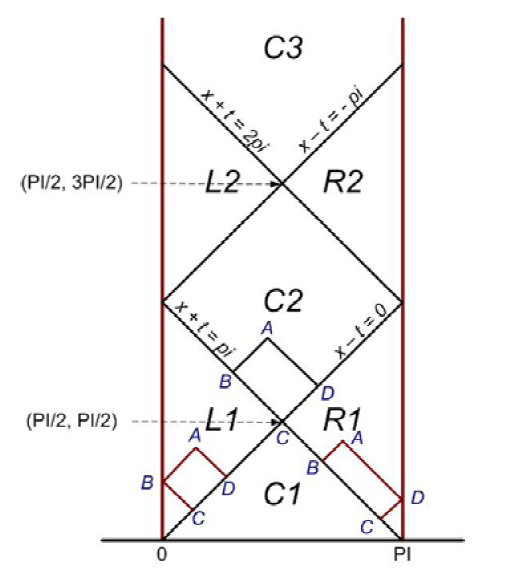
\includegraphics[width=0.7\textwidth]{Region.png}
 \end{figure}

\newpage
In region $C1$, the solution $u$ is defined by d\textsc{\char13}Alembert\textsc{\char13}s formula and the solution is

$$u(x,t)=\frac{1}{2}(0+0)+\frac{1}{2}\int_{x-t}^{x+t}1\cdot d\xi= t.$$

In region $L1$, let $A=(x,t)$ in $L1$ and thus $B=(0,t-x)$, $C=(\dfrac{t-x}{2}, \dfrac{t-x}{2})$, and $D=(\dfrac{x+t}{2}, \dfrac{x+t}{2})$. Using the parallelogram rule, we find that $u(x,t)=u(D_{C1})-u(C_{C1})=\dfrac{x+t}{2} - \dfrac{t-x}{2}=x$.

In region $R1$, let $A=(x,t)$ in $R1$ and thus $B=(\dfrac{\pi + x -t}{2},\dfrac{\pi - x +t}{2})$, $C=(\dfrac{3\pi -x -t}{2}, \dfrac{x+t - \pi}{2})$, and $D=(\pi, \dfrac{x+t-\pi}{2})$. Using the parallelogram rule, we find that $u(x,t)=u(B_{C1})-u(C_{C1}) =$ $\dfrac{\pi-x+t}{2} - \dfrac{x+t-\pi}{2}=\pi - x$.

In region $C2$, let $A=(x,t)$ in $C2$ and thus $B=(\dfrac{\pi + x -t}{2},\dfrac{\pi - x +t}{2})$, $C=(\dfrac{\pi}{2}, \dfrac{\pi}{2})$, and $D=(\dfrac{x+t}{2}, \dfrac{x+t}{2})$. Using the parallelogram rule, we find that $u(x,t)=u(B_{L1})+u(D_{R1})-u(C_{C1})=\dfrac{\pi + x -t}{2} + \pi - \dfrac{x+t}{2} -\dfrac{\pi}{2}=\pi - t$.

\textbf{3.1.3} Consider the initial/boundary value problem:

\[
  \begin{cases}
  u_{tt}-u_{xx}=0,  &\text{for $0<x<\pi$ and $t>0$}, \\
  u(x,0)=x, u_t(x,0)=0, & \text{for $0<x<\pi$}, \\
  u_x(0,t)=0, u_x(\pi,t)=0, & \text{for $t\geq0$}.
  \end{cases}
\]

\begin{enumerate}[label=(\alph*)]
    \item Find a Fourier series solution, and sum the series in regions bounded by characteristics. Do you think that the solution is unique?
\end{enumerate}

We first want to find a Fourier series solution. We need to find $u(x,t)$ in the form

$$u(x,t)=\frac{a_0(t)}{2}+\sum_{n=1}^{\infty}a_n(t)\cos(nx)+\sum_{n=1}^{\infty}b_n(t)\sin(nx),$$

where $a_n(t)$ and $b_n(t)$ are determined by the boundary conditions. Hence,

$$u_x(x,t)=\sum_{n=1}^{\infty}-na_n(t)\sin(nx)+n b_n(t)\cos(nx),$$
$$u_x(x,0)=\sum_{n=1}^{\infty}n b_n(t)=0.$$

Therefore, $b_n(t)=0$ for every $n$. So, we can rewrite $u(x,t)$ as

$$u(x,t)=\frac{a_0(t)}{2}+\sum_{n=1}^{\infty}a_n(t)\cos(nx).$$

The partial differential equation is given as $u_{tt}-u_{xx}=0$. If we substitute $u(x,t)$ and solve through separation of variables we find that the functions $a_0(t)$ and $a_n(t)$ must satisfy the ordinary differential equations $a_0''(t)=0$ and $a_n''(t)+n^2a_n(t)=0$. The general solution to these equations are

$$a_0(t)=c_0(t)+d_0,$$
$$a_n(t)=c_n\sin(nt)+d_n\cos(nt).$$

If we differentiate both of these equations we will find that

$${a'_0}(t)=c_0,$$
$${a'_n}(t)=nc_n\cos(nt)-n d_n\sin(nt).$$

We can now use our remaining initial conditions to solve for $c_n$ and $d_n$. As $u(x,0)=x$ we have that

$$u(x,0)=\frac{a_0(0)}{2}+\sum_{n=1}^{\infty}a_n(0)\cos(nx)=\frac{d_0}{2}+\sum_{n=1}^{\infty}d_n\cos(nx)=x,$$

and as $u_t(x,0)=0$ we have that

$$u_t(x,t)=\frac{{a'_0}(t)}{2} + \sum_{n=1}^{\infty}{a'_n}(t)\cos(nx),$$
$$u_t(x,0)=\frac{{a'_0}(0)}{2} + \sum_{n=1}^{\infty}a'_n(0)\cos(nx)=\frac{c_0}{2}+\sum_{n=1}^{\infty}nc_n\cos(nx)=0.$$

Integrating and multiplying by $\cos(mx)$ produces

$$d_0=\pi,~~~ d_n=\frac{2}{\pi n^2}(\cos(n\pi) -1),~~~c_n=0. $$

Therefore, $a_0(t)=d_0=\pi$ and $a_n(t)=d_n\cos(nt)=\dfrac{2}{\pi n^2}(\cos(n\pi) -1)\cos(nt)$. Hence,

$$u(x,t)=\frac{a_0(t)}{2}+\sum_{n=1}^{\infty}a_n(t)\cos(nx)=\frac{\pi}{2}+\frac{2}{\pi}\sum_{k=1}^{\infty}\frac{(\cos(k\pi)-1)}{k^2}\cos(kt)\cos(kx).$$

\textbf{3.1.4} Consider the initial boundary value problem:

\[
  \begin{cases}
  u_{tt}-c^2 u_{xx}=0,  &\text{for $x,t>0$}, \\
  u(x,0)=g(x), u_t(x,0)=h(x), & \text{for $x>0$}, \\
  u(0,t)=0,  & \text{for $t\geq0$},
  \end{cases}
\]

where $g(0)=0=h(0)$. If we extend $g$ and $h$ as odd functions on $-\infty<x<\infty$, show that d\textsc{\char13}Alembert\textsc{\char13}s formula (6) gives the solution.

We know that d\textsc{\char13}Alembert\textsc{\char13}s formula is

$$u(x,t)=\frac{1}{2}(g(x+ct)+g(x-ct)) + \frac{1}{2c}\int_{x-ct}^{x+ct}h(\xi)d\xi.$$

We are given that

$$u(x,0)=\frac{1}{2}(g(x)+g(x)) + \frac{1}{2c}\int_{x}^{x}h(\xi)d\xi=g(x).$$

We can calculate $u_t(x,t)$ by the FTC to form

$$u_t(x,t)=\frac{1}{2}(cg'(x+ct)-cg'(x-ct)) + \frac{1}{2c}(ch(x+ct)+ch(x-ct)),$$
$$u_t(x,0)=\frac{1}{2}(cg'(x)-cg'(x)) + \frac{1}{2c}(ch(x)+ch(x))=h(x),$$

where

$$u(0,t)=\frac{1}{2}(g(ct)+g(-ct))+\frac{1}{2c}\int_{-ct}^{ct}h(\xi)d\xi.$$

As $g(x)$ and $h(x)$ are odd functions we have that $g(-ct)=-g(ct)$. Hence,

$$u(0,t)=\frac{1}{2}(g(ct)+g(-ct))+\frac{1}{2c}\int_{-ct}^{ct}h(\xi)d\xi=0.$$

Where we can calculate further derivatives by

$$u_{tt}(x,t)=\frac{1}{2}(c^2g''(x+ct)+c^2g''(x-ct)) + \frac{1}{2}(ch'(x+ct)-ch'(x-ct)),$$
$$u_x(x,t)=\frac{1}{2}(g'(x+ct)+g'(x-ct)) + \frac{1}{2c}(h(x+ct)-h(x-ct)),$$
$$u_{xx}(x,t)=\frac{1}{2}(g''(x+ct)+g''(x-ct)) + \frac{1}{2c}(h'(x+ct)-h'(x-ct)).$$

Thus, $u_{tt}-c^2u_{xx}=0$ and d\textsc{\char13}Alembert\textsc{\char13}s formula (6) gives the solution.

\textbf{3.1.6} Solve the initial/boundary value problem:

\[
  \begin{cases}
  u_{tt}-u_{xx}=1,  &\text{for $0<x<\pi$ and $t>0$}, \\
  u(x,0)=0, u_t(x,0)=0, & \text{for $0<x<\pi$}, \\
  u(0,t)=0, u(\pi,t)=-\pi^2/2, & \text{for $t\geq0$}.
  \end{cases}
\]

Describe the singularities (i.e., is $u$ $C^2$? If not, where does it fail? Is $u$ $C^1$? etc.)

We should first find a particular solution of the nonhomogeneous equation. This particular solution will reduce the problem to a boundary value problem for the homogeneous equation (as in 3.1.2 and 3.1.3).

Let\textsc{\char13}s find a particular solution. We will use a method similar to separation of variables. Assume that

$$u_p(x,t)=X(x).$$

Then, substituting into the PDE forms

$$-X''(x)=1 ~~~\implies~~~ X''(x)=-1.$$

We can integrate twice to find the solution of the PDE. The solution is

$$X(x)=-\frac{x^2}{2}+ax+b.$$

The boundary conditions form

$$u_p(0,t)=b=0,$$
$$u_p(\pi,t)=-\frac{(-\pi)^2}{2}+a\pi+b=\frac{-\pi^2}{2}~~~\implies~~~ a=0.$$

Hence, $a=b=0$ and the particular solution is

$$u_p(x,t)=-\frac{x^2}{2}.$$

The particular solution solves

\[
  \begin{cases}
  u_{p_{tt}}-u_{p_{xx}}=1,  &\text{for $0<x<\pi$ and $t>0$}, \\
  u_p(x,0)=-{x^2}/{2}, u_{p_t}(x,0)=0, & \text{for $0<x<\pi$}, \\
  u_p(0,t)=0, u_{p}(\pi,t)=-\pi^2/2, & \text{for $t\geq0$}.
  \end{cases}
\]

Next, we need to find a solution to the boundary value problem of the homogeneous equation

\[
  \begin{cases}
  u_{tt}-u_{xx}=0,  &\text{for $0<x<\pi$ and $t>0$}, \\
  u(x,0)={x^2}/{2}, u_t(x,0)=0, & \text{for $0<x<\pi$}, \\
  u(0,t)=0, u(\pi,t)=0, & \text{for $t\geq0$}.
  \end{cases}
\]

We can solve this through separation of variables. In fact, it is identical to 3.1.2 with $u(x,0)=1$ replaced by $u(x,0)={x^2}/{2}$.

Looking back to our solution of 3.1.2, we see that we need to change the initial condition for $c_n$ to

$$u_t(x,0)=\sum_{n=1}^{\infty}nc_n\sin(nx)=\frac{x^2}{2},$$

which produces

$$c_n=\frac{2}{n\pi}}\int_0^{\pi}\frac{x^2}{2}\sin(nx)dx=\frac{(2-\pi^2n^2)\cos(n\pi)+2n\pi\sin(n\pi)-2}{\pi n^4},&~~~~~~\text{for every n}.$$

Hence, we can solve the homogeneous equation $u_h(x,t)$. The solution is

\begin{align*}
\begin{split}
u_h(x,t)&=\sum_{n=1}^{\infty}c_n\sin(nt)\sin(nx) \\
&=\sum_{n=1}^{\infty}\frac{(2-\pi^2n^2)\cos(n\pi)+2n\pi\sin(n\pi)-2}{\pi n^4}\sin(nt)\sin(nx).
\end{split}
\end{align*}

We can then find $u(x,t)$. We have that $u(x,t)=u_h(x,t)+u_p(x,t)$ and therefore

$$u(x,t)=\sum_{n=1}^{\infty}\frac{(2-\pi^2n^2)\cos(n\pi)+2n\pi\sin(n\pi)-2}{\pi n^4}\sin(nt)\sin(nx)-\frac{x^2}{2}.$$

\textbf{3.2.2} Find the solution of the initial value problem

\[
  \begin{cases}
  u_{tt}=u_{xx} + u_{yy} + u_{zz}, \\
  u(x,y,z,0)=x^2+y^2, ~u_t(x,y,z,0)=0,
  \end{cases}
\]

(a) by using (37) and (b) by using (39).

First, we will apply Kirchoff\textsc{\char13}s formula to find the solution. Letting $(\xi,\eta,\zeta)$ denote a point on the unit sphere $S^2\subset\mathbb R^3$ and $dS$ be the surface area element on $S^2$, we see that (as $h(x)=0)$)

\begin{align*}
\begin{split}
u(x,y,z,t)&=\frac{\partial}{\partial t}\Bigg(\frac{t}{4\pi}\int_{S^2}\Big[(x+t\xi)^2+(y+t\eta)^2\Big]dS\Bigg) \\ &=
\frac{\partial}{\partial t}\Bigg(\frac{t}{4\pi}\int_{S^2}\Big[x^2+2xt\xi+t^2\xi^2+y^2+2yt\eta+t^2\eta^2]dS\Bigg) \\ &=
\frac{\partial}{\partial t}\Bigg(\frac{t}{4\pi}\Big[4\pi(x^2+y^2)+2xt\int_{S^2}\xi dS + 2yt \int_{S^2}\eta dS + t^2\int_{S^2}\xi^2 dS +  t^2\int_{S^2}\eta^2 dS\Big]\Bigg).
\end{split}    
\end{align*}

Although,

$$\int_{S^2}\xi dS=0,$$

which can be verified through explicit calculation using spherical coordinates, or by symmetry (just split $S^2$ into the hemispheres $\xi\geq 0$ and $\xi\leq 0$. You will find that the two integrals cancel out). By the same reasoning, $\int_{S^2}\eta dS=0$. Therefore, by the rotational symmetry of the sphere we have that

$$\int_{S^2}\xi^2 dS=\int_{S^2}\eta^2 dS=\int_{S^2}\zeta^2 dS \implies \int_{S^2}\xi^2 dS=\frac{1}{3}\int_{S^2}(\xi^2+\eta^2+\zeta^2)dS=\frac{1}{3}\int_{S^2}dS=\frac{4\pi}{3}.$$

Hence, we can conclude that

$$u(x,y,z,t)=\frac{\partial}{\partial t}\Bigg(\frac{t}{4\pi}\Big[4\pi(x^2+y^2)+t^2\frac{8\pi}{3}\Big]\Bigg)=x^2+y^2+2t^2.$$

For (b), we need to use the 2d formula given in (39). This is possible since the data are independent of $z$. Let\textsc{\char13}s denote $(\xi,\eta)$ as a point on the unit disk $D = \{(\xi,\eta) : \xi^2 + \eta^2 < 1\}$ in the plane. Then (once again, $h(x)=0)$,

\begin{align*}
\begin{split}
u(x,y,z,t)&=\frac{\partial}{\partial t}\Bigg(\frac{t}{2\pi}\int_{D}\frac{(x+t\xi)^2+(y+t\eta)^2}{\sqrt{1-\xi^2-\eta^2}}d\xi d\eta\Bigg) \\ &=
\frac{\partial}{\partial t}\Bigg(\frac{t}{2\pi}\int_{D}\frac{x^2+y^2+2xt\xi+2yt\eta+t^2(\xi^2+\eta^2) }{\sqrt{1-\xi^2-\eta^2}}d\xi d\eta\Bigg) \\ &=
\frac{\partial}{\partial t}\Bigg(\frac{t}{2\pi}\Bigg[(x^2+y^2)\int_{D}\frac{d\xi d\eta}{\sqrt{1-\xi^2-\eta^2}}+2xt\int_{D}\frac{\xi d\xi d\eta}{\sqrt{1-\xi^2-\eta^2}}\\ 
&~~~~~~~~~+2yt\int_{D}\frac{\eta d\xi d\eta}{\sqrt{1-\xi^2-\eta^2}}+t^2\int_{D}\frac{(\xi^2+\eta^2) d\xi d\eta}{\sqrt{1-\xi^2-\eta^2}}\Bigg]\Bigg).
\end{split}    
\end{align*}

So, by symmetry

$$\int_{D}\frac{\xi d\xi d\eta}{\sqrt{1-\xi^2-\eta^2}}=\int_{D}\frac{\eta d\xi d\eta}{\sqrt{1-\xi^2-\eta^2}}=0.$$

Thus, if we switch to polar coordinates $(r,\theta)$ in the plane, we see that

$$\int_{D}\frac{d\xi d\eta}{\sqrt{1-\xi^2-\eta^2}}=\int_0^1\int_0^{2\pi}\frac{rdrd\theta}{\sqrt{1-r^2}}=2\pi\int_0^1\frac{rdr}{\sqrt{1-r^2}}=\pi\int_0^1\frac{ds}{\sqrt{s}}=2\pi,$$

and

$$\int_{D}\frac{(\xi^2+\eta^2) d\xi d\eta}{\sqrt{1-\xi^2-\eta^2}}=\int_0^1\int_0^{2\pi}\frac{r^2(rdrd\theta)}{\sqrt{1-r^2}}=2\pi\int_0^1\frac{r^3dr}{\sqrt{1-r^2}}=\pi\int_0^1\frac{(1-s)ds}{\sqrt{s}}=\frac{4\pi}{3}.$$

Hence, we can conclude that

$$u(x,y,z,t)=\frac{\partial}{\partial t}\Bigg(\frac{t}{2\pi}\Big[2\pi(x^2+y^2)+t^2\frac{4\pi}{3}\Big]\Bigg)=x^2+y^2+2t^2.$$

\textbf{3.2.3} Use Duhamel\textsc{\char13}s principle to find the solution of the nonhomogenuous wave equation for three space dimensions $u_{tt}-c^2\Delta u=f(x,t)$ with initial conditions $u(x,0)=0=u_t(x,0)$. What regularity in $f(x,t)$ is required for the solution $u$ to be $C^2$.

We are given the nonhomogeneous wave equation with the following initial conditions

\[
  \begin{cases}
  u_{tt}-c^2\Delta u=f(x,t), \\
  u(x,0)=0=u_t(x,0).
  \end{cases}
\]

By Duhamel\textsc{\char13}s principle, we reduce the problem to the special homogeneous equations with
nonhomogeneous initial conditions

\[
  \begin{cases}
  U_{tt}-c^2\Delta U=0, &\text{for $x\in\mathbb R$, $t>0$, $s\geq 0$},\\
  U(x,0,s)=0, &\text{for $x\in\mathbb R$, $s\geq 0$},\\
  U_t(x,0,s)=f(x,s), &\text{for $x\in\mathbb R$, $s\geq 0$}.
  \end{cases}
\]

Then, we have that

$$u(x,t)=\int_0^t U(x,t-s,s)ds,$$

solves the nonhomogeneous wave equation. With three spacial dimensions we can apply Kirchhoff\textsc{\char13}s formula (with $g(x)=0$ and $h(x)=f(x)$) to see that

$$U(x,t,s)=\frac{1}{4\pi}\frac{\partial}{\partial t}\Bigg(t\int_{|\xi|=1} 0 dS_{\xi}\Bigg) + \frac{t}{4\pi}\int_{|\xi|=1} f(x+ct\xi,s)dS_{\xi}=\frac{t}{4\pi}\int_{|\xi|=1} f(x+ct\xi,s)dS_{\xi}.$$

Therefore,

\begin{align*}
\begin{split}
u(x,t)=\int_0^t U(x,t-s,s)ds &= \int_0^t \Bigg(\frac{t-s}{4\pi}\int_{|\xi|=1} f(x+c(t-s)\xi,s)dS_{\xi} \Bigg)ds \\ &= \frac{1}{4\pi}\int_0^t\int_{|\xi|=1} (t-s)f(x+c(t-s)\xi,s)dS_{\xi} ds.
\end{split}
\end{align*}

Hence, we see that $f(x,t)$ needs to be $C^2$ in $x$ and $C^0$ in $t$ for the solution $u$ to be $C^2$.


\textbf{3.2.4} Let $\Omega=\{(x,y)\in\mathbb R^2 : \text{$0<x<a$ and $0<y<b$}\}$, and use separation of variables to solve the initial/boundary value problem

\[
  \begin{cases}
    u_{tt}=u_{xx}+u_{yy}, & \text{for $(x,y)\in\Omega$ and $t>0$}, \\
    u(x,y,t)=0, & \text{for $(x,y)\in\partial\Omega$ and $t>0$}, \\
    u(x,y,0)=\sin{\dfrac{\pi x}{a}}\sin{\dfrac{2\pi y}{b}}, ~\text{and}~u_t(x,y,0)=0, & \text{for $(x,y)\in\Omega$}.
  \end{cases}
\]

Letting $u(x,y,t)=X(x)Y(y)T(t)$, we form

$$XYT''=X''YT + XY''T.$$

If we divide every term by $XYT$, we get

$$\frac{T''}{T} = \frac{X''}{X} + \frac{Y''}{Y},$$

which must be equal to some constant $\lambda$. Therefore,

$$\frac{T''}{T} = \frac{X''}{X} + \frac{Y''}{Y} = - \lambda. $$

Then, acknowledging that $\frac{X''}{X}=-\mu^2, \frac{Y''}{Y}=-\nu^2$, and $\frac{T''}{T}=-\omega^2$ are constants, we see that

$$\lambda=\mu^2+\nu^2 + \omega^2.$$

Our initial condition tells us that

$$u(x,y,0)=\sin{\dfrac{\pi x}{a}}\sin{\dfrac{2\pi y}{b}}.$$

So, we know that

$$u(x,y,0)=X(x)Y(y)T(0)=\sin{\dfrac{\pi x}{a}}\sin{\dfrac{2\pi y}{b}}.$$

Hence, we need to find $T(t)$. Our initial conditions are

\[
  \begin{cases}
  T''+\omega^2 T=0, \\
  T(0)=\sin{\dfrac{\pi x}{a}}\sin{\dfrac{2\pi y}{b}},~~ T'(0)=0.
  \end{cases}
\]

Using these alongside the initial condition, $u(x,y,t)=0$, we find that

$$T(t)=\cos\bigg(\frac{\pi(4a^2+b^2)^{\frac{1}{2}}t}{ab}\bigg).$$

Therefore, our solution is

$$u(x,y,z)=X(x)Y(y)T(t)=sin{\dfrac{\pi x}{a}}\sin{\dfrac{2\pi y}{b}}\cos\bigg(\frac{\pi(4a^2+b^2)^{\frac{1}{2}}t}{ab}\bigg).$$

\textbf{3.2.5} Find a formula for the solution $v(x,t)=v(x_1,x_2,t)$ of the Cauchy problem for the two-dimensional Klein-Gordon equation:

\[
  \begin{cases}
  v_{tt}=c^2\Delta v - m^2v, ~~~ \text{for $x\in\mathbb R^2$ and $t>0$}, \\
  v(x,0)=g(x),~~~~~~v_t(x,0)=h(x).
  \end{cases}
\]

Using the hint in the back of the book, we define

$$u(x,y,z,t)=\cos\left(\frac{m}{c}z\right)v(x,y,t).$$

Where we can perform a calculation to see that $u$ satisfies the wave equation in 3d, so it is represented by Kirchhoff\textsc{\char13}s formula. Let's assume that $g=0$. Then, letting $(\xi,\eta,\zeta)$ denote a point on the unit sphere $S^2\subset\mathbb R^3$, we see that

$$u(x,y,z,t)=\frac{t}{4\pi}\int_{S^2}\cos\Big(\frac{m}{c}(z+ct\zeta)\Big)h(x+ct\xi,y+ct\eta)dS(\xi,\eta,\zeta).$$

If we let $z=0$, then

$$v(x,y,t)=u(x,y,0,t)=\frac{t}{4\pi}\int_{S^2}\cos(mt\zeta)h(x+ct\xi,y+ct\eta)dS(\xi,\eta,\zeta).$$

So, we now follow the derivation of the solution formula for the wave equation in 2d. We will parametrize the hemispheres $\zeta \geq 0$ and $\zeta \leq 0$ of $S^2$ as graphs

$$\zeta = \pm\sqrt{1-\xi^2-\eta^2},$$

over the unit disk $D = \{(\xi,\eta) : \xi^2 + \eta^2 \leq 1\}$. This will transform the integral to (observing that the cosine function is even, so there is no difference between the integrals in the two hemispheres)

$$v(x,y,t)=\frac{t}{2\pi}\int_D \frac{\cos\Big(mt\sqrt{1-\xi^2-\eta^2}\Big)h(x+ct\xi,y+ct\eta)}{\sqrt{1-\xi^2-\eta^2}}d\xi d\eta.$$

If we now remove the restriction that $g=0$, we can calculate the general form as
\begin{align*}
\begin{split}
v(x,y,t)=\frac{\partial}{\partial t}\Bigg(\frac{t}{2\pi}\int_D\frac{\cos\Big(mt\sqrt{1-\xi^2-\eta^2}\Big)g(x+ct\xi,y+ct\eta)}{\sqrt{1-\xi^2-\eta^2}}d\xi d\eta\Bigg) +\\ \frac{t}{2\pi}\int_D \frac{\cos\Big(mt\sqrt{1-\xi^2-\eta^2}\Big)h(x+ct\xi,y+ct\eta)}{\sqrt{1-\xi^2-\eta^2}}d\xi d\eta.
\end{split}
\end{align*}


\textbf{3.3.1} Let $\Omega$ be a smooth, bounded domain in $\mathbb R^n$. For a $C^2$ solution $u(x,t)$ of the wave equation $u_{tt}=c^2\Delta u$ for $x\in\Omega,t>0$, define the energy to be $\textepsilon_{\Omega}(t)=\frac{1}{2}\int_{\Omega}(u_t^2+c^2|\nabla u|^2)$ dx. If $u$ satisfies either the boundary condition $u(x,t)=0$ or $\partial u / \partial \nu(x,t)=0$ for $x\in\partial\Omega$, where $\nu$ is the exterior unit normal, then show that $\textepsilon_{\Omega}(t)$ is constant.

We consider solutions to the wave equation

$$u_{tt}=c^2\Delta u, ~~~~~u=u(x,t),  ~~~~~x\in\Omega,t>0,$$

which have a Dirichlet boundary condition

$$u(x,t)=0, ~~~~~\text{for all $x\in\partial\Omega,t\geq 0$},$$

or a Neumann boundary condition

$$\nabla u \cdot \nu = \frac{\partial u}{\partial \nu}(x,t)=0,~~~~~\text{for all $x\in\partial\Omega,t\geq 0$}.$$

We should assume that $u$ belongs to the space

$$u\in C^2(\overline{\Omega}\times(0,\infty))\cap C^1(\overline{\Omega}\times[0,\infty)).$$

We need to show that energy 

$$\textepsilon_{\Omega}(t)=\frac{1}{2}\int_{\Omega}(u_t^2+c^2|\nabla u|^2) ~dx,$$

is conserved. If we take the first derivative with respect to $t$, we find that

$$\frac{d}{dt}\textepsilon_{\Omega}(t)=\frac{d}{dt}\Bigg(\frac{1}{2}\int_{\Omega}(u_t^2+c^2|\nabla u|^2) ~dx\Bigg) =\int_{\Omega}(u_tu_{tt}+c^2\nabla u \cdot \nabla u_t)~ dx.$$

But, we know from Green's first identity that

$$\int_{\partial\Omega}v\frac{\partial u}{\partial \nu}dS = \int_{\Omega}(v \Delta u + \nabla v \cdot \nabla u)~dx.$$

Letting $v=u_t$, we see that

$$\int_{\Omega}\nabla u \cdot \nabla u_t ~dx = \int_{\partial\Omega}u_t\frac{\partial u}{\partial \nu}dS - \int_{\Omega}u_t\Delta u~ dx,$$

and the middle term vanishes because of the Dirichlet or Neumann boundary conditions. For the Neumann boundary condition, we have that $\frac{\partial u}{\partial \nu}=0$ on $\partial\Omega$. For the Dirichlet boundary condition, we have that $u=0$ on $\partial\Omega ~\implies$ $u_t=0$ on $\partial\Omega$. Hence, 

$$\int_{\Omega}\nabla u \cdot \nabla u_t ~dx =  - \int_{\Omega}u_t\Delta u~ dx,$$

and therefore

$$\frac{d}{dt}\textepsilon_{\Omega}(t)=\int_{\Omega}(u_tu_{tt}-c^2u_t\Delta u) ~dx= \int_{\Omega}u_t(u_{tt}-c^2\Delta u)~ dx=0.$$

Thus, energy is conserved.

\textbf{3.3.2} Use the previous exercise to show uniqueness of the solution for the (nonhomogenuous) wave equation $u_{tt}=\Delta u + f(x,t)$ in a smooth, bounded domain $\Omega\subset\mathbb R^n$ with either (a) Dirichlet condition $u=g$ on $\partial\Omega$, or (b) Neumann condition $\partial u/\partial \nu=h$ on $\partial\Omega$.

We need to prove uniqueness of solutions to the initial boundary value problem

\[
  \begin{cases}
  u_{tt}-c^2\Delta u=f(x,t), &\text{for $x\in\Omega$, $t>0$,} \\
  u(x,t)=\gamma(x,t), &\text{for $x\in\partial\Omega$, $t>0$}, \\
  u(x,0)=g(x), u_t(x,0)=h(x),& \text{for $x\in\Omega$}, 
  \end{cases}
\]

where $f ,\gamma, g ,h$ are given functions, and $u$ is assumed to belong to the space

$$u\in C^2(\Omega\times(0,\infty))\cap C^1(\overline{\Omega}\times[0,\infty)).$$

Let\textsc{\char13}s assume that $u,v$ both belong this space and solve the initial boundary value problem defined above. Then, $w=u-v$ also solves the initial boundary value problem with $f=0,$ $\gamma=0,$ $g=0$, and $h=0$. So, by the previous exercise, we see that the energy in $\Omega$ must be zero for all $t\geq 0$ as all of the functions are zero. Hence,

$$\textepsilon_{\Omega}(t)=\textepsilon_{\Omega}(0)=0.$$

Although, as $\textepsilon_{\Omega}(t)$ is defined by $\textepsilon_{\Omega}(t)=\frac{1}{2}\int_{\Omega}(w_t^2+c^2|\nabla w|^2)$ dx=0, it must be that $w_t=0$ and $\nabla w=0$ in $\Omega\times[0,\infty)$. Therefore, $w=\hspace{1mm}$constant and this constant must be zero as $w=0$ at time $t=0$. So, $w=0 ~\implies~ u=v$.

An analogous argument holds if we replace the Dirichlect boundary condition with the Neumann boundary condition.

\textbf{3.3.4} The partial differential equation $u_{tt}=c^2\Delta u -q(x)u$ arises in the study of wave propogation in a nonhomogenuous elastic medium: $q(x)$ is nonnegative and proportional to the coefficient of elasticity at $x$.

\begin{enumerate}[label=(\alph*)]
    \item Define an appropriate notion of energy for solutions.
    \item Verify the corresponding energy inequality.
    \item Use the energy method to prove that solutions are uniquely determined by their Cauchy data.
\end{enumerate}

(a) The energy integral is

$$\textepsilon(t)=\frac{1}{2}\int_{\Omega}(|u_t|^2+c^2|\nabla u|^2+q(x)u^2) dx.$$

We can verify this by differentiating with respect to $t$ to obtain

$$\frac{d}{dt}\textepsilon(t)=\frac{1}{2}\int_{\Omega}(u_tu_{tt}+c^2\sum_{i=1}^n u_{x_i}u_{x_i}t + q(x)uu_t) dx.$$

Integrating by parts then produces

$$\frac{d}{dt}\textepsilon(t)=\int_{\Omega}u_t\big(u_{tt}-c^2\Delta u +q(x)\big)dx=0,$$

which shows that $\textepsilon(t)$ must be a constant.

(b) For any time $\uptau\in[0,t_0]$, let $\overline{B}_{\uptau}=\{x\in\mathbb R^n:|x-x_0|\leq c(t_0-\uptau)\}$. Consider the local energy function

\begin{equation}
E_{x_0,t_0}(\uptau)=\frac{1}{2}\int_{B_{\uptau}}(u_t^2+c^2|\nabla u|^2+q(x)u^2)\big|_{t=\uptau}dx, ~~~~~~~\text{for $0\leq \uptau\leq t_0$}.
\end{equation}

We claim that (1) is a nonincreasing function of $\uptau$; that is, the following energy inequality holds:

\begin{equation}
E_{x_0,t_0}(\uptau)\leq E_{x_0,t_0}(0), ~~~~~~~\text{for $0\leq \uptau\leq t_0$}.
\end{equation}

To prove (2), we introduce the following notations

$$\Omega_{\uptau}=\{(x,t):|x-x_0|< c(t_0-t),0<t<\uptau\},$$
$$C_{\uptau}=\{(x,t):|x-x_0|= c(t_0-t),0<t<\uptau\}.$$

Notice that $\partial\Omega_{\uptau}=C_{\uptau}\cup(\overline{B}_0\times\{0\})\cup(\overline{B}_{\uptau}\times\{\uptau\})$, where the unions are disjoint. Moreover, the exterior unit normal $\nu$ on $\partial\Omega_{\uptau}$ is given on $\overline{B}_{\uptau}\times\{\uptau\}$ by $\nu=\langle 0,\dots,0,1 \rangle$, and on $\overline{B}_0$ by $\nu=\langle 0,\dots,0,-1 \rangle$. On $C_{\uptau}$, the normal $\nu=\langle \nu_1,\dots,\nu_n,\nu_{n+1} \rangle$ satisfies $c^2(\nu_1^2 + \cdots + \nu_n^2)=\nu_{n+1}^2$; together with the unit length condition $\nu_1^2 + \cdots + \nu_n^2 + \nu_{n+1}^2=1$, this implies

$$\nu_1^2 + \cdots + \nu_n^2=\frac{\nu_{n+1}^2}{c^2}=\frac{1}{1+c^2}.$$

Given a solution $u$, we define the vector field

$$\vec{V}=\langle 2c^2u_tu_{x_1},\dots,2c^2u_tu_{x_n},-(c^2|\nabla u|^2+u_t^2+q(x)u^2)\rangle.$$

If we calculate the divergence in $(x,t)$, we find

\begin{align*}
\begin{split}
\text{div} ~\vec{V}=2c^2(u_{tx_1}u_{x_1}+u_tu_{x_1x_1}+\cdots+u_{tx_n}u_{x_n}+u_tu_{x_nx_n})\\~-
        2c^2(u_{tx_1}u_{x_1}+\cdots+u_{tx_n}u_{x_n})-2u_tu_{tt}-2q(x)uu_t=0.
\end{split}
\end{align*}

The divergence theorem therefore implies

$$\int_{\partial\Omega_{\uptau}}\vec{V}\cdot\nu dS=0.$$

Now, on $C_{\uptau}$, the following inequality holds

$$2u_t(u_{x_1}\nu_1+\cdots+u_{x_n}\nu_n)\leq \frac{c}{\sqrt{1+c^2}}|\nabla u|^2 + \frac{1}{c\sqrt{1+c^2}}(u_t^2+q(x)u^2).$$

Therefore, we may compute on $C_{\uptau}$

$$\vec{V}\cdot\nu=2c^2u_t(u_{x_1}\nu_1+\cdots+u_{x_n}\nu_n)-(c^2|\nabla u|^2+{u_t}^2+q(x)u^2)\nu_{n+1}\leq 0,$$

so in particular

$$\int_{C_{\uptau}}\vec{V}\cdot\nu dS \leq 0.$$

Then, we have

\begin{align*}
\begin{split}
0 &\leq \int_{\overline{B}_0} \vec{V}\cdot\nu dS + \int_{\overline{B}_{\uptau}\times\{\uptau\}} \vec{V}\cdot\nu dS \\&=
\int_{\overline{B}_0}(c^2|\nabla u|^2+{u_t}^2+q(x)u^2)\big|_{t=0} dx - \int_{\overline{B}_{\uptau}} (c^2|\nabla u|^2+{u_t}^2+q(x)u^2)\big|_{t=\uptau} dx,
\end{split}
\end{align*}

which proves (2),

\begin{equation*}
E_{x_0,t_0}(\uptau)\leq E_{x_0,t_0}(0), ~~~~~~~\text{for $0\leq \uptau\leq t_0$}.
\end{equation*}

(c) Let both $u$ and $v$ be solutions to $u_{tt}=c^2\Delta u - q(x)u$ on $C^2(\Omega\times(0,\infty))$ with initial conditions $u(x,0)=g(x), u_t(x,0)=h(x)$ for $x\in\Omega$. Let $w\equiv u -v$, then

\[
  \begin{cases}
  w_{tt}=c^2\Delta w - q(x)w, &\text{for $x\in\Omega$, $t>0$}, \\
  w(x,0)=w_t(x,0)=0, &\text{for $x\in\Omega$} .
  \end{cases}
\]

Hence, we know that $\textepsilon(t)=\textepsilon(0)=0$. It follows that

$$\textepsilon(t)=\frac{1}{2}\int_{\Omega}(|w_t|^2+c^2|\nabla w|^2+q(x)w^2) dx=0,$$

since $q(x)$ is nonnegative and the third term implies that $w(x,t)\equiv 0$. Therefore, $u(x,t)\equiv v(x,t)$.

\textbf{4.1.1} Let $\Omega=\{(x,y)\in\mathbb R^2 : x^2+y^2<1\}=\{(r,\theta):0\leq r <1, 0 \leq \theta < 2\pi\}$, and use separation of the variables $(r,\theta)$ to solve the Dirichlet problem

\[
  \begin{cases}
  \Delta u = 0, & \text{in $\Omega$}, \\
  u(1,\theta) =g(\theta), & \text{for $0\leq \theta < 2\pi$}.
  \end{cases}
\]

It is natural to use polar coordinates $(r,\theta)$ in which the problem becomes

\[
  \begin{cases}
  \dfrac{\partial^2 u}{\partial r^2} + \dfrac{1}{r}\dfrac{\partial u}{\partial r} + \dfrac{1}{r^2}\dfrac{\partial^2 u}{\partial \theta^2}=0, & \text{for $0\leq r < 1$, $0\leq \theta < 2\pi$}, \\
  u(1,\theta) =g(\theta), & \text{for $0\leq \theta < 2\pi$}.
  \end{cases}
\]

If we write $r=e^{-t}$ ad $u(r,\theta)=X(t)Y(\theta)$, then

$$r^2\partial_r^2 u + r\partial_r u + \partial_{\theta}^2 u = \partial_t^2 u + \partial_{\theta}^2 u = X''(t)Y(\theta)+X(t)Y''(\theta)=0.$$

Separating the variables, we obtain

$$\frac{X''(t)}{X(t)}=-\frac{Y''(\theta)}{Y(\theta)}=\lambda.$$

But $Y''(\theta)+\lambda Y(\theta)=0$ has solutions $\lambda_n=n^2$ and $Y_n(\theta)=a_n\cos n\theta $ $+ b_n\sin n\theta$; notice $Y_0(\theta)=a_0=$const. The equation $X''(t)+n^2X(t)=0$ has solutions $X_0(t)=c_0 t + d_0$ and $X_n(t)=c_n e^{nt}+ d_n e^{-nt}$ for $n=1,2,3,\dots$ . This means that $u_0(r,\theta)=-c_0\log r + d_0$ and $u_n(r,\theta)=(a_n \cos n\theta + b_n\sin n\theta)$ $(c_n r^{-n} + d_n r^n)$ for $n=1,2,3,\dots$ . But $u$ must be finite at $r=0$, so $c_n=0$. By superposition we may write (after relabeling coefficients)

$$u(r,\theta)=a_0+\sum_{n=1}^{\infty}r^n(a_n \cos n\theta + b_n\sin n\theta).$$

But then

$$u(1,\theta)=a_0+\sum_{n=1}^{\infty}(a_n \cos n\theta + b_n\sin n\theta)=g(\theta),$$

which shows that the coefficients $a_n$,$b_n$ for $n\geq 1$ are determined from the Fourier series for $g(\theta)$. Therefore,

$$a_n=\frac{1}{\pi}\int_0^{2\pi}g(\theta)\cos(n\theta)d\theta &~~~~~ \text{for $n=1,2,3\dots$},$$
$$b_n=\frac{1}{\pi}\int_0^{2\pi}g(\theta)\sin(n\theta)d\theta&~~~~~ \text{for $n=1,2,3\dots$}.$$
Notice, however that $a_0$ is not determined by $g(\theta)$ and therefore may take any arbitrary value. Moreover, the constant term in the Fourier series for $g(\theta)$ must be zero. So, we can write

$$a_0=\frac{1}{2\pi}\int_0^{2\pi}g(\theta)d\theta.$$

\textbf{4.1.2} Let $\Omega=(0,\pi)\times(0,\pi)$, and use separation of variables to solve the mixed boundary value problem

\[
  \begin{cases}
  \Delta u = 0, & \text{in $\Omega$}, \\
  u_x(0,y)=0=u_x(\pi,y), & \text{for $0 < y < \pi$}, \\
  u(x,0)=0,~~ u(x,\pi)=g(x), & \text{for $0 < x < \pi$}.
  \end{cases}
\]

Assume $u(x,y)=X(x)Y(y)$. Substitution into the PDE produces

$$X''(x)Y(y)+X(x)Y''(y)=0.$$

Separating the variables, we obtain

$$\frac{X''(x)}{X(x)}=-\frac{Y''(y)}{Y(y)}=-\lambda.$$

For the first equation, consider $X''(x)+\lambda X(x)=0$. If $\lambda = 0$, then $X''(x)=0$ and we can simplify this to find $X_0(x)=a_0x + b_0$.

Else, if $\lambda \neq 0$ then we need to solve $X''(x)+\lambda X(x)=0$. By standard ODE techniques, we find that the roots of the characteristic polynomial are $r=\pm i\lambda$. Therefore, we see that $X_n(x)=a_n\cos nx + b_n\sin nx$.

The boundary conditions are $u_x(0,y)=0=u_x(\pi,y)$. So,

$$u_x(0,y)=X'(0)Y(y)=0 ~~~\implies~~X'(0)=0,$$
$$u_x(\pi,y)=X'(\pi)Y(y)=0 ~~~\implies~~X'(\pi)=0.$$

Hence, $X_0'(0)=a_0=0$ and $X_n'(0)=n b_n = 0 ~\implies~b_n=0$. Thus, $X_0(x)=b_0$ and $X_n(x)=a_n\cos nx$.

If we return back to our original equation $X''(x)+\lambda X(x)=0$, we can substitute in the above form to find that $-n^2 a_n \cos nx + \lambda a_n \cos nx = 0$. This implies that

$$\lambda = n^2 ~~~~~ &\text{for $n=1,2,3,\dots$ .}$$

So, we now consider $Y''(y)-\lambda Y(y)=0$ or $Y''(y)-n^2 Y(y)=0$. If $n=0$, then we have $Y''(y)=0$ and we can simplify this to find $Y_0(y)=c_0 y + d_0$.

Else, if $n \neq 0$ then we need to solve $Y''(y)-n^2 Y(y)=0$. By standard ODE techniques, we find that the roots of the characteristic polynomial are $r=\pm n$. Therefore, we see that $Y_n(y)=c_n e^{ny} + d_n e^{-ny}$.

The boundary condition is $u(x,0)=0$. So,

$$u(x,0)=0=X(x)Y(0)=0 ~~~\implies~~Y(0)=0.$$

Hence, $Y_0(0)=d_0=0$ and $Y_n(0)=c_n + d_n=0  ~\implies~c_n=-d_n$. Thus, $Y_0(y)=c_0y$ and $Y_n(y)=c_n(e^{ny}-e^{-ny})=\widetilde{c_n}\sinh ny$.

If we put everything together, we form

$$u_0(x,y)=X_0(x)Y_0(y)=b_0c_0 y = \widetilde{a_0} y,$$
$$u_n(x,y)=X_n(x)Y_n(y)=(a_n\cos nx)(\widetilde{c_n}\sinh ny) = \widetilde{a_n} \cos nx \sinh ny.$$

So, by superposition, we can write

$$u(x,y)=\widetilde{a_0} y + \sum_{n=1}^{\infty}\widetilde{a_n} \cos nx \sinh ny.$$

The above equation satisfies the three homogeneous boundary conditions. For the non-homogeneous boundary condition, we have that $u(x,\pi)=g(x)$. So,

$$u(x,\pi)=\widetilde{a_0} \pi + \sum_{n=1}^{\infty}\widetilde{a_n} \cos nx \sinh n\pi=g(x).$$

By the orthogonality conditions of coefficients, we have that

$$\int_0^{\pi}g(x)dx= \int_0^{\pi}(\widetilde{a_0} \pi + \sum_{n=1}^{\infty}\widetilde{a_n} \cos nx \sinh n\pi)dx = \widetilde{a_0} \pi^2 ~~\implies~~\widetilde{a_0}=\frac{1}{\pi^2}\int_0^{\pi}g(x)dx,$$

$$\int_0^{\pi}g(x)\cos mx ~dx= \sum_{n=1}^{\infty}\widetilde{a_n}\sinh  n\pi \int_0^{\pi}\cos nx \cos mx~dx=\frac{\pi}{2}\widetilde{a_m}\sinh m\pi,$$

which implies that

$$\widetilde{a_n}\sinh n\pi=\frac{2}{\pi}\int_0^{\pi}g(x)\cos nx ~dx.$$


\textbf{4.1.3} Prove that the solution of the Robin or third boundary value problem (5) for the Laplace equation is unique when $\alpha>0$ is a constant.

We have that

\[
  \begin{cases}
  \Delta u = 0, & \text{in $\Omega$}, \\
  \frac{\partial u}{\partial \nu} + \alpha u =\beta, & \text{on $\partial \Omega$},
  \end{cases}
\]

where $\alpha, \beta$ are constants with $\alpha > 0$. We need to prove uniqueness. Assume that

$$u,v \in C^2(\Omega)\cap C^1(\overline{\Omega}),$$

are both solutions to the Laplace equation. Let $w=u-v$. Then, w satisfies

\[
  \begin{cases}
  \Delta w = 0, & \text{in $\Omega$}, \\
  \frac{\partial w}{\partial \nu} + \alpha w =0, & \text{on $\partial \Omega$}.
  \end{cases}
\]

If we apply Green's first identity with $u,v=w$, we find that 

$$\int_{\partial\Omega} w \frac{\partial w}{\partial \nu}dS=\int_{\Omega}\nabla w \cdot \nabla w~dx=\int_{\Omega}|\nabla w|^2 dx.$$

If we now insert the boundary conditions, $\dfrac{\partial w}{\partial \nu} = -\alpha w$ on $\partial\Omega$, we find that

$$-a\int_{\partial\Omega} w^2 dS=\int_{\Omega}|\nabla w|^2 dx.$$

Therefore, in the formula above the LHS is always $\leq 0$ while the RHS is always $\geq 0$. So, both sides must equal zero. Hence, $w=0$ in $\Omega$. As we assumed that $w$ is continuous on the boundary, we also have that $w=0$ in $\overline{\Omega}$. Thus, u=v.

\textbf{4.1.4} Let $\Omega$ be the unit disk as in Exercise 1.
\begin{enumerate}[label=(\alph*)]
    \item Solve the Robin problem (5) for the Laplace equation when $\alpha > 0$ is constant.
\end{enumerate}

We are given that the solution by separation of variables on the unit disk is

$$u(r,\theta)=a_0+\sum_{n=1}^{\infty}r^n(a_n \cos n\theta + b_n\sin n\theta),$$

where the normal derivative on the boundary can be represented as

$$u_r(1,\theta)=\sum_{n=1}^{\infty}n(a_n \cos n\theta + b_n\sin n\theta).$$

So, we need to consider the new boundary condition of 

$$\frac{\partial u}{\partial \nu} + \alpha u =\beta, & ~~~~~\text{on $\partial \Omega$}.$$

Through this new boundary condition, we can write the equation above as

$$\beta(\theta)=\alpha a_0+\sum_{n=1}^{\infty}(\alpha+ n)(a_n \cos n\theta + b_n\sin n\theta).$$

Therefore, through the above representation we can find the Fourier coefficients as

$$\alpha a_0=\frac{1}{\pi}\int_{-\pi}^{\pi}\beta(\theta)d\theta ~~\implies~~ a_0=\frac{1}{\alpha\pi}\int_{-\pi}^{\pi}\beta(\theta)d\theta,$$

$$(\alpha+ n) a_n=\frac{1}{2\pi}\int_{-\pi}^{\pi}\beta(\theta)\cos(n\theta)d\theta ~~\implies~~ a_n=\frac{1}{2\pi(\alpha+ n)}\int_{-\pi}^{\pi}\beta(\theta)\cos(n\theta)d\theta,$$

$$(\alpha+ n) b_n=\frac{1}{2\pi}\int_{-\pi}^{\pi}\beta(\theta)\sin(n\theta)d\theta ~~\implies~~ b_n=\frac{1}{2\pi(\alpha+ n)}\int_{-\pi}^{\pi}\beta(\theta)\sin(n\theta)d\theta.$$

As $\alpha > 0$, it is clear that all of the Fourier coefficients for $a_0$, $a_n$, and $b_n$ are well defined. They are all determined uniquely and produce a unique solution.

\begin{enumerate}[label=(\alph*),start=2]
    \item When $\alpha=-1$, show that uniqueness fails.
\end{enumerate}

Consider

$$u(r,\theta)=r(a\sin(\theta)+b\cos(\theta)),$$

with the boundary condition

$$\frac{\partial u}{\partial \nu} + \alpha u =\beta, & ~~~~~\text{on $\partial \Omega$}.$$

The normal derivative on the boundary is

$$u_r(1,\theta)=(a\sin(\theta)+b\cos(\theta)).$$

So, the boundary condition becomes $\dfrac{\partial u}{\partial \nu} - u=0$. For $u(r,\theta)=r(a\sin(\theta)$ $+b\cos(\theta))$, we have that

\[
  \begin{cases}
  \Delta u = 0, & \text{in $\Omega$}, \\
  \frac{\partial u}{\partial \nu} - u =0, & \text{on $\partial \Omega$}.
  \end{cases}
\]

Therefore, we can no longer apply the same strategy used in (a). As $a$ and $b$ are arbitrary, there are many different values of $a$ and $b$ which satisfy both conditions. Hence, uniqueness fails.


\textbf{4.1.5} Suppose $q(x)\geq 0$ for $x\in\Omega$ and consider solutions $u\in C^2(\Omega)\cap C^1(\overline{\Omega})$ of $\Delta u - q(x)u=0$ in $\Omega$. Establish uniqueness theorems for (a) the Dirichlet problem, and (b) the Neumann problem.

Let's consider

$$\Delta u - q(x)u=0, & ~~~~~~\text{in $\Omega$},$$

where $q(x)\geq 0$ is assumed to be bounded and continuous in $\Omega$. If we also assume that $q(x)$ is not everywhere 0, then there exists a point $x_0\in\Omega$ such that

$$q(x_0)>0.$$

We need to prove uniqueness of solutions in the space

$$C^2(\Omega)\cap C^1(\overline{\Omega}),$$

subject to the two boundary conditions

$$u=g, ~~~~~~\text{on $\partial\Omega$},$$
$$\frac{\partial u}{\partial \nu}=h, ~~~~~~\text{on $\partial\Omega$},$$

where the Neumann boundary condition isn't unique if $q=0$. So, we assume that $q(x)$ is not everywhere zero.

Next, assume that $u,v$ are two solutions such that $u,v\in C^2(\Omega)\cap C^1(\overline{\Omega})$. Let $w=u-v$. Then, $w=u-v$ satisfies the original equation with the new boundary conditions

$$w=0, ~~~~~~\text{on $\partial\Omega$},$$
$$\frac{\partial w}{\partial\nu}=0, ~~~~~~\text{on $\partial\Omega$}.$$

In either case, we have that

$$\int_{\partial\Omega}w\frac{\partial w}{\partial \nu}dS=0.$$

So, if we apply Green's first identity with $u,v=w$ and $\Delta w = wq(x)$ we form

$$0=\int_{\partial\Omega}w\frac{\partial w}{\partial \nu}dS=\int_{\Omega}}w^2q(x)+ |\nabla w|^2~dx.$$

But, the integrand on the RHS is continuous and $\geq 0$, so we must have that $w^2q(x)+ |\nabla w|^2=0$ in $\Omega$. This means that

$$|\nabla w|^2=0 ~~\implies~~ \nabla w = 0 ~~\implies~~ w=\text{constant}=c, ~~~~~\text{in $\Omega$},$$
$$w^2q(x)=0 ~~\implies~~ \text{at $x=x_0$, $q(x_0)>0$} ~~\implies~~ w=0, ~~~~~\text{in $\Omega$}.$$

Therefore, as $w=0$ and $w=constant=c$ in $\Omega$ $~~\implies~~ c=0 ~~\implies~~w=0$ in $\Omega$. By continuity, we can also extend this to $\overline{\Omega}$. Hence, $u=v$ and we have established uniqueness for the Dirichlet and Neumann problem.

\textbf{4.1.6} By direct calculation, show that $v(x)=|x-x_0|^{2-n}$ is harmonic in $\mathbb R^n\setminus\{x_0\}$ for $n\geq 3$. Do the same for $v(x)=\log |x-x_0|$ if $n=2$.

Assume $n\geq 3$, fix $a\in\mathbb R^n$, and set $v(x)=|x-a|^{2-n}$ for $x\neq a$.

Then, $v(x)=r^{2-n}$ where

$$r=|x-a|=\sqrt{(x_1-a_a)^2+(x_2-a_2)^2+\cdots + (x_n-a_n)^2}.$$

Therefore,

$$r_{x_i}=\dfrac{2(x_i-a_i)}{2\sqrt{(x_1-a_a)^2+(x_2-a_2)^2+\cdots + (x_n-a_n)^2}}=\dfrac{x_i-a_i}{r}.$$

Hence, by the chain rule,

$$v_{x_i}=(2-n)r^{1-n}r_{x_i}=(2-n)r^{1-n}\dfrac{x_i-a_i}{r}=(2-n)r^{-n}(x_i-a_i),$$

and

\begin{equation*}
\begin{split}
v_{x_ix_i}&=(-n)(2-n)r^{-n-1}(x_i-a_i)r_{x_i}+(2-n)r^{-n}\\&=(-n)(2-n)r^{-n-1}(x_i-a_i)\dfrac{x_i-a_i}{r}+(2-n)r^{-n}\\&=
(-n)(2-n)r^{-n-2}(x_i-a_i)^2+(2-n)r^{-n}.
\end{split}
\end{equation*}

Thus,

\begin{equation*}
\begin{split}
\Delta v = \sum_{i=1}^n v_{x_ix_i}&=(-n)(2-n)r^{-n-2}r^2+n(2-n)r^{-n}\\&=
(n^2-2n)r^{-n}+(-n^2+2n)r^{-n}\\&=0.
\end{split}
\end{equation*}

Next, consider $n= 2$, fix $a\in\mathbb R^2$, and set $v(x)=\log|x-a|$ for $x\neq a$. Then, $v(x)=\log(r)$ where

$$r=|x-a|=\sqrt{(x_1-a_1)^2+(x_2-a_2)^2}.$$

Therefore,

$$r_{x_i}=\dfrac{2(x_i-a_i)}{2\sqrt{(x_1-a_1)^2+(x_2-a_2)^2}}=\dfrac{x_i-a_i}{r}.$$

So, by the chain rule,

$$v_{x_i}=\dfrac{1}{r}r_{x_i}=\dfrac{x_i-a_i}{r^2}=(x_i-a_i)r^{-2},$$

and

\begin{equation*}
\begin{split}
v_{x_ix_i}&=r^{-2}-2(x_i-a_i)r^{-3}r_{x_i} \\&=
\dfrac{1}{r^2}-\dfrac{2(x_i-a_i)}{r^3}\dfrac{(x_i-a_i)}{r}  \\&=
\dfrac{1}{r^2}-\dfrac{2(x_i-a_i)^2}{r^4}.
\end{split}
\end{equation*}

Thus,

\begin{equation*}
\begin{split}
\Delta v = \sum_{i=1}^2 v_{x_ix_i}&=2\dfrac{1}{r^2}-\dfrac{2r^2}{r^4}\\&=
\dfrac{2}{r^2} - \dfrac{2}{r^2} \\&=0.
\end{split}
\end{equation*}

\textbf{4.1.7}
\begin{enumerate}[label=(\alph*)]
    \item If $\Omega$ is a bounded domain and $u\in C^2(\Omega)\cap C(\overline\Omega)$ satisfies (1), then $\max_{\overline\Omega}|u| =\max_{\partial\Omega}|u|$.
\end{enumerate}

Assume that $u\in C^2(\Omega)\cap C(\overline\Omega)$ and that $\Delta u = 0$ in $\Omega$. We need to show that

$$\underset{\overline\Omega}{\max}|u| =\underset{\partial\Omega}{\max}|u|.$$

Observe that this is the same as the standard weak maximum principle where $u$ is replaced by $|u|$. Assume that $\Omega$ is bounded. We first need to show that

$$\underset{\overline\Omega}{\max}|u| \geq\underset{\partial\Omega}{\max}|u|.$$

But, this is obvious since ${\overline\Omega}$ contains ${\partial\Omega}$. So, we need to show that

$$\underset{\overline\Omega}{\max}|u| \leq\underset{\partial\Omega}{\max}|u|.$$

As $|u|$ is continuous and ${\overline\Omega}$ is a compact set, we know that $|u|$ must obtain a maximum. Therefore, $\exists ~x_1\in\overline\Omega}$ such that

$$|u(x_1)|=\underset{\overline\Omega}{\max}|u|.$$

WLOG, we may assume that $u(x_1)\geq 0$ (otherwise, if $u(x_1)\leq 0$, then we could replace u by -u). Thus,

$$u(x_1)=\underset{\overline\Omega}{\max}|u|.$$

As $u(x_1)\geq 0$, this implies that $\max_{\overline\Omega}u =\max_{\overline\Omega}|u|$. We know from the standard weak maximum principle that

$$\underset{\overline\Omega}{\max}~u =\underset{\partial\Omega}{\max}~u.$$

Therefore, we see that

$$\underset{\overline\Omega}{\max}|u|=u(x_1)=\underset{\overline\Omega}{\max}~u=\underset{\partial\Omega}{\max}~u\leq \underset{\partial\Omega}{\max}|u|.$$

Thus, $\underset{\overline\Omega}{\max}|u| \leq\underset{\partial\Omega}{\max}|u|$ and we have that $\max_{\overline\Omega}|u| =\max_{\partial\Omega}|u|$.

\begin{enumerate}[label=(\alph*),start=2]
    \item If $\Omega=\{x\in\mathbb R^n : |x| > 1\}$ and $u\in C^2(\Omega)\cap C(\overline\Omega)$ satisfies (1) and $\lim_{|x|\to\infty}u(x)=0$, then $\max_{\overline\Omega}|u| =\max_{\partial\Omega}|u|$.
\end{enumerate}

Assume that $u\in C^2(\Omega)\cap C(\overline\Omega)$, $\Delta u = 0$ in $\Omega$, and $\lim_{|x|\to\infty}u(x)=0$. Also assume that 

$$\Omega=\{x\in\mathbb R^n : |x| > 1\},$$

which is an unbounded set. We need to show that

$$\underset{\overline\Omega}{\max}|u| =\underset{\partial\Omega}{\max}|u|.$$

Similar to (a), it is obvious that $\max_{\overline\Omega}|u| \geq \max_{\partial\Omega}|u|$. So, we need to prove that

$$\underset{\overline\Omega}{\max}|u| \leq\underset{\partial\Omega}{\max}|u|.$$

To do this, let's split up the set into $\partial\Omega=\{x\in\mathbb R^n : |x| = 1\}$ and $\overline\Omega=\{x\in\mathbb R^n : |x| \geq 1\}$.

For $\partial\Omega=\{x\in\mathbb R^n : |x| = 1\}$, it is clear that the maximum is obtained. This set is compact, so we can repeat the argument used in part (a). For $\overline\Omega=\{x\in\mathbb R^n : |x| \geq 1\}$, we need to do something different. This set is unbounded, so we will need a different approach of attack.

On $\overline\Omega=\{x\in\mathbb R^n : |x| \geq 1\}$, assume that $u$ is not everywhere zero. If $u$ was everywhere zero, then we would have nothing to prove. Let

$$M:=\underset{\overline\Omega}{\sup}|u|>0.$$

As $\lim_{|x|\to\infty}u(x)=0$, there must exist a $R>0$ such that

$$|x|\geq R ~~~\implies~~~|u(x)|\leq \frac{M}{2}.$$

Define

$$B_R:=\{x : 1\leq|x| \leq R\}.$$

Then, $B_R$ is compact. So, the maximum of $|u|$ is obtained. Therefore, $\exists~x_1\in B_R$ such that $|u(x_1)|=\max_{B_R}|u|$. But, as $|x|\geq R ~\implies~|u(x)|\leq \frac{M}{2}$, we see that 

$$M=\underset{\overline\Omega_R}{\max}|u|.$$

Thus, the sup of $|u|$ over ${\overline\Omega}$ is the maximum. Hence,

$$|u(x_1)|=\underset{B_R}{\max}|u|=\underset{\overline\Omega}{\max}|u|.$$

Analogous to part (a), we may assume that WLOG $u(x_1)\geq 0$. Then,

$$u(x_1)=\underset{B_R}{\max}|u|=\underset{\overline\Omega}{\max}|u|.$$

So, from from the standard weak maximum principle in $B_R$, we know that

$$\underset{B_R}{\max}~u=\underset{\partial\Omega}{\max}~u,$$

which allows to conclude that

$$\underset{\overline\Omega}{\max}|u|=u(x_1)=\underset{B_R}{\max}~u=\underset{\partial\Omega}{\max}~u\leq \underset{\partial\Omega}{\max}|u|.$$

Thus, $\underset{\overline\Omega}{\max}|u| \leq\underset{\partial\Omega}{\max}|u|$ and we have that $\max_{\overline\Omega}|u| =\max_{\partial\Omega}|u|$.

\textbf{4.2.1} 
\begin{enumerate}[label=(\alph*)]
    \item If $n=2$ and $a=1$, show that (44) is equivalent to
\end{enumerate}

$$u(r,\theta)=\frac{1-r^2}{2\pi}\int_0^{2\pi}\frac{g(\phi)d\phi}{1+r^2-2r\cos(\theta-\phi)}.$$

The Poisson integral formula is given by

$$u(\xi)=\frac{a-|\xi|^2}{a\omega_n}\int_{|x|=a}\frac{g(x)}{|x-\xi|^n}dS_x.$$

Replacing $n=2$ and $a=1$, we have that $\omega_n=2\pi$ and thus

$$u(\xi)=\frac{1-|\xi|^2}{2\pi}\int_{|x|=1}\frac{g(x)}{|x-\xi|^2}dS_x.$$

But, this is the same as integrating over a circle of radius 1. Therefore,

$$u(\xi)=\frac{1-r^2}{2\pi}\int_0^{2\pi}\frac{g(\phi)}{|x-\xi|^2}d\phi,$$

where we set $\xi=(r\cos\theta,r\sin\theta)$ and $x=(\cos\phi,\sin\phi)$ to form

\begin{equation*}
\begin{split}
|x-\xi|^2&=|(r\cos\theta-\cos\phi,r\sin\theta-\sin\phi)|^2 \\&=
r^2\cos^2\theta-2r\cos\theta\cos\phi+\cos^2\phi + r^2\sin^2\theta-2r\sin\theta\sin\phi+\sin^2\phi \\&=
r^2(\cos^2\theta+\sin^2\theta)+(\cos^2\phi+\sin^2\phi)-2r(\cos\theta\cos\phi+\sin\theta\sin\phi) \\&=
r^2+1-2r(\cos(\theta-\phi)).
\end{split}
\end{equation*}

Therefore,

$$u(\xi)=\frac{1-r^2}{2\pi}\int_0^{2\pi}\frac{g(\phi)d\phi}{1+r^2-2r\cos(\theta-\phi)}.$$

\begin{enumerate}[label=(\alph*),start=2]
    \item Use (a) and Exercise 1 in Section 4.1 to verify the formula
\end{enumerate}

$$r^k\cos k\theta=\frac{1-r^2}{2\pi}\int_0^{2\pi}\frac{\cos (k\phi)d\phi}{1+r^2-2r\cos(\theta-\phi)},$$

where $k$ is an integer and $0\leq r < 1$.

We have that $g(\theta)$ is the boundary condition of the PDE. So, we want to find a function $u(r,\theta)$ solving

\[
  \begin{cases}
  \Delta u = 0, & \text{in $\Omega$}, \\
  u(1,\theta) =g(\theta), & \text{for $0\leq \theta < 2\pi$}.
  \end{cases}\tag{*}
\]

The function $u$ given by the Poisson formula is the unique solution to the problem, so if we have any function solving $(*)$, then that function must be equal to the Poisson integral.

In particular, from Exercise 1 in Section 4.1 we have that

\[
  \begin{cases}
  \dfrac{\partial^2 u}{\partial r^2} + \dfrac{1}{r}\dfrac{\partial u}{\partial r} + \dfrac{1}{r^2}\dfrac{\partial^2 u}{\partial \theta^2}=0, & \text{for $0\leq r < 1$, $0\leq \theta< 2\pi$}, \\
  u(1,\theta) =g(\theta)=\cos(k\theta), & \text{for $0\leq \theta < 2\pi$}.
  \end{cases}
\]

Substituting $u(r,\theta) = r^k \cos(k\theta)$, we see that it satisfies both of the hypothesis as

$$u_{rr}+\frac{1}{r}u_r+\frac{1}{r^2}u_{\theta\theta}=(k^2-k)r^{k-2}\cos(k\theta)+(k)r^{k-2}\cos(k\theta)-(k^2)r^{k-2}\cos(k\theta)=0,$$

and

$$u(1,\theta)=1^k \cos(k\theta)=\cos(k\theta)=g(\theta).$$


So the function $u(r,\theta) = r^k\cos(k\theta)$ solves $(*)$ with $g(\theta) = \cos(k\theta)$. But, since the solution is unique, this means that

$$r^k\cos(k\theta) = \frac{1-r^2}{2\pi}\int_0^{2\pi}\frac{\cos(k\phi)}{1+r^2-2r\cos(\theta-\phi)}\;d\phi.$$

\textbf{4.2.2} Let $\Omega$ be a bounded domain and $f\in C^k(\overline{\Omega})$. Show that in fact the domain potential (29a) satisfies $u\in C^{k+1}(\Omega)$. Conclude that $f\in C^{\infty}(\overline{\Omega})$ implies $u\in C^{\infty}(\Omega)$.

Assume that $\Omega$ is a bounded domain and $f\in C^k(\overline{\Omega})$. The domain potential is given by

$$u(x)=\int_{\Omega}K(x-y)f(y)dy,$$

where $u$ defines a solution to Poisson\textsc{\char13}s equation $\Delta u = f$. As $f$ is an integrable function on the bounded domain $\Omega$, we know from (56) in Section 2.3 that $u$ is at least a distributed solution of $\Delta u = f$ in $\mathbb R^n$ (extend $f$ by zero outside $\Omega$). 

Therefore, we have satisfied the conditions of the proposition on page $114$ as $\Omega$ is bounded and $f\in L^1(\Omega)$. This shows that the domain potential (29a) satisfies $u\in C^{k+1}(\Omega)$ as part (i) of the proposition guarantees that $u$ is $C^\infty$ and harmonic in $\mathbb R^n\setminus \overline{\Omega}$.

Next, assume that $f\in C^{\infty}(\overline{\Omega})$. We will need to generalize the proof of part (iii) of the  proposition to show that $u\in C^{\infty}(\Omega)$. 

Observe that if $f\in C^{\infty}(\overline{\Omega})$, then the same proof will hold (all that will need to be changed is the number of derivatives taken). We can assume that $f\in C^k(\overline{\Omega})$. Then, we can argue analogously through the divergence theorem to get an equivalent form of (29d) for $k$ derivatives. This shows that $u\in C^{k+1}(\Omega)$.

Stronger results follow from the notion of H\"{o}lder continuity which allows one to weaken substantially the hypothesis $f\in C^1(\overline{\Omega})$ (cf. Section 6.5), and the conclusion $u\in C^2(\overline{\Omega})$ may be obtained for sufficiently smooth domains (cf. Section 8.2).

\textbf{4.2.3} The symmetry of Green\textsc{\char13}s function [i.e., $G(x,\xi)=G(\xi,x)$ for all $x,\xi\in \Omega$] is an important fact connected with the self-adjointness of $\Delta$.

\begin{enumerate}[label=(\alph*)]
    \item Verify the symmetry of $G(x,\xi)$ by direct calculation when $\Omega = \mathbb R_+^n$ and $\Omega = B_a(0)$.
\end{enumerate}

\newcommand{\mystar}{{\fontfamily{lmr}\selectfont$\star$}}

First, we know that $|x-\xi|=|\xi-x|$ and $|x-\xi^{*}|=|\xi^{*}-x|$. In $\Omega = \mathbb R_+^n$, we can directly calculate

\newcommand{\mystar}{{\fontfamily{lmr}\selectfont$\star$}}

$$G(x,\xi)=K(x - \xi)-K(x-\xi^{*})= K(\xi - x)-K(\xi^{*}-x)=G(\xi,x).$$

For $\Omega = B_a(0)$, we have that

\[
  G(x,\xi) =
  \begin{cases}
  K(x-\xi) - \frac{1}{2\pi}\log\big(\frac{|\xi|}{a}|x-\xi^{*}|\big), & \text{if $n=2$}, \\
  K(x-\xi) - (\frac{a}{|\xi|})^{n-2}K(x-\xi^{*}), & \text{if $n>2$},
  \end{cases}
\]

and

\[
  G(\xi,x) =
  \begin{cases}
  K(\xi-x) - \frac{1}{2\pi}\log\big(\frac{|\xi|}{a}|\xi^{*}-x|\big), & \text{if $n=2$}, \\
  K(\xi-x) - (\frac{a}{|\xi|})^{n-2}K(\xi^{*}-x), & \text{if $n>2$},
  \end{cases}
\]

which are equivalent as $K(x)$ is radially symmetric as discussed in the beginning of section 4.2.


\begin{enumerate}[label=(\alph*),start=2]
    \item Prove the symmetry of $G(x,\xi)$ when $\Omega$ is any smooth, bounded domain.
\end{enumerate}

We need to show that $G(x,\xi)=G(\xi,x)$ for all $x,\xi\in\Omega$ where $x\neq \xi$. Pick $\epsilon > 0$ such that $B_{\epsilon}(x),B_{\epsilon}(\xi)\subset \Omega$ and $\overline{B_{\epsilon}(x)}\cap \overline{B_{\epsilon}(\xi)}=\emptyset$.

Then, apply the second green formula (7) to the domain $\Omega_{\epsilon}=\Omega\setminus (B_{\epsilon}(x)\cup B_{\epsilon}(\xi))$ where $u(z)=G(z,x)$ and $v(z)=G(z,\xi)$. This forms 

$$0=\int_{\Omega_{\epsilon}} \Big(G(z,\xi)\Delta G(z,x) - G(z,x)\Delta G(z,\xi)\Big)dx,$$

where

$$G(z,\xi)\Delta G(z,x) - G(z,x)\Delta G(z,\xi)=0.$$

This reduces to

$$G(x,\xi)=G(\xi,x),$$

by observing that $G(z,\xi)\Delta G(z,x)=G(z,\xi)\delta(z - x)=G(x,\xi)$ and $G(z,x)\Delta G(z,\xi)=G(z,x)\delta(z - \xi)=G(\xi,x)$.

\textbf{4.2.4} 
\begin{enumerate}[label=(\alph*)]
    \item Use the weak maximum principle (16) to prove that $G(x,\xi)\leq 0$ for $x,\xi \in \Omega$ with $x\neq \xi$.
\end{enumerate}

We need to prove that $G(x,\xi)\leq 0$ for $x,\xi \in \Omega$ with $x\neq \xi$. Fix $x\in\Omega$. We have that
\begin{center}
$G(x,\xi)=K(x-\xi)+\omega_{x}(\xi),$
\end{center}

where $\omega_{x}(\xi)$ must satisfy

\[
  \begin{cases}
  \Delta_{\xi} \omega_{x}= 0, & \text{in $\Omega$}, \\
  \omega_{x}(\xi) =-K(x-\xi), & \text{for $\xi\in\partial\Omega$}.
  \end{cases}
\]

So, $\xi \mapsto G(x,\xi)$ is harmonic for $\xi\in\Omega, x\neq\xi$ with
\begin{center}
$G(x,\xi)=0 & \text{~~~~~~for  $~~~~~\xi\in\partial\Omega$}.$
\end{center}

As $\omega_{x}$ is a bounded function and $K(x-\xi)\to {-\infty}$ as $\xi\to{x}$, we see that there must exist some $r>0$ such that $\overline{B_r(x)}\subset\Omega$ and

\begin{center}
$G(x,\xi)<0 & \text{~~~~~~for  $~~~~~\xi\in\overline{B_r(x)}$ where $\xi\neq{x}$}$. 
\end{center}

Therefore, in the set $\Omega\textsc{\char13}\equiv\Omega\setminus\overline{B_r(x)}$, the function $\xi \mapsto G(x,\xi)$ is harmonic with boundary values $\leq 0$ since

$$G(x,\xi)=0 & \text{~~~~~~for   $~~~~~\xi\in\partial\Omega$},$$
$$\hspace{20mm}G(x,\xi)<0  \text{~~~~~~for   $~~\xi\in\overline{B_r(x)}$ where $\xi\neq{x}$}.$ $

Thus, by the weak maximum principle, $G(x,\xi)\leq 0$ for $\xi\in\Omega\textsc{\char13}$ which includes all $\xi\in\Omega$ where $\xi\neq{x}$.
    

\begin{enumerate}[label=(\alph*),start=2]
    \item Use the strong maximum principle (15) to prove that $G(x,\xi) < 0$ for $x,\xi \in \Omega$ with $x\neq \xi$.
\end{enumerate}

We have already shown that

$$G(x,\xi)=0 & \text{~~~~~~for   $~~~~~\xi\in\partial\Omega$},$$
$$\hspace{20mm}G(x,\xi)<0  \text{~~~~~~for   $~~\xi\in\overline{B_r(x)}$ where $\xi\neq{x}$}.$ $

So, $\xi \mapsto G(x,\xi)$ is not constant in $\Omega\textsc{\char13}$. Thus, the strong maximum principle assures that we have no interior maximum point. That is, $G(x,\xi) < 0$ for all $\xi \in \Omega\textsc{\char13}$ which includes all $\xi\in\Omega$ where $\xi\neq{x}$.

\textbf{4.2.7} If $u\in C(\Omega)$ satisfies the mean property of Section 4.1.d, then $u$ is harmonic in $\Omega$. 

Assume $u\in C(\Omega)$ and satisfies the mean value property:

$$u(\xi)=\frac{1}{\omega_n}\int_{|x|=1} u(\xi + rx)dS_x, & ~~~~~\text{if $\overline{B_r(\xi)}\in\Omega$}.$$

We need to show that $u\in C^2(\Omega)$ and $\Delta u =0$.

Fix a ball $B_r(\xi)$ such that $\overline{B_r(\xi)}\subset\Omega$. Using Poisson\textsc{\char13}s formula on this ball, with boundary values $u|_{\partial B_r(\xi)}$, we can apply Theorem 4 on page 122 to find a harmonic function $v\in C^2(B_r(\xi))\cap C(\overline{B_r(\xi)})$ such that $v(z)=u(z)$ for $z\in\partial B_r(\xi)$.


We will now show that $u=v$ in $B_r(\xi)$. To see this, note that $u-v$ satisfies the mean value property (as both $u$ and $v$ do). Therefore, the maximum principle holds (as the proof of Theorem 3 on page 109 works for any continuous function satisfying the mean value property) for $u-v$ on $B_r(\xi)$, so we get $u-v\leq 0$ in $B_r(\xi)$. Applying the maximum principle again to $v-u$ produces $v-u\leq 0$ in $B_r(\xi)$, and we conclude that $u-v=0$ in $B_r(\xi)$. Hence, $u=v$ in $B_r(\xi)$.

Theorem 4 guarantees that $v$ is harmonic. As we have shown that $u=v$ in $B_r(\xi)$, we see that $u$ is harmonic in $\Omega$.

\textbf{4.2.10} Suppose $u\in C^2(\Omega)$ is harmonic, $u\geq 0$, and $\overline{B_a(0)}\subset \Omega.$

\begin{enumerate}[label=(\alph*)]
    \item Use (44) to show
\end{enumerate}

$$\frac{a^{n-2}(a-|\xi|)}{(a+|\xi|)^{n-1}}u(0)\leq u(\xi) \leq \frac{a^{n-2}(a+|\xi|)}{(a-|\xi|)^{n-1}}u(0)~~~~~\text{for ~~~ $|\xi| < a$}.$$

The Poisson integral formula is given by

$$u(\xi)=\frac{a-|\xi|^2}{a\omega_n}\int_{|x|=a}\frac{g(x)}{|x-\xi|^n}dS_x,$$

where $g$ denotes the the value at the boundary of the sphere. As $u$ is harmonic and $\overline{B_a(0)}\subset \Omega$, we see by Theorem 4 that the function $g$ is the same as the function $u$ on the boundary.

By the triangle inequality, we have that

$$|x-\xi| \geq |x|-|\xi|.$$

So, we know that

$$|x-\xi|^n \geq |x|^n -|\xi|^n \geq (|x| -|\xi|)^n = (a-|\xi|)^n.$$

Therefore, substituting $u=g$ at the boundary,

$$\int_{|x|=a}\frac{u(x)}{|x-\xi|^n}dS_x \leq \int_{|x|=a}\frac{u(x)}{(a-|\xi|)^n}dS_x = 
\frac{1}{(a-|\xi|)^n}\int_{|x|=a}u(x)dS_x .$$

In class we showed that

$$\int_{|x|=a}dS_x = a^{n-1}\omega_n.$$

So, recalling that the Gauss Mean Value Theorem states that the value at the center of the sphere is equal to the average of the sphere, we see that

$$\int_{|x|=a}u(x)dS_x = a^{n-1}\omega_n u(0),$$

which implies that 

$$u(\xi)\leq \frac{a-|\xi|^2}{a\omega_n} \frac{a^{n-1}\omega_n }{(a-|\xi|)^n}u(0)=\frac{a^{n-2}(a+|\xi|)}{(a-|\xi|)^{n-1}}u(0).$$

To get the second inequality, we apply the second form of the triangle inequality

$$|x-\xi| \leq |x|+|\xi|,$$

to form

$$|x-\xi|^n \leq |x|^n +|\xi|^n \leq (|x| +|\xi|)^n = (a+|\xi|)^n.$$

Proceeding in the same manner as before with $u=g$ at the boundary,

$$\int_{|x|=a}\frac{u(x)}{|x-\xi|^n}dS_x \geq \int_{|x|=a}\frac{u(x)}{(a+|\xi|)^n}dS_x = 
\frac{1}{(a-|\xi|)^n}\int_{|x|=a}u(x)dS_x, $$

where

$$\int_{|x|=a}u(x)dS_x = a^{n-1}\omega_n u(0),$$

implies that

$$u(\xi)\geq \frac{a-|\xi|^2}{a\omega_n} \frac{a^{n-1}\omega_n }{(a+|\xi|)^n}u(0)=\frac{a^{n-2}(a-|\xi|)}{(a+|\xi|)^{n-1}}u(0).$$

\begin{enumerate}[label=(\alph*),start=2]
    \item Prove (45).
\end{enumerate}

I will prove an equivalent form of Harnack\textsc{\char13}s Inequality. 

\begin{theorem}\label{pythagorean} Suppose that $B_{2r}(0)$ is an open ball in $\mathbb R^n$. There is a constant $C$ depending only on the dimension $n$ such that

$$ \underset{B_r(0)}{\sup u} \leq C \underset{B_r(0)}\inf u,$$

for all functions $u$ that are non-negative and harmonic on $B_{2r}(0)$.\end{theorem}

\begin{proof} Choose $x,y\in B_r(0)$. We need to show that $u(x) \leq Cu(y)$. Let $d \leq 2r$ be the distance between $x$ and $y$, and pick $w$ and $z$ one and two thirds of the way from $x$ to $y$. We are given that $u$ is positive and harmonic on $B_r(x)$ and that $B_{r/3}(w)\subset B_r(x)$. So, we can use the mean value property to see that

\begin{equation*}
\begin{split}
u(w) &= \frac{1}{\text{vol}~ B_{r/3}(w)}\int_{B_{r/3}(w)}u \\&=
\frac{3^n}{\text{vol}~ B_{r}(x)}\int_{B_{r/3}(w)}u  \\& \leq
\frac{3^n}{\text{vol}~ B_{r}(x)}\int_{B_{r}(x)}u  \\& \leq
3^n{u(x)}.
\end{split}
\end{equation*}

Analogously, if we compare $w,z$ and $z,y$, we get

$$u(w)\leq 3^n{u(z)},$$
$$u(z)\leq 3^n{u(y)}.$$

Combining all of these distances we have

$$u(x)\leq 3^{3n}u(y),$$

where $C=3^{3n}$ as needed.
\end{proof}

\textbf{4.2.11} Use (46) to prove Liouville\textsc{\char13}s theorem.

We need to prove Liouville\textsc{\char13}s theorem which states that if $u\in C^2(\mathbb R^n)$ is harmonic and bounded, then $u$ is constant.

Equation (46) on page 122 states that

$$|\nabla u(x_0)|\leq \frac{n}{a}~\underset{x\in\partial B_a(x_0)}{\max}|u(x)|.$$

But, since we know that $u$ is bounded, we can let $C=n\bigg(\underset{x\in\partial B_a(x_0)}{\max}|u(x)|\bigg)$ to form

$$|\nabla u(x_0)|\leq \frac{C}{a},$$

for every $x_0 \in \mathbb R^n$ and all $a > 0$. As $C$ is independent of $x_0$ and $a$, we let $a\to\infty$. Then, $\nabla u=0$ for every $x_0 \in \mathbb R^n$. So, $u$ must be a constant.

\textbf{4.3.1} Show that if $u\in C^2(\Omega)$ is subharmonic then $\Delta u\geq 0$ in $\Omega$.

First, let's define $u\in C^2(\Omega)$ as subharmonic if it satisfies 

$$u(x_0)\leq \frac{1}{\omega_n r^{n-1}}\int_{\partial B_r(x_0)}u(y)dA_{\partial B_r(x_0)}(y),$$

for all $x_0\in\Omega$ where $r\geq 0$ and $\overline{B_r(x_0)}\subset\Omega$.

We will argue by contradiction. Assume that there is an $x_0\in\Omega$ such that $\Delta u(x_0)<0$. For concreteness, assume that $\Delta u(x_0)=-\delta<0$.

As $u\in C^2(\Omega)$, there exists a $r_{\delta} < \mathrm{dist}(x_0,\partial\Omega)$ such that

$$|\Delta u(x_0)- \Delta u(y)| < \frac{\delta}{2},$$

for all $y$ where $|x_0-y|<r_{\delta}$. In particular, $\Delta u(y)< -\delta/2$ in $B_{r_\delta}(x_0)$.

So, let's define $\Psi(r)$ according to

$$\Psi(r)=\frac{1}{\omega_n r^{n-1}}\int_{\partial B_r(x_0)}u(y)dA_{\partial B_r(x_0)}(y).$$

Then, for $r<r_\delta$, we have that

$$\Psi'(r)=\frac{1}{\omega_n} \int_{B_1(0)} \Delta u(rz + x_0)dz < -\frac{1}{\omega_n} \int_{B_1(0)} r^2\frac{\delta}{2}dz < 0.$$

As $u\in C^2(\Omega)$, we have that $\lim_{r\to 0^+}\Psi(r)=u(x_0)$. Thus, by the above equation, we see that $\Psi(r)<u(x_0)$ for $r\in(0,r_{\delta})$. This is a direct contradiction to the subharmonic property

$$u(x_0)\leq \frac{1}{\omega_n r^{n-1}}\int_{\partial B_r(x_0)}u(y)dA_{\partial B_r(x_0)}(y),$$

for all $x_0\in\Omega$ where $r\geq 0$ and $\overline{B_r(x_0)}\subset\Omega$.

\textbf{4.4.2} Let $\Omega=(0,a)\times(0,b)\times(0,c)\subset \mathbb R^3$. Find the Dirichlet eigenvalues and eigenfunctions for $\Delta$ in $\Omega$.

Following (62) we first write

\[
  \begin{cases}
  u_{xx} + u_{yy} + u_{zz} + \lambda u=0, &\text{in $\Omega$}, \\
  u(x,0)=0=u(x,b), & \text{for $0\leq x \leq a$}, \\
  u(0,y)=0=u(a,y), & \text{for $0\leq y \leq b$}, \\
  u(0,z)=0=u(c,z), & \text{for $0\leq z \leq c$}.
  \end{cases}
\]

Then, letting $u(x,y,z)=X(x)Y(y)Z(z)$, we form

$$X''YZ + XY''Z + XYZ'' + \lambda XYZ =0.$$

If we divide every term by $XYZ$ and move $\lambda$ to the RHS, we get

$$\frac{X''}{X} + \frac{Y''}{Y} + \frac{Z''}{Z} = - \lambda .$$

Then, acknowledging that $\frac{X''}{X}=-\mu^2$, $\frac{Y''}{Y}=-\nu^2$, and $\frac{Z''}{Z}=-\omega^2$ are constants, we see that

$$\lambda=\mu^2+\nu^2+\omega^2.$$

So, we first need to solve

\[
  \begin{cases}
  X''+\mu^2 X=0, \\
  X(0)=0=X(a),
  \end{cases}
\]

which produces $\mu_m=\dfrac{m\pi}{a}$ and $X_m(x)=\sin{\dfrac{m\pi x}{a}}$ for $m=1,2,\dots$ . Similarly,

\[
  \begin{cases}
  Y''+\nu^2 Y=0, \\
  Y(0)=0=Y(b),
  \end{cases}
\]

produces $\nu_n=\dfrac{n\pi}{b}$ and $Y_n(y)=\sin{\dfrac{n\pi y}{b}}$ for $n=1,2,\dots$ . Lastly,

\[
  \begin{cases}
  Z''+\omega^2 Z=0, \\
  Z(0)=0=Z(c),
  \end{cases}
\]

produces $\omega_k=\dfrac{k\pi}{c}$ and $Z_k(z)=\sin{\dfrac{k\pi z}{c}}$ for $k=1,2,\dots$ . Therefore,

$$\lambda_{mnk}=\pi^2\left(\frac{m^2}{a^2}+\frac{n^2}{b^2}+\frac{k^2}{c^2}\right),$$

and

$$u(x,y,z)=X(x)Y(y)Z(z)=\sin{\dfrac{m\pi x}{a}}\sin{\dfrac{n\pi y}{b}}\sin{\dfrac{k\pi z}{c}}.$$

\textbf{4.4.3} Consider the initial/boundary value problem with forcing term

\[
  \begin{cases}
  u_{tt}=\Delta u + f(x,t), &\text{for $x\in\Omega$ and $t>0$}, \\
  u(x,0)=0, u_t(x,0)=0, & \text{for $x\in\Omega$}, \\
  u(x,t)=0, & \text{for $x\in\partial\Omega$ and $t>0$}.
  \end{cases}
\]

Use Duhamel\textsc{\char13}s principle and an expansion of $f$ in eigenfunctions to obtain a (formal) solution.

\textbf{Method 1:} First, by Duhamel\textsc{\char13}s principle, we can rewrite the system of equations above as

\[
  \begin{cases}
  U_{tt}-\Delta U=0, & \text{for $x\in\Omega$ and $t>0$}, \\
  U(x,0,s)=0,  & \text{for $x\in\Omega$}, \\
  U(x,t,s)=0, & \text{for $x\in\partial\Omega$ and $t>0$}, \\
  U_t(x,0,s)=f(x,s), & \text{for $x\in\Omega$}.
  \end{cases}
\]

We will solve the problem through eigenfunctions of the $\Delta$ operator. By reviewing (74), we see that

$$g(x)=0,$$
$$h(x)=f(x,s)=\sum_{n=1}^{\infty}b_n(s)\phi_n(x).$$

Let

$$U(x,t)=\sum_{n=1}^{\infty}U_n(t)\phi_n(x).$$

Then,

$$U_n''(t)\phi_n(x)+\lambda_n U_n(t)\phi_n(x)=0 ~~\implies~~ U_n''(t)+\lambda_n U_n(t)=0 & \text{~for every $n$}.$$

By (77), we know that the solution to (74) is given by

$$U(x,t)=\sum_{n=1}^\infty\Big(A_n\cos\sqrt{\lambda_n}t + B_n\sin\sqrt{\lambda_n}t\Big)\phi_n(x) ,$$

where 

$$U_n(t)=\Big(A_n\cos\sqrt{\lambda_n}t + B_n\sin\sqrt{\lambda_n}t\Big).$$

At $t=0$ we obtain $U_n(0)=A_n$ and $U_n'(0)=B_n\sqrt{\lambda_n}$. Therefore,

$$g(x)=0 ~~\implies~~ A_n=0,$$
$$U_n'(0)=B_n\sqrt{\lambda_n}=b_n ~~\implies~~ B_n=\frac{b_n}{\sqrt{\lambda_n}}.$$

So, our solution is

$$U(x,t,s)=\sum_{n=1}^{\infty}\Big(B_n\sin\sqrt{\lambda_n}t\Big)\phi_n(x)=\sum_{n=1}^\infty\frac{b_n(s)}{\sqrt{\lambda_n}}\sin({\sqrt{\lambda_n}}t)\phi_n(x),
$$

and we can therefore solve $u(x,t)$ through Duhamel\textsc{\char13}s principle

$$u(x,t)=\int_0^t U(x,t-s,s)ds=\sum_{n=1}^{\infty}\frac{\phi_n(x)}{{\sqrt{\lambda_n}}}\int_0^t b_n(s)}\sin\Big({\sqrt{\lambda_n}}(t-s)\Big)ds.$$

\textbf{Method 2:} We expand $u$ in terms of the Dirichlet eigenfunctions of Laplacian in $\Omega$.

$$\Delta \phi_n + \lambda_n \phi_n=0 ~~~\text{in $\Omega$}, ~~~~~\phi_n=0 ~\text{on  $\partial\Omega$}.$$

Assume

$$u(x,t)=\sum_{n=1}^{\infty}a_n(t)\phi_n(x), ~~~~ a_n(t)=\int_{\Omega}\phi_n(x)u(x,t)~dx,$$
$$f(x,t)=\sum_{n=1}^{\infty}f_n(t)\phi_n(x), ~~~~ f_n(t)=\int_{\Omega}\phi_n(x)f(x,t)~dx.$$

Then,

\begin{equation*}
\begin{split}
a''_n(t) &= \int_{\Omega}\phi_n(x)u_{tt}~dx \\&= \int_{\Omega}\phi_n(\Delta u +f)~dx \\&=\int_{\Omega}\phi_n\Delta u ~dx + \int_{\Omega}\phi_nf ~ dx \\ &= \int_{\Omega}\Delta\phi_n u ~dx + \int_{\Omega}\phi_nf ~ dx \\&= -\lambda_n\int_{\Omega}\phi_n u ~dx + \int_{\Omega}\phi_n f ~ dx \\&= -\lambda_n a_n(t) + f_n(t).
\end{split}
\end{equation*}

We also have that

$$a_n(0)=\int_{\Omega}\phi_n(x)u(x,0)~dx=0,$$
$$a'_n(0)=\int_{\Omega}\phi_n(x)u_t(x,0)~dx=0,$$

where we used Green\textsc{\char13}s formula. Thus, we have an ODE which is converted and solved by Duhamel\textsc{\char13}s principle:

\[
  \begin{cases}
  a''_n+ \lambda_n a_n = f_n(t), \\
  a_n(0)=0, \\
  a'_n(0)=0,
  \end{cases}
\]

which implies that

\[
  \begin{cases}
  \tilde{a}''_n+ \lambda_n \tilde{a}_n = 0, \\
  \tilde{a}_n(0,s)=0, \\
  \tilde{a}'_n(0,s)=f_n(s),
  \end{cases}
\]

or

$$a_n(t)=\int_0^t \tilde{a}_n(t-s,s)~ds.$$

With the anzatz $\tilde{a}_n(t, s) = c_1 \cos\sqrt{\lambda_n}t + c_2 \sin\sqrt{\lambda_n}t$, we get $c_1 = 0, c_2 = f_n(s)/ \sqrt{\lambda_n}$, or

$$\tilde{a}_n(t, s)=f_n(s)\frac{\sin{\sqrt{\lambda_n}}t}{{\sqrt{\lambda_n}}}.$$

Duhamel\textsc{\char13}s principle gives

$$a_n(t)=\int_0^t \tilde{a}_n(t-s,s)~ds=\int_0^t f_n(s)\frac{\sin(\sqrt{\lambda_n}(t-s))}{{\sqrt{\lambda_n}}}ds,$$

where

$$u(x,t)=\sum_{n=1}^{\infty}a_n(t)\phi_n(x)=\sum_{n=1}^{\infty}\frac{\phi_n(x)}{{{\sqrt{\lambda_n}}}}\int_0^t f_n(s)\sin(\sqrt{\lambda_n}(t-s))}ds.$$

\textbf{4.4.4} Suppose the forcing term in the previous exercise is $f(x,t)=A(x)\sin \omega t$. Find the (formal) solution when (a) $\omega^2 \neq \lambda_n$ for any of the eigenvalues $\lambda_n$, and (b) $\omega^2=\lambda_k$ for some k (resonance).

From the previous problem, we found that

$$u(x,t)=\int_0^t U(x,t-s,s)ds=\sum_{n=1}^{\infty}\frac{\phi_n(x)}{{\sqrt{\lambda_n}}}\int_0^t f_n(s)}\sin\Big({\sqrt{\lambda_n}}(t-s)\Big)ds.$$

If we let $f(x,t)=A(x)\sin \omega t$, then we have

$$u(x,t)=\int_0^t U(x,t-s,s)ds=\sum_{n=1}^{\infty}\frac{a_n\phi_n(x)}{{\sqrt{\lambda_n}}}\int_0^t \sin(\omega s)}\sin\Big({\sqrt{\lambda_n}}(t-s)\Big)ds,$$

where by reducing a trigonometric identity we find that

$$\int_0^t \sin(\omega s)}\sin\Big({\sqrt{\lambda_n}}(t-s)\Big)ds=\frac{\omega\sin(\sqrt{\lambda_n}t)-\sqrt{\lambda_n}\sin(\omega t)}{\omega^2-\lambda_n}.$$

Therefore,

$$u(x,t)=\sum_{n=1}^{\infty}\frac{a_n}{{\sqrt{\lambda_n}}}\frac{\omega\sin(\sqrt{\lambda_n}t)-\sqrt{\lambda_n}\sin(\omega t)}{\omega^2-\lambda_n}\phi_n(x),$$

with

$$a_n=\int_{\Omega}A(x)\phi_n(x)dx}.$$

For (a), if $\omega^2 \neq \lambda_n$ for any of the eigenvalues $\lambda_n$, then the solution is defined for all eigenvalues as the denominator isn't zero. For (b), if $\omega^2=\lambda_k$ for some k, then the solution is undefined at all the eigenvalues where $\omega^2=\lambda_k$.

\textbf{4.4.5} Let $\Omega=(0,a)\times(0,b)$ and consider the initial/boundary value problem

\[
  \begin{cases}
  u_{tt}=\Delta u,  &\text{for $x\in\Omega$ and $t>0$}, \\
  u(x,0)=g(x), u_t(x,0)=h(x), & \text{for $x\in\Omega$}, \\
  \frac{\partial u}{\partial \nu}(x,t)=0, & \text{for $x\in\partial\Omega$ and $t>0$}.
  \end{cases}
\]

\begin{enumerate}[label=(\alph*)]
    \item Find the eigenvalues and eigenfunctions for the associated Neumann problem on $\Omega$.
\end{enumerate}

Letting $u(x,y)=X(x)Y(y)$, we form

$$X''Y + XY'' + \lambda XY =0.$$

If we divide every term by $XY$ and move $\lambda$ to the RHS, we get

$$\frac{X''}{X} + \frac{Y''}{Y}  = - \lambda. $$

Then, acknowledging that $\frac{X''}{X}=-\mu^2$ and $\frac{Y''}{Y}=-\nu^2$ are constants, we see that

$$\lambda=\mu^2+\nu^2.$$

So, we first need to solve

\[
  \begin{cases}
  X''+\mu^2 X=0, \\
  X'(0)=0=X'(a),
  \end{cases}
\]

which produces $\mu_m=\dfrac{m\pi}{a}$ and $X_m(x)=\cos{\dfrac{m\pi x}{a}}$ for $m=1,2,\dots$ . Similarly,

\[
  \begin{cases}
  Y''+\nu^2 Y=0, \\
  Y'(0)=0=Y'(b),
  \end{cases}
\]

produces $\nu_n=\dfrac{n\pi}{b}$ and $Y_n(y)=\cos{\dfrac{n\pi y}{b}}$ for $n=1,2,\dots$ . Therefore,

$$\lambda_{mn}=\pi^2\left(\frac{m^2}{a^2}+\frac{n^2}{b^2}\right),$$

and

$$u(x,y)=X(x)Y(y)=\cos{\dfrac{m\pi x}{a}}\cos{\dfrac{n\pi y}{b}}.$$
\begin{enumerate}[label=(\alph*),start=2]
    \item Find the solution as an expansion similar to (77).
\end{enumerate}

The only difference between the Neumann problem and (74) is that the eigenfunctions are now represented with $\cos$ instead of $\sin$. So, we can argue analogously as in the application of the wave equation to derive (77) as

$$u(x,t)=\sum_{n=1}^\infty\Big(A_n\cos\sqrt{\lambda_n}t + B_n\sin\sqrt{\lambda_n}t\Big)\phi_n(x).$$

\textbf{5.1.1} A square two-dimensional plate of side length $a$ is heated to a uniform temperature $U_0 > 0$. Then at $t=0$ all sides are reduced to zero temperature. Describe the heat diffusion $u(x,y,t)$.

We are given Dirichlet boundary conditions. Therefore, the eigenfunctions of the Laplacian are

$$\phi_{kl}(x,y)=\sin\Big(\frac{k\pi x}{a}\Big)\sin\Big(\frac{l\pi y}{a}\Big),$$
$$\lambda_{kl}=\frac{\pi^2}{a^2}(k^2+l^2).$$

Therefore, by (5), the solution to the heat equation is

$$u(x,y,t)=\sum_{k,l}A_{k,l}e^{-\lambda_{kl}t}\phi_{kl}(x,y).$$

Where we need to find $A_{k,l}$ by our initial conditions. At $t=0$, we have that

$$U_0=\sum_{k,l}A_{k,l}\phi_{kl}(x,y).$$

Thus, we can therefore analyze the eigenfunctions. We are given that the eigenfunctions are $\phi_{kl}(x,y)=\sin\Big(\frac{k\pi x}{a}\Big)\sin\Big(\frac{l\pi y}{a}\Big)$. As these are separate, it is natural to assume that the coefficients are separate. Hence, let's assume $A_{k,l}=B_kC_l$. Then,

$$U_0=\sum_{k,l}A_{k,l}\phi_{kl}(x,y)=\sum_{k}B_{k}\sin\Big(\frac{k\pi x}{a}\Big)\sum_{l}C_{l}\sin\Big(\frac{l\pi y}{a}\Big).$$

By applying Fourier series, we see that

$$B_k=\sqrt{U_0}\frac{4a}{k\pi}, ~~~~~\text{k is odd},$$
$$C_l=\sqrt{U_0}\frac{4a}{l\pi}, ~~~~~\text{l is odd}.$$

Hence,

$$A_{k,l}=B_kC_l=\frac{16a^2U_0}{kl\pi^2}, ~~~~~\text{k,l is odd}.$$

\textbf{5.1.4} More generally than in Exercise 2, describe how you would solve the initial boundary value problem (3) with the homogenuous Dirichlet condition replaced by $u(x,t)=h(x,t)$ for $x\in\partial\Omega$ and $t>0$.

We have that (3) is defined as

\[
  \begin{cases}
  u_t=\Delta u,  &\text{for $x\in\Omega$ and $t>0$}, \\
  u(x,0)=g(x), &\text{for $x\in\overline{\Omega}$}, \\
  u(x,t)=h(x,t), & \text{for $x\in\partial\Omega$ and $t>0$}.
  \end{cases}
\]

As this equation is linear, we can solve this problem by solving the following two problems

\[
  \begin{cases}
  v_t=\Delta v,  &\text{for $x\in\Omega$ and $t>0$}, \\
  v(x,0)=g(x)-w(x), &\text{for $x\in\overline{\Omega}$}, \\
  v(x,t)=0, & \text{for $x\in\partial\Omega$ and $t>0$},
  \end{cases}
\]
\[
  \begin{cases}
  \Delta w = 0,  &\text{for $x\in\Omega$}, \\
  w(x,t)=h(x,t), &\text{for $x\in\partial\Omega$ and $t>0$}.
\]

Then, the solution to the original problem is given by

$$u(x,t)=v(x,t)+w(x,t).$$

Where we can proof this by

$$\Delta u(x,t)-u_t(x)=\Delta v(x,t) + \Delta w(x) - v_t(x) - 0 =0, ~~~~x\in\Omega, t>0.$$

The initial conditions are

$$u(x,0)=v(x,0)+w(x,0)=g(x)-w(x)+w(x)=g(x),$$

and the boundary condition is also satisfied as

$$u(x,t)=v(x,t)+w(x,t)=0+w(x,t)=h(x,t),~~~~x\in\partial\Omega, t>0.$$

As $t\to\infty$, we have that $v(x,t)$ goes to 0. Therefore,

$$\lim_{t\to\infty}u(x,t)=w(x,t),$$

which is physically consistent. If we maintain a nonzero temperature at boundary,
then temperature distribution will be governed by it after long enough time.

\textbf{5.1.5} Suppose the square plate of Exercise 1 is given an initial temperature distribution $u(x,y,0)=g(x,y)$ and then insulated so that heat cannot flow across $\partial\Omega$ (i.e., $\partial u / \partial\nu = 0$). Use an expansion in appropriate eigenfunctions to describe the heat diffusion $u(x,y,t)$.

We are given Neumann boundary conditions. Therefore, the eigenfunctions of the Laplacian are

$$\phi_{kl}(x,y)=\cos\Big(\frac{k\pi x}{a}\Big)\cos\Big(\frac{l\pi y}{a}\Big),$$
$$\lambda_{kl}=\frac{\pi^2}{a^2}\left(k^2+l^2\right).$$

Therefore, by (5), the solution to the heat equation is

$$u(x,y,t)=\sum_{k,l}A_{k,l}e^{-\lambda_{kl}t}\phi_{kl}(x,y).$$

Where we need to find $A_{k,l}$ by our initial conditions. We are given that $u(x,y,0)=g(x,y)$. Hence,

$$U_0=u(x,y,0)=\sum_{k,l}A_{k,l}\phi_{kl}(x,y)=g(x,y).$$

Thus, we can therefore analyze the eigenfunctions. We are given that the eigenfunctions are $\phi_{kl}(x,y)=\cos\Big(\frac{k\pi x}{a}\Big)\cos\Big(\frac{l\pi y}{a}\Big)$. As these are separate, it is natural to assume that the coefficients are separate. Hence, let's assume $A_{k,l}=B_kC_l$. Then,

$$U_0=\sum_{k,l}A_{k,l}\phi_{kl}(x,y)=\sum_{k}B_{k}\cos\Big(\frac{k\pi x}{a}\Big)\sum_{l}C_{l}\cos\Big(\frac{l\pi y}{a}\Big)=g(x,y).$$

By applying Fourier series, we can find exact values for the coefficients $B_k$ and $C_l$.

\textbf{5.1.7} If $u$ satisfies (1), define its heat energy by $\mathcal{E}(t)=\int_{\Omega}u^2(x,t)dx$.
\begin{enumerate}[label=(\alph*)]
    \item If $U=\Omega\times(0,\infty)$ and $u\in C^{2;1}(\overline{U})$ satisfies (1) and either (i) $u=0$ on $\partial\Omega$, or (ii) $\partial u /\partial \nu=0$ on $\partial\Omega$, then $\mathcal{E}(t)$ is nonincreasing in $t$.
\end{enumerate}
\begin{enumerate}[label=(\alph*),start=2]
    \item Use (a) to conclude the uniqueness of a solution $u\in C^{2;1}(\overline{U})$ for either the nonhomogenuous Dirichlet problem (9) or the corresponding nonhomogenuous Neumann problem.
\end{enumerate}

We can compute the evolution of $\mathcal{E}$ by

$$\frac{d}{dt}\mathcal{E}(t)=\partial_t\int_{\Omega}u^2(x,t)dx=\int_{\Omega}uu_tdx=\int_{\Omega}u\Delta udx.$$

If we integrate by parts, we find that

$$\frac{d}{dt}\mathcal{E}(t)=-\int_{\Omega}|\nabla u|^2dx+\int_{\partial\Omega}u\frac{\partial u}{\partial v}dS_x.$$

Therefore, if we apply either Dirichlet or Neumann boundary conditions, the second term is zero.

Because of the negative sign, the first term is either negative or zero. We can also observe that $\mathcal{E}=0$ implies $u = 0$ almost everywhere.

Next, we will analyze uniqueness. Suppose that $u,v$ satisfy the heat equation on $\Omega$ and on $\partial\Omega$ with the same boundary conditions (either Dirichlet or Neumann). Then, it must be that $w=u-v$ also satisfies the heat equation with zero boundary conditions. This means that $\mathcal{E}_w(0)=0$, which implies that $\mathcal{E}_w(t)=0$ for all $t>0$. Hence, we see that $w\equiv 0$ except on a set of measure zero. 

\textbf{5.2.2} Let $g(x)$ be bounded and continuous for $x\in\mathbb R^n$ and define u by (19).
\begin{enumerate}[label=(\alph*)]
    \item Show $|u(x,t)|\leq \sup\{|g(y)|:y\in\mathbb R^n\}$.
\end{enumerate}

We have that

$$u(x,t)=\int_{\mathbb R^n}K(x,y,t)g(y)dy,$$

where g is bounded and continuous. Hence,

$$|u(x,t)|\leq \int_{\mathbb R^n}|K(x,y,t)g(y)|dy\leq \sup_{y\in\mathbb R^n}{|g(y)|}\int_{\mathbb R^n}|K(x,y,t)|dy=\sup_{y\in\mathbb R^n}{|g(y)|},$$

where the last equality follows from $\int_{\mathbb R^n}|K(x,y,t)|dy=1$ as $K>0$.
\begin{enumerate}[label=(\alph*),start=2]
    \item If, in addition, $\int_{\mathbb R^n}|g(y)|<\infty$, show that $\lim_{t\to\infty}u(x,t)=0$ uniformly in $x\in\mathbb R^n$.
\end{enumerate}

Given

$$u(x,t)=\int_{\mathbb R^n}K(x,y,t)g(y)dy=\frac{1}{(4\pi t)^{n/2}}\int_{\mathbb R^n}e^{-\frac{|x-y|^2}{4t}}g(y)dy,$$

where $\int_{\mathbb R^n}|g(y)|<\infty$, we have that

$$|u(x,t)|\leq \frac{1}{(4\pi t)^{n/2}}\int_{\mathbb R^n}e^{-\frac{|x-y|^2}{4t}}|g(y)|\leq \frac{1}{(4\pi t)^{n/2}}\int_{\mathbb R^n}|g(y)|dy,$$

since $e^{-\frac{|x-y|^2}{4t}} \leq 1$. The last term in the above inequality goes to zero as $t\to\infty$.

\textbf{5.2.5}

\begin{enumerate}[label=(\alph*)]
    \item Prove the following weak maximum principle for the heat equation in $U=\mathbb R^n\times (0,T)$: Let u be bounded and continuous on $\overline{U}=\mathbb R^n\times [0,T]$ with $u_t,u_{x_ix_j}\in C(U)$ and $u_t-\Delta u \leq 0$ in $U$. Then
    
    $$M\equiv\sup_{(x,t)\in U}u(x,t)=\sup_{x\in\mathbb R^n}u(x,0)\equiv m.$$
    \item Use the maximum principle of (a) to show that the solution (19) is the unique solution that is bounded in $\mathbb R^n\times [0,T]$.
\end{enumerate}

We can rewrite the above problem as 

\textbf{Theorem}: Assume $u\in C(U_T\cup\Gamma_T)\cap C^{2,1}(U_T)\cap L^{\infty}(U_T)$ and $u_t-\Delta u \leq 0$ in $U_T:=\Omega\times(0,T)$ where $\Gamma_T=\Omega\times\{0\}\cup\partial\Omega\times(0,T)$. Then,
$$\sup_{U_T} u=\sup_{\mathbb R^n} u(x,0).$$
Proof.

(1) Let $\uptau<T,\epsilon>0, k>0:$
$$w(x,t)=u(x,t)-\epsilon|x|^2-kt.$$
Observe that
$$w_t-\Delta w\leq 2n\epsilon - k<0,$$
when $k>2n\epsilon$.

(2) Observe that
$$\lim_{|x|\to\infty}w(x,t)=-\infty.$$
So, we should take $R>0$ such that
$$|x|>R ~\implies~ \epsilon R^2 > 2\sup_{x\in\mathbb R^n} u + kT+1 ~\implies~ w(x,t) < - \sup_{x\in\mathbb R^n} u -1 .$$
On the other hand, at $(x,t)=(0,0)$ we have that
$$w(0,0)=u(0,0)\geq -\sup_{x\in\mathbb R^n} u.$$
Therefore, we can conclude that
$$\sup_{U_{\uptau}} w =\sup_{B_R(0)\times[0,\uptau)} u=\max_{\overline{B_R(0)}\times[0,\uptau]} u.$$

(3) Let $(x,t)\in\overline{U_\uptau}$ such that
$$w(x,t)=\max_{\overline{U}_T} w.$$
If $0<t<\uptau$, then $w_t=0$ and $\Delta w \leq 0$. If $t=\uptau$, then $w_t\geq 0$ and $\Delta w \leq 0$. Both of these cases are in contradiction with the observation made at (1). Hence,
$$\max_{\overline{U}_T} w=\max_{\mathbb R^n} w(x,0).$$

(4) Let $(x,t)\in U_T:$ Then $(x,t)\in U_{\uptau}$ for some $\uptau < T$ and 
$$u(x,t)=w(x,t)+\epsilon|x|^2+kt\leq \max_{\mathbb R^n} w(x,0)+\epsilon|x|^2+kT\leq\sup_{\mathbb R^n} u(x,0)+\epsilon|x|^2+kT,$$
where the last inequality is true because $w\leq u$. Let $\epsilon\to 0$, then $k\to 0$:
$$u(x,t)\leq \sup_{\mathbb R^n} u(x,0),$$
and therefore
$$\sup_{U_T} u\leq \sup_{\mathbb R^n} u(x,0).$$
The other direction is clear. Hence, we have shown that $$\sup_{U_T} u=\sup_{\mathbb R^n} u(x,0).$$

\textbf{5.2.7} Heat conduction in a semi-infinite rod with initial temperature $g(x)$ leads to the equations

\[
  \begin{cases}
  u_{tt}=u_{xx},  &\text{for $x>0$, $t>0$}, \\
  u(x,0)=g(x),& \text{for $x>0$}. 
  \end{cases}
\]

Assume that $g$ is continuous and bounded for $x\geq 0$.

\begin{enumerate}[label=(\alph*)]
    \item If $g(0)=0$ and the rod has its end maintained at zero temperature, then we must include the boundary condition $u(0,t)=0$ for $t>0$. Find a formula for the solution $u(x,t)$.
\end{enumerate}

We rewrite the problem as

\[
  \begin{cases}
  u_{tt}=u_{xx},  &\text{for $x>0$, $t>0$}, \\
  u(x,0)=g(x),& \text{for $x>0$},\\
  u(0,t)=0, &\text{for $t>0$},
  \end{cases}
\]

where $g$ is continuous and bounded for $x\geq 0$ and $g(0)=0$. To find a formal solution of $u(x,t)$, we can extend $g$ to be an odd function on all of $\mathbb R$. Then,

\[
  \tilde{g}(x) =
  \begin{cases}
    g(x), & \text{if $x\geq 0$}, \\
    -g(-x), & \text{if $x < 0$}.
  \end{cases}
\]

Thus, we need to solve

\[
  \begin{cases}
  \tilde{u}_{tt}=\tilde{u}_{xx},  &\text{for $x\in\mathbb R$, $t>0$}, \\
  \tilde{u}(x,0)=\tilde{g}(x),& \text{for $x\in\mathbb R$}.
  \end{cases}
\]

Therefore,

\begin{equation*}
\begin{split}
\tilde{u}(x,t) &= \int_{\mathbb R}K(x,y,t)g(y)dy \\&=\frac{1}{\sqrt{4\pi t}}\int_{-\infty}^{\infty} e^{-\frac{(x-y)^2}{4t}}\tilde{g}(y)dy \\ &=
\frac{1}{\sqrt{4\pi t}}\Bigg[\int_{0}^{\infty} e^{-\frac{(x-y)^2}{4t}}\tilde{g}(y)dy +
\int_{-\infty}^{0} e^{-\frac{(x-y)^2}{4t}}\tilde{g}(y)dy\Bigg]\\ &=
\frac{1}{\sqrt{4\pi t}}\Bigg[\int_{0}^{\infty} e^{-\frac{(x-y)^2}{4t}}g(y)dy -
\int_{0}^{\infty} e^{-\frac{(x+y)^2}{4t}}g(y)dy\Bigg]~~~\text{since $\int_{-\infty}^{0}e^ydy=\int_{0}^{\infty}e^{-y}dy$}\\&=
\frac{1}{\sqrt{4\pi t}}\int_{0}^{\infty}\Bigg( e^{\frac{-x^2+2xy-y^2}{4t}} - e^{\frac{-x^2-2xy-y^2}{4t}}\Bigg)g(y)dy \\&=
\frac{1}{\sqrt{4\pi t}}\int_{0}^{\infty}e^{-\frac{(x^2+y^2)}{4t}}\Big(e^{\frac{xy}{2t}}-e^{\frac{-xy}{2t}}\Big)g(y)dy.
\end{split}
\end{equation*}

Hence, 

$$u(x,t) = \frac{1}{\sqrt{4\pi t}}\int_{0}^{\infty}e^{-\frac{(x^2+y^2)}{4t}}2\sinh{\Big(\frac{xy}{2t}\Big)}g(y)dy ~~~~ \text{since  $\sinh(x)=\frac{e^x-e^{-x}}{2}$}.$$

Thus, as $\sinh(0)=0$, we see that $u(0,t)=0$.


\begin{enumerate}[label=(\alph*),start=2]
    \item If the rod has its end insulated so that there is no heat flow at $x=0$, then we must include the boundary condition $u_x(0,t)=0$ for $t>0$. Find a formula for the solution $u(x,t)$. Do you need to require $g'(0)=0$?
\end{enumerate}

We rewrite the problem as

\[
  \begin{cases}
  u_{tt}=u_{xx},  &\text{for $x>0$, $t>0$}, \\
  u(x,0)=g(x),& \text{for $x>0$}, \\
  u_x(0,t)=0, &\text{for $t>0$},
  \end{cases}
\]

where $g$ is continuous and bounded for $x\geq 0$. To find a formal solution of $u(x,t)$, we can extend $g$ to be an even function on all of $\mathbb R$. Then,

\[
  \tilde{g}(x) =
  \begin{cases}
    g(x), & \text{if $x\geq 0$}, \\
    g(-x), & \text{if $x < 0$}.
  \end{cases}
\]

Thus, we need to solve

\[
  \begin{cases}
  \tilde{u}_{tt}=\tilde{u}_{xx},  &\text{for $x\in\mathbb R$, $t>0$}, \\
  \tilde{u}(x,0)=\tilde{g}(x),& \text{for $x\in\mathbb R$}.
  \end{cases}
\]

Therefore,

\begin{equation*}
\begin{split}
\tilde{u}(x,t) &= \int_{\mathbb R}K(x,y,t)g(y)dy \\&=\frac{1}{\sqrt{4\pi t}}\int_{-\infty}^{\infty} e^{-\frac{(x-y)^2}{4t}}\tilde{g}(y)dy \\ &=
\frac{1}{\sqrt{4\pi t}}\Bigg[\int_{0}^{\infty} e^{-\frac{(x-y)^2}{4t}}\tilde{g}(y)dy +
\int_{-\infty}^{0} e^{-\frac{(x-y)^2}{4t}}\tilde{g}(y)dy\Bigg]\\ &=
\frac{1}{\sqrt{4\pi t}}\Bigg[\int_{0}^{\infty} e^{-\frac{(x-y)^2}{4t}}g(y)dy +
\int_{0}^{\infty} e^{-\frac{(x+y)^2}{4t}}g(y)dy\Bigg]~~~\text{since $\int_{-\infty}^{0}e^ydy=\int_{0}^{\infty}e^{-y}dy$}\\&=
\frac{1}{\sqrt{4\pi t}}\int_{0}^{\infty}\Bigg( e^{\frac{-x^2+2xy-y^2}{4t}} + e^{\frac{-x^2-2xy-y^2}{4t}}\Bigg)g(y)dy \\&=
\frac{1}{\sqrt{4\pi t}}\int_{0}^{\infty}e^{-\frac{(x^2+y^2)}{4t}}\Big(e^{\frac{xy}{2t}}+e^{\frac{-xy}{2t}}\Big)g(y)dy.
\end{split}
\end{equation*}

Hence, 

$$u(x,t) = \frac{1}{\sqrt{4\pi t}}\int_{0}^{\infty}e^{-\frac{(x^2+y^2)}{4t}}2\cosh{\Big(\frac{xy}{2t}\Big)}g(y)dy ~~~~ \text{since  $\cosh(x)=\frac{e^x+e^{-x}}{2}$}.$$

To find out if $g'(0)=0$, we need to check the boundary condition. 

\begin{equation*}
\begin{split}
u_x(x,t)&=\frac{1}{\sqrt{4\pi t}}\int_{0}^{\infty}\frac{d}{dx}\Big[e^{-\frac{(x^2+y^2)}{4t}}2\cosh{\Big(\frac{xy}{2t}\Big)\Big]}g(y)dy \\&=
\frac{1}{\sqrt{4\pi t}}\int_{0}^{\infty}\Bigg[\frac{-2x}{4t}e^{-\frac{(x^2+y^2)}{4t}}2\cosh{\Big(\frac{xy}{2t}\Big)}+e^{-\frac{(x^2+y^2)}{4t}}2\frac{y}{2t}\sinh{\Big(\frac{xy}{2t}\Big)}\Bigg]g(y)dy.
\end{split}
\end{equation*}
Hence,
\begin{equation*}
\begin{split}
u_x(0,t)&=\frac{1}{\sqrt{4\pi t}}\int_{0}^{\infty}\Bigg[0\cdot {e^{-\frac{y^2}{4t}}}2\cosh(0)+e^{-\frac{y^2}{4t}}2\frac{y}{2t}\sinh(0)\Bigg]g(y)dy=0.
\end{split}
\end{equation*}
\textbf{5.2.9}
\begin{enumerate}[label=(\alph*),start=2]
    \item Verify the following elementary fact: If $0<\alpha<1$ and $\beta\geq 0$, then there exists a constant $M=M(\alpha,\beta)>0$ so that $z^{\beta}e^{-z}\leq Me^{-\alpha z} $ for all $z \geq 0$.
\end{enumerate}

We are given that $z^{\beta}e^{-z}\leq Me^{-\alpha z}$. Thus,

$$z^{\beta}e^{-z}\leq Me^{-\alpha z} ~~\implies~~ M\geq z^{\beta}e^{(\alpha-1)z},$$

which is clearly true since for a fixed $z\geq 0$, we have that the product of a scalar with another scalar will be less than or equal to a constant. Observe that $z^\beta$ is bounded and that $e^{(\alpha-1)z$ will also be bounded since $0<\alpha<1$.

\begin{enumerate}[label=(\alph*),start=3]
    \item Use (b) to verify the following estimates:
    $$\partial_t \tilde{K}(x,t)\leq \frac{M_1}{t}\tilde{K}(x,2t), ~~~~\partial_{x_i} \tilde{K}(x,t)\leq \frac{M_2}{\sqrt{t}}\tilde{K}(x,2t),$$
    $$\partial_{x_ix_j} \tilde{K}(x,t)\leq \frac{M_3}{t}\tilde{K}(x,2t).$$
\end{enumerate}

We have that

$$\tilde{K}(x,t)\equiv \frac{1}{(4\pi t)^{n/2}}e^{-\frac{|x|^2}{4t}}.$$

Therefore,

\begin{align*}
\begin{split}
\partial_t \tilde{K}(x,t)=\frac{\partial}{\partial t }\Bigg(\frac{1}{(4\pi t)^{n/2}}e^{-\frac{|x|^2}{4t}}\Bigg)&=\Big(-\frac{n}{2}\Big)\Big(4\pi t\Big)^{-\frac{n}{2}-1}\Big(e^{-\frac{|x|^2}{4t}}\Big)+\Big(4\pi t\Big)^{-\frac{n}{2}}\Big(\frac{x^2}{4t^2}\Big)\Big(e^{-\frac{|x|^2}{4t}}\Big)\\&=
\Big(-\frac{n}{2}\frac{1}{4\pi t}+\frac{x^2}{4t^2}\Big)\Big(4\pi t\Big)^{-\frac{n}{2}}\Big(e^{-\frac{|x|^2}{4t}}\Big),
\end{split}
\end{align*}

which can be rewritten as 

$$\partial_t \tilde{K}(x,t)\leq \frac{M_1}{t}\tilde{K}(x,2t),$$

for some constant $M_1$. For the second inequality, we have that

\begin{align*}
\begin{split}
\partial_{x_i} \tilde{K}(x,t)=\frac{\partial}{\partial x_i }\Bigg(\frac{1}{(4\pi t)^{n/2}}e^{-\frac{|x|^2}{4t}}\Bigg)&=
\Big(\frac{x_i^2}{4t^2}\Big)\Big(4\pi t\Big)^{-\frac{n}{2}}\Big(e^{-\frac{|x|^2}{4t}}\Big),
\end{split}
\end{align*}

which can be rewritten as 

$$\partial_{x_i} \tilde{K}(x,t)\leq \frac{M_2}{\sqrt{t}}\tilde{K}(x,2t),$$

for some constant $M_2$. Performing a similar calculation will show that

$$\partial_{x_ix_j} \tilde{K}(x,t)\leq \frac{M_3}{t}\tilde{K}(x,2t),$$

for some constant $M_3$.

\textbf{5.2.11} Find a formula for the solution of the initial value problem

\[
  \begin{cases}
    u_t=\Delta u - u, & \text{for $t>0$, $x\in\mathbb R^n$}, \\
    u(x,0)=g(x), & \text{for $x\in\mathbb R^n$},
  \end{cases}
\]

where $g$ is continuous and bounded. Is the solution bounded? It it the only bounded solution?

Let $v(x,t)=e^t u(x,t)$. If we substitute $v$ into the initial value problem above, we find that

\[
  \begin{cases}
    v_t=\Delta v, & \text{for $t>0$, $x\in\mathbb R^n$}, \\
    v(x,0)=g(x), & \text{for $x\in\mathbb R^n$}.
  \end{cases}
\]

Then, as $g$ is continuous and bounded in $\mathbb R^n$, we know from Theorem 1 that

$$v(x,t)=\int_{\mathbb R^n}K(x,y,t)g(y)dy=\frac{1}{(4\pi t)^{n/2}}\int_{\mathbb R^n}e^{-\frac{|x-y|^2}{4t}}g(y)dy,$$

and as $v(x,t)=e^t u(x,t)$, we have that

$$u(x,t)=e^{-t} v(x,t) = \frac{1}{(4\pi t)^{n/2}}\int_{\mathbb R^n}e^{{-\frac{|x-y|^2}{4t}}-t}g(y)dy.$$

Therefore, $u(x,t)$ must be bounded since $v(x,t)$ is bounded. To show uniqueness, assume that we have another solution $\tilde{v}$ such that 

\[
  \begin{cases}
    \tilde{v}_t=\Delta \tilde{v}, & \text{for $t>0$, $x\in\mathbb R^n$}, \\
    \tilde{v}(x,0)=g(x), & \text{for $x\in\mathbb R^n$}.
  \end{cases}
\]

Then, $w=v-\tilde{v}$ must be solved by

\[
  \begin{cases}
    w_t=\Delta w, & \text{for $t>0$, $x\in\mathbb R^n$}, \\
    w(x,0)=0, & \text{for $x\in\mathbb R^n$}.
  \end{cases}
\]

But, we know that bounded solutions of the above initial value problem are unique. As $w$ is a nontrivial solution, we have that $w$ is unbounded. Hence, as $w=v-\tilde{v}$, it must be that $\tilde{v}$ is unbounded and it follows that the bounded solution $v$ is unique.

\end{flushleft}

\end{document}
